\subsection{Радиофизическая лаборатория}
	
	\subsubsection{Аннотация}

		Курс <<Радиофизическая лаборатория>> получил смешанные отзывы. 
		
		С одной стороны, преподаватели получили высокие оценки за качество преподавания. 
		
		С другой стороны, курс воспринимается как недостаточно полезный для большинства студентов, особенно для тех, кто не связан с радиофизикой.

		Руководствуясь результатами опроса, Совет студентов и аспирантов ФРКТ выдвигает следующие идеи по улучшению данного курса:
		\begin{enumerate}
			\item сделать курс более прикладным, то есть разбирать примеры использования радиофизики в современных технологиях.
		\end{enumerate}

	\subsubsection{Общий отзыв студентов о курсе}

		\begin{figure}[H]
			\centering
			\begin{subfigure}[b]{0.45\textwidth}
				\centering
				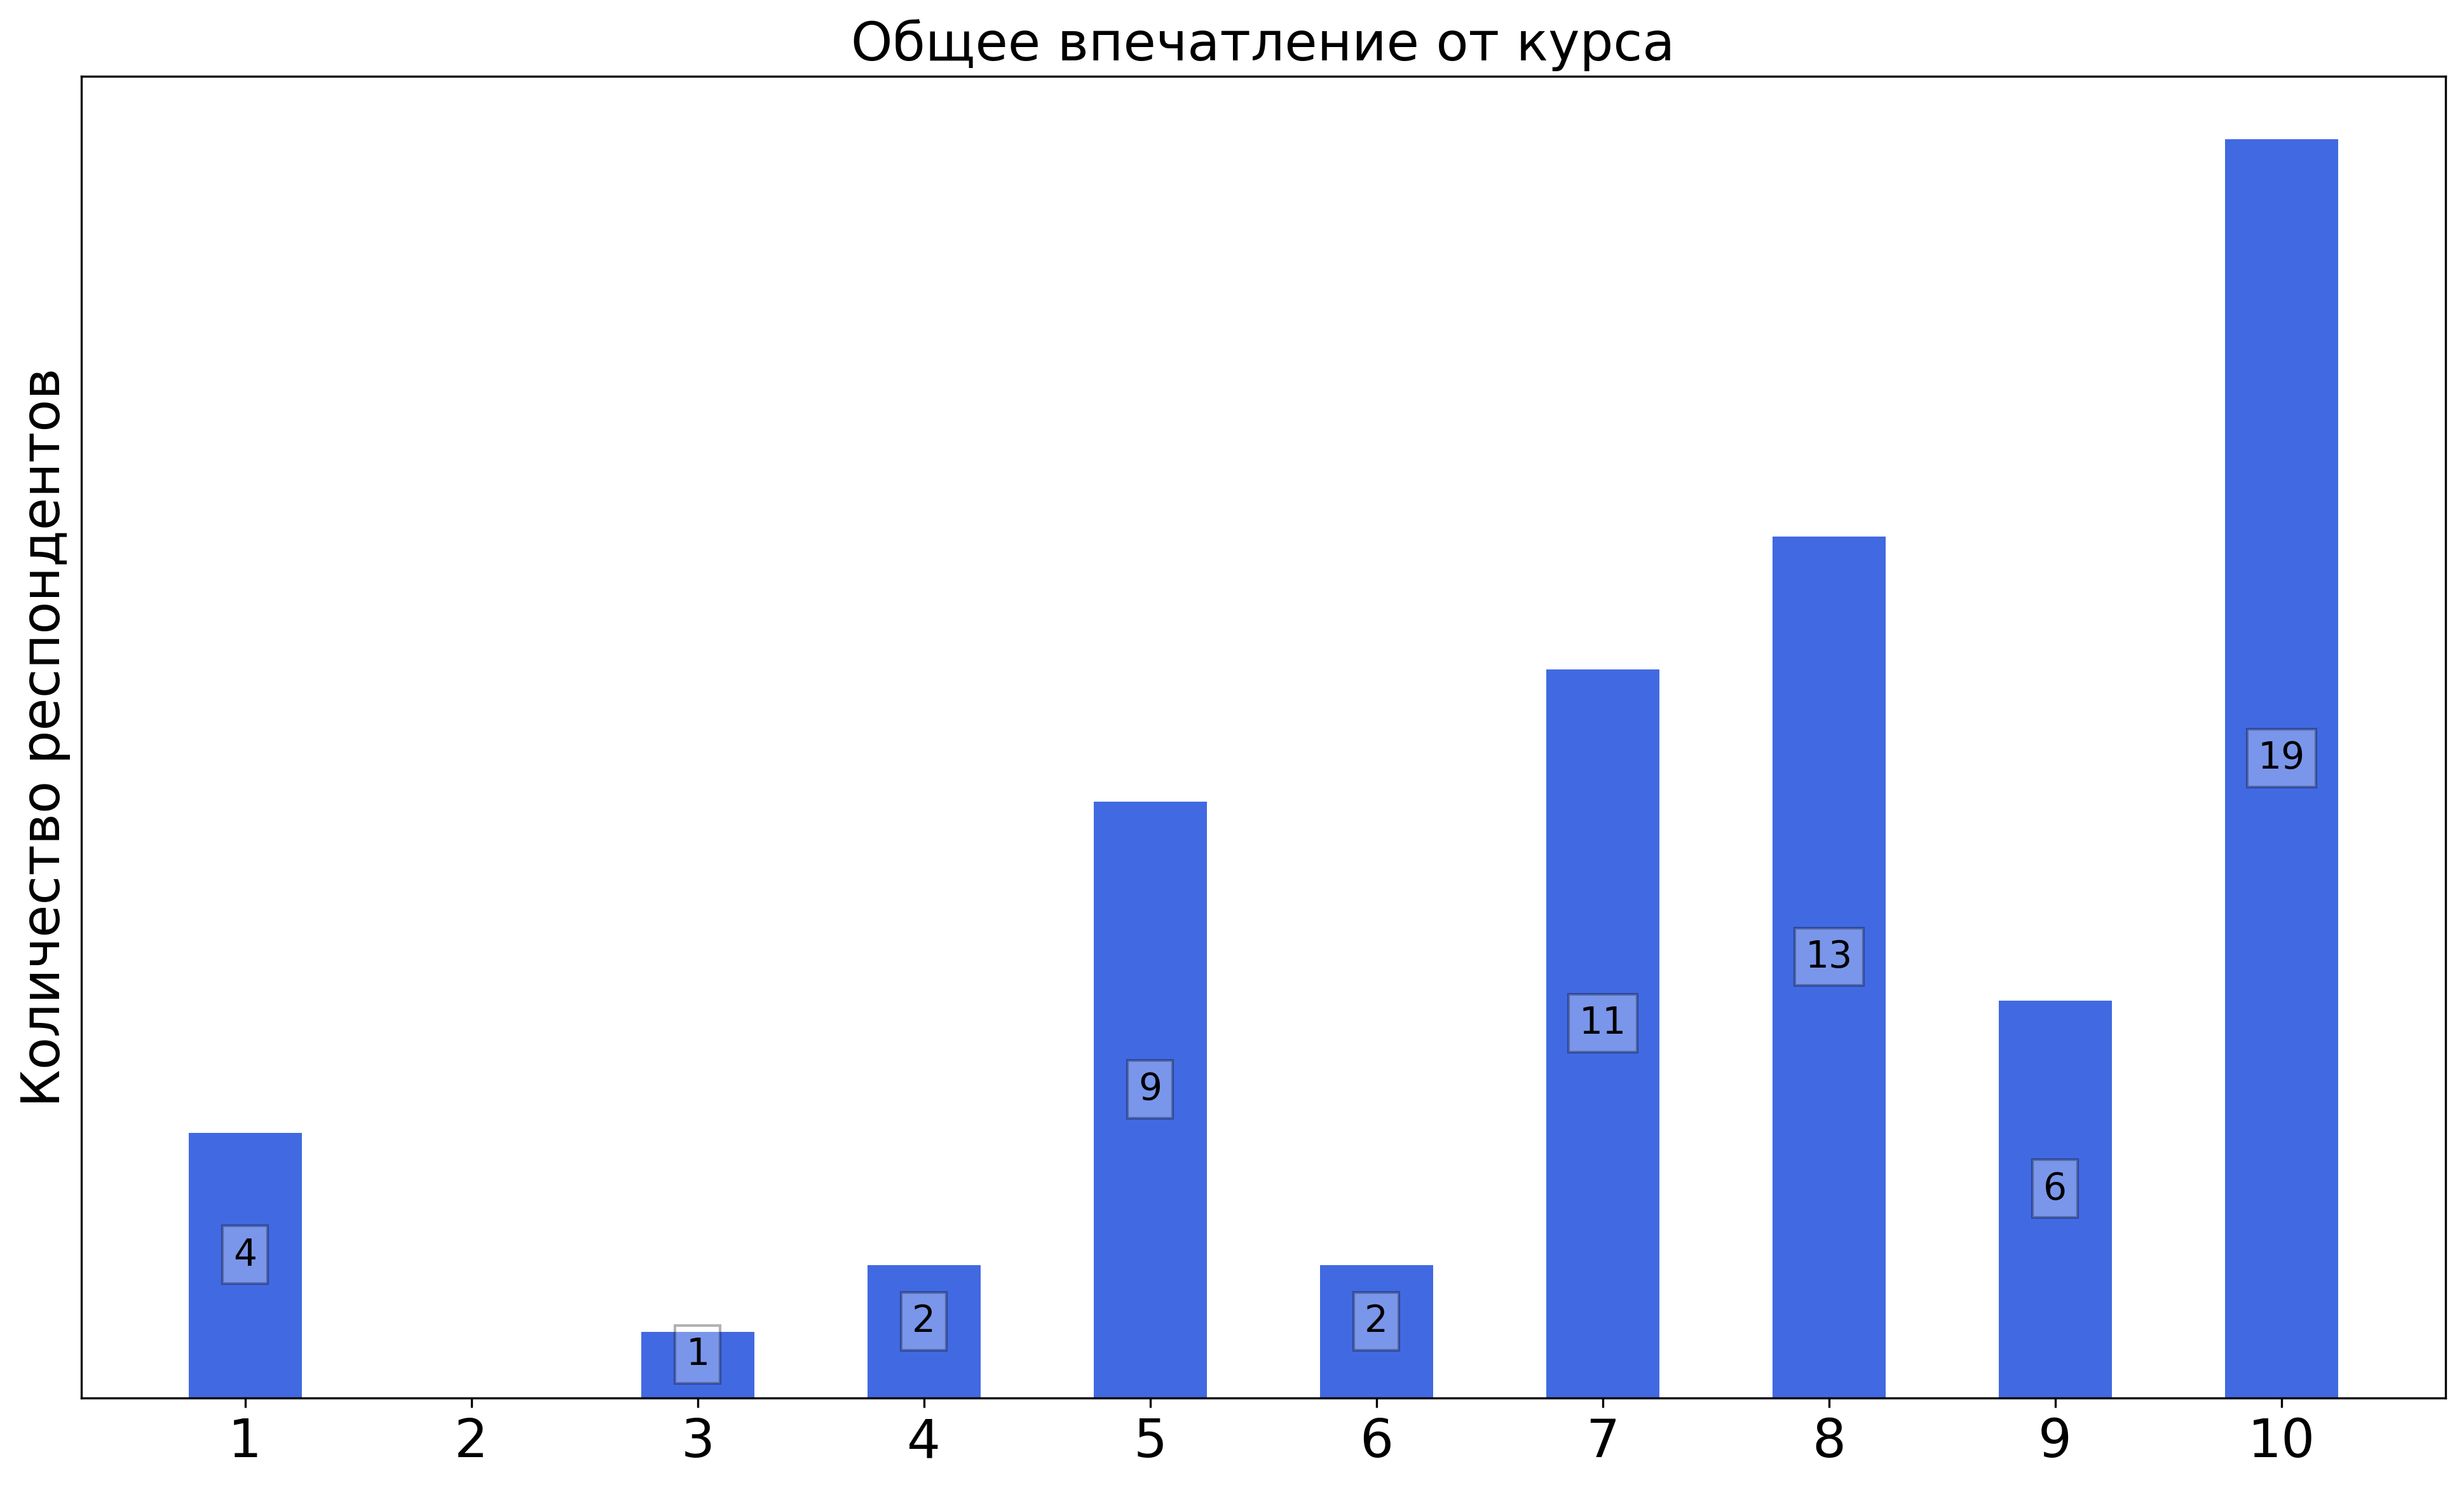
\includegraphics[width=\textwidth]{images/3 course/Радиофизическая лаборатория/general-0.png}
			\end{subfigure}
		\end{figure}

	\subsubsection{Материалы, использумые респондентами при изучении курса}

		\textit{В качестве источников информации студенты указали:} 
		\begin{itemize}
			\item методички к лабораторным работам.
		\end{itemize}


    \subsubsection{Отзыв студентов о лабораторных работах. Преподаватель: Антипов А.Е.}
		\begin{figure}[H]
			\centering
			\begin{subfigure}[b]{0.45\textwidth}
				\centering
				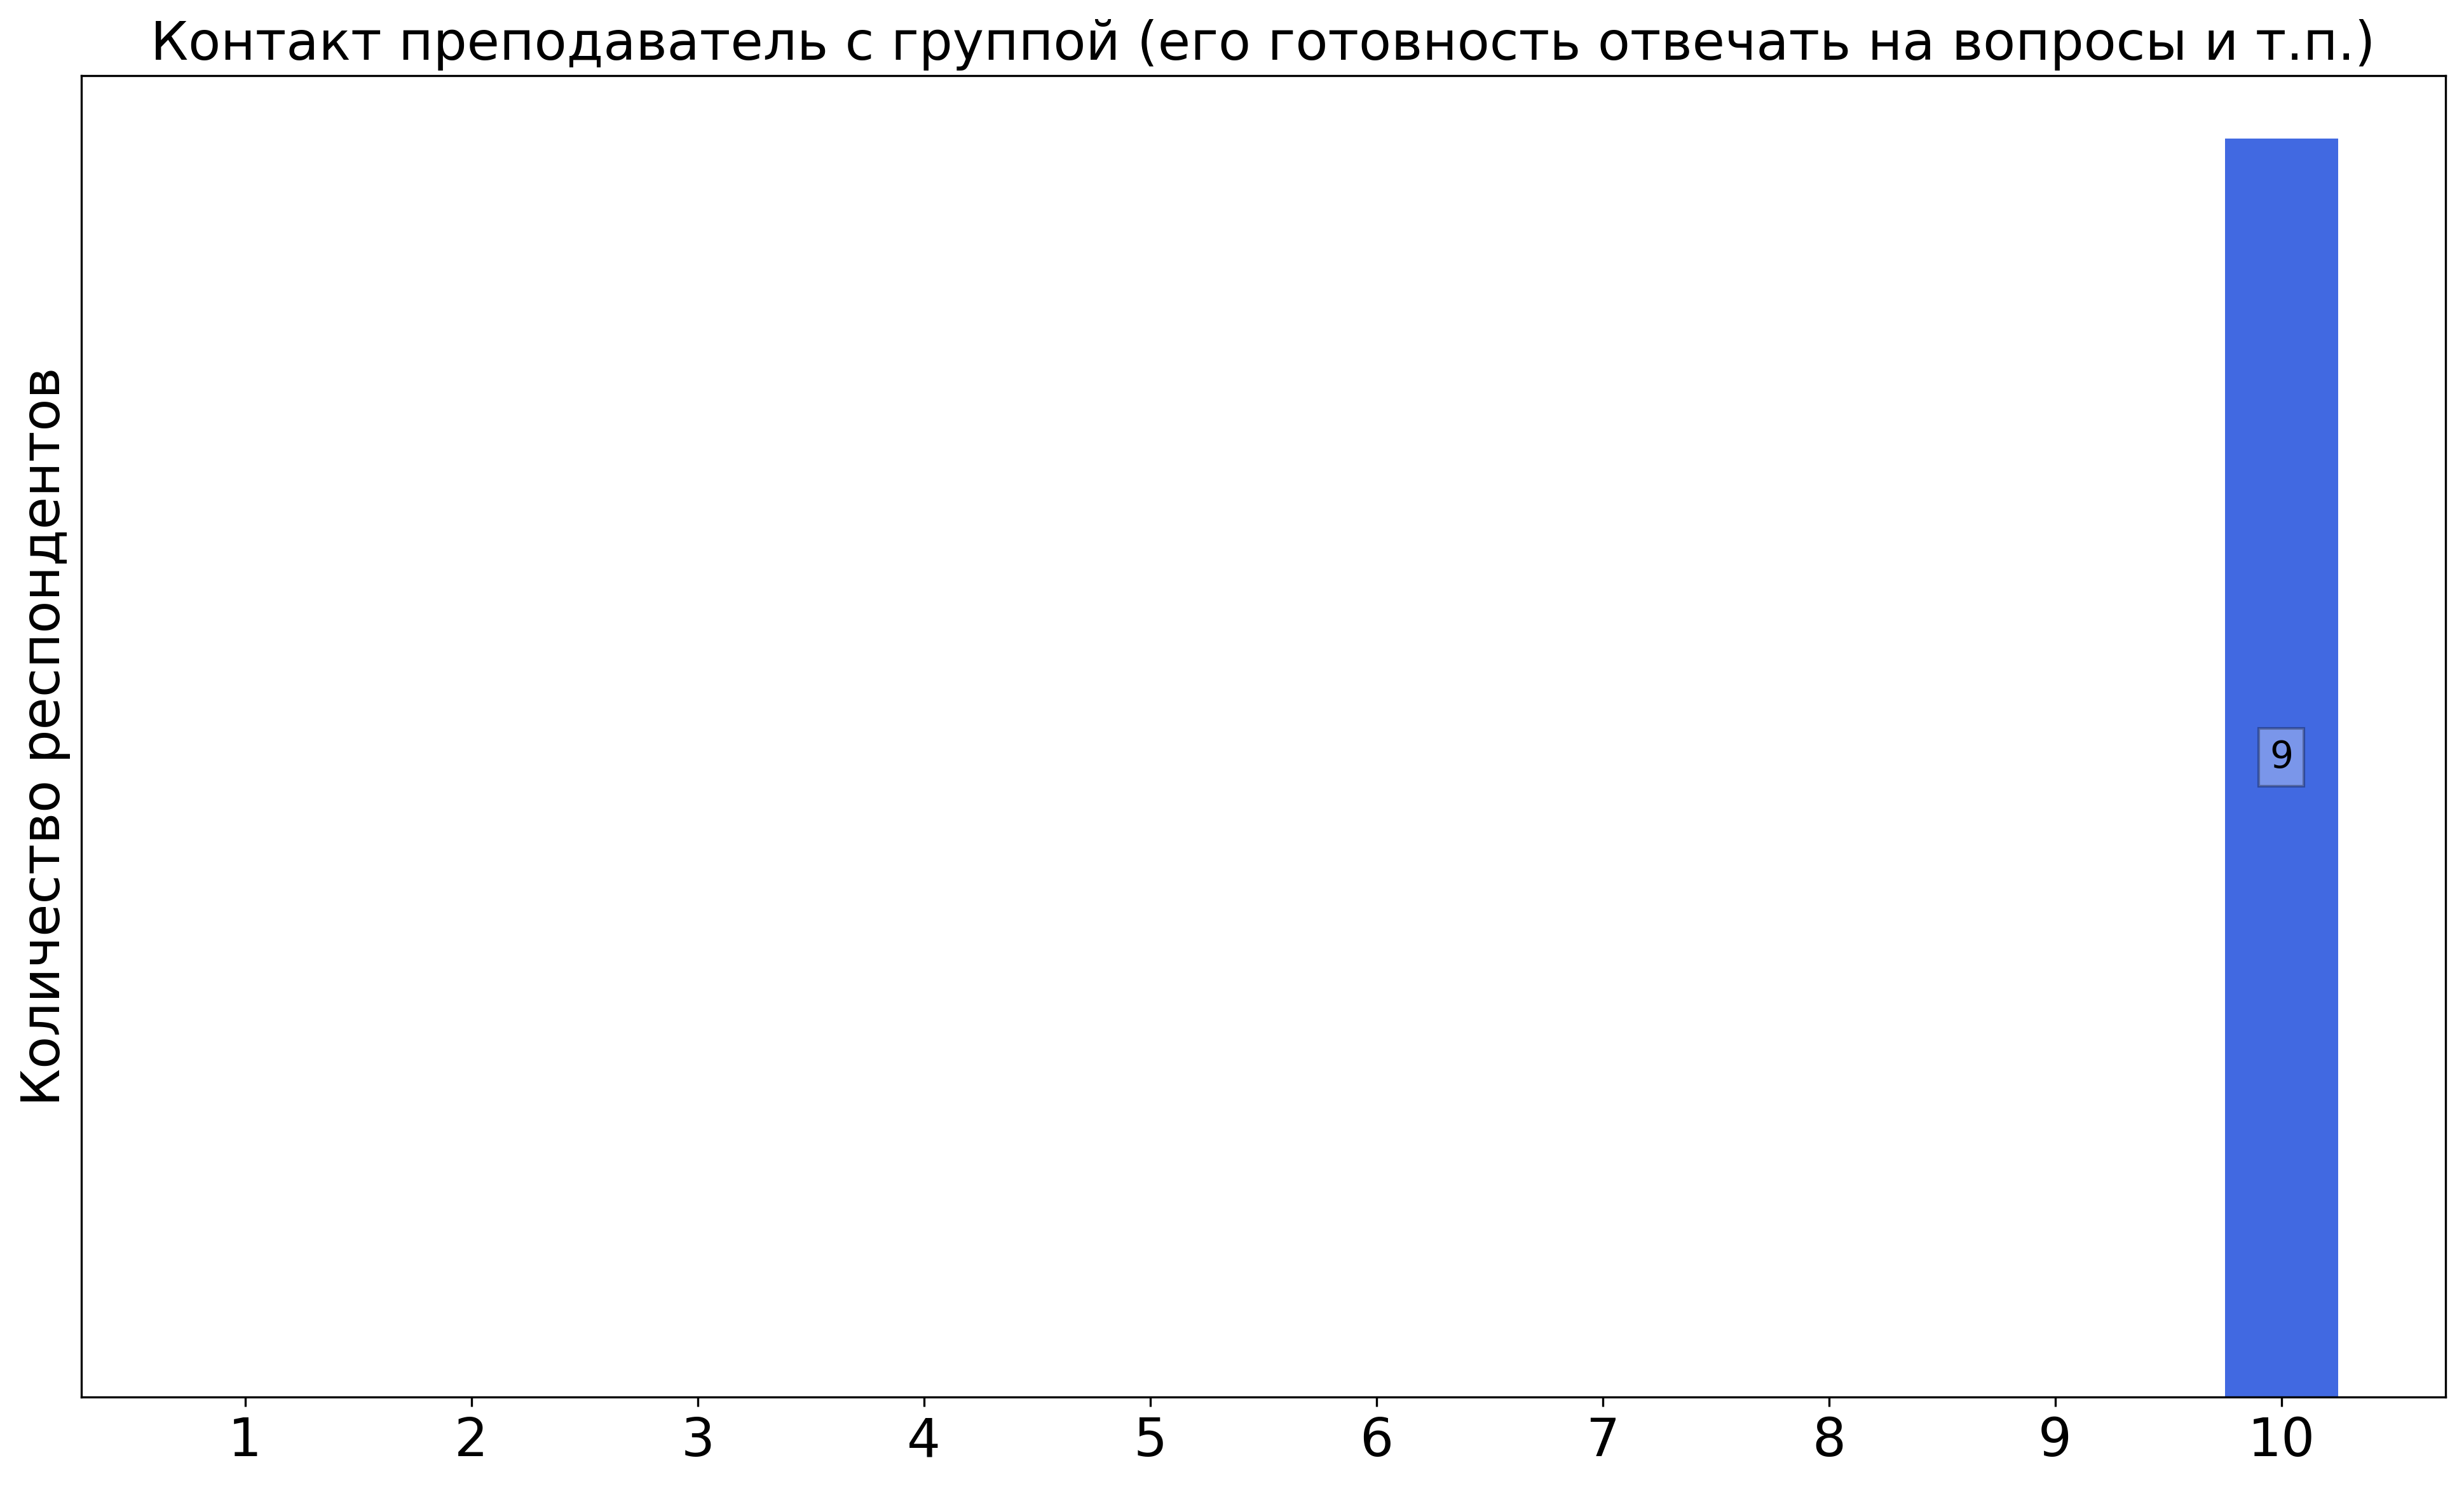
\includegraphics[width=\textwidth]{images/3 course/Радиофизическая лаборатория/labniks-marks-Борисов Д.А.-0.png}
			\end{subfigure}
			\begin{subfigure}[b]{0.45\textwidth}
				\centering
				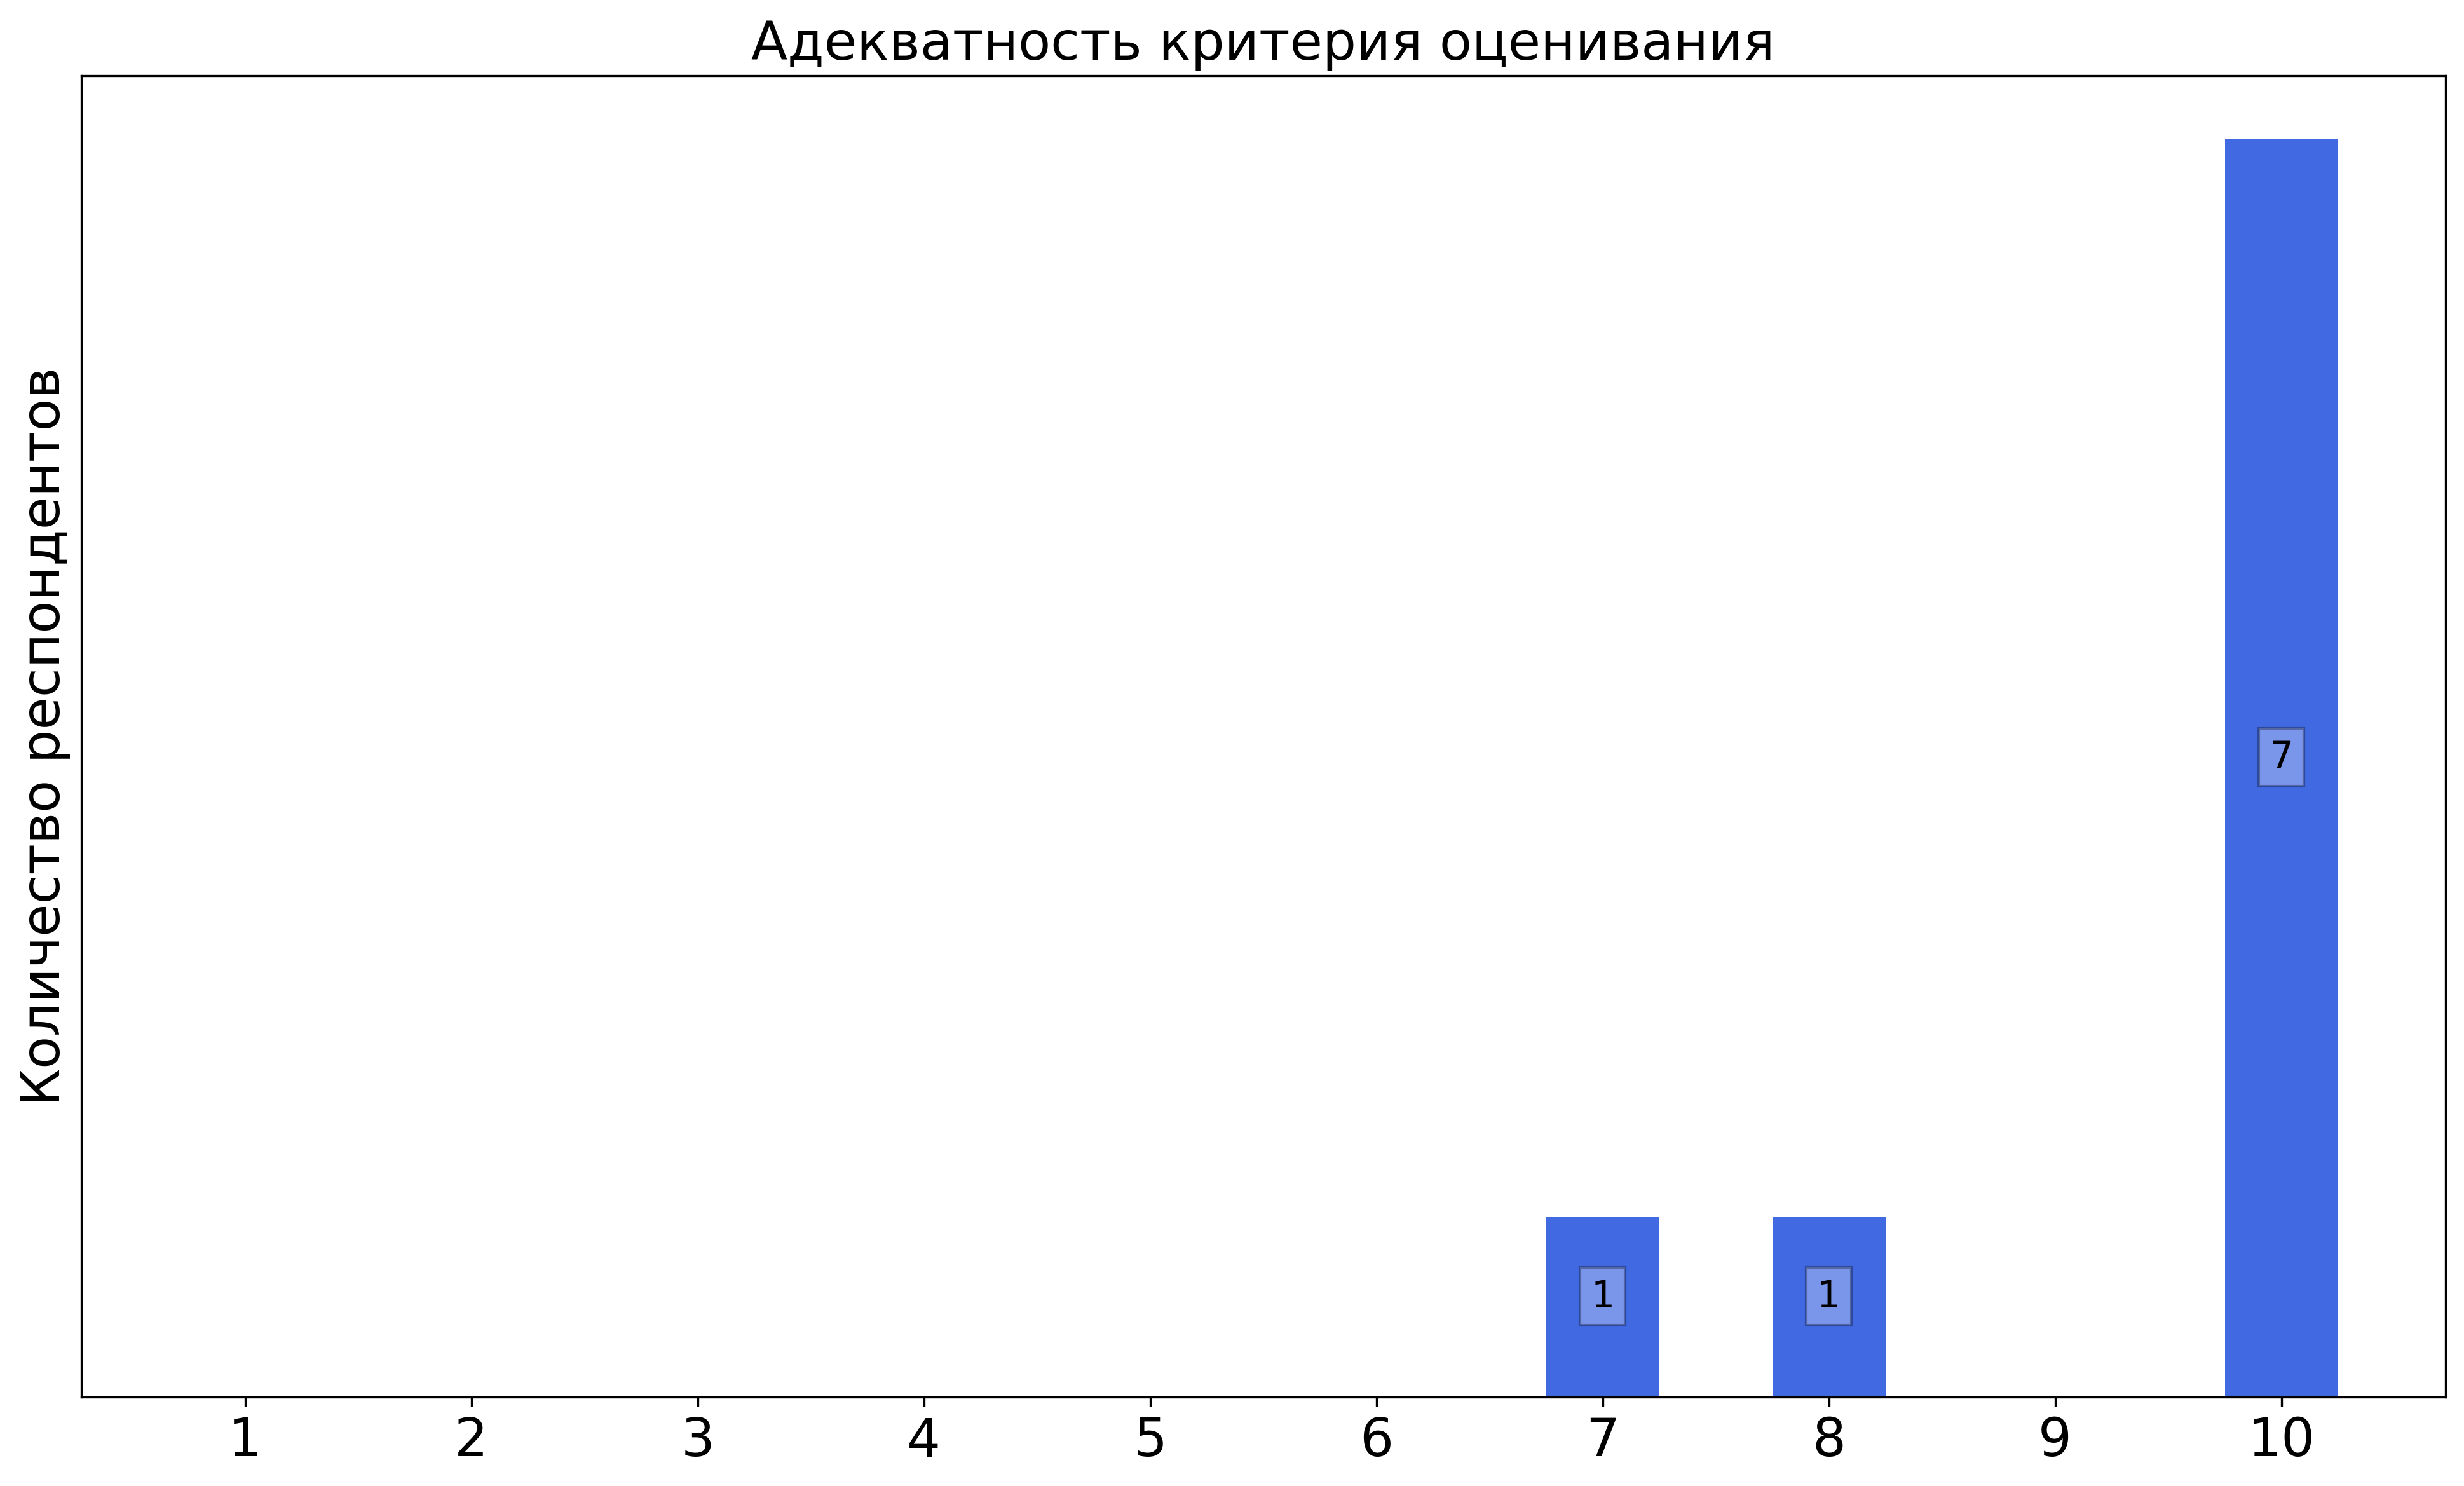
\includegraphics[width=\textwidth]{images/3 course/Радиофизическая лаборатория/labniks-marks-Борисов Д.А.-1.png}
			\end{subfigure}
			\begin{subfigure}[b]{0.45\textwidth}
				\centering
				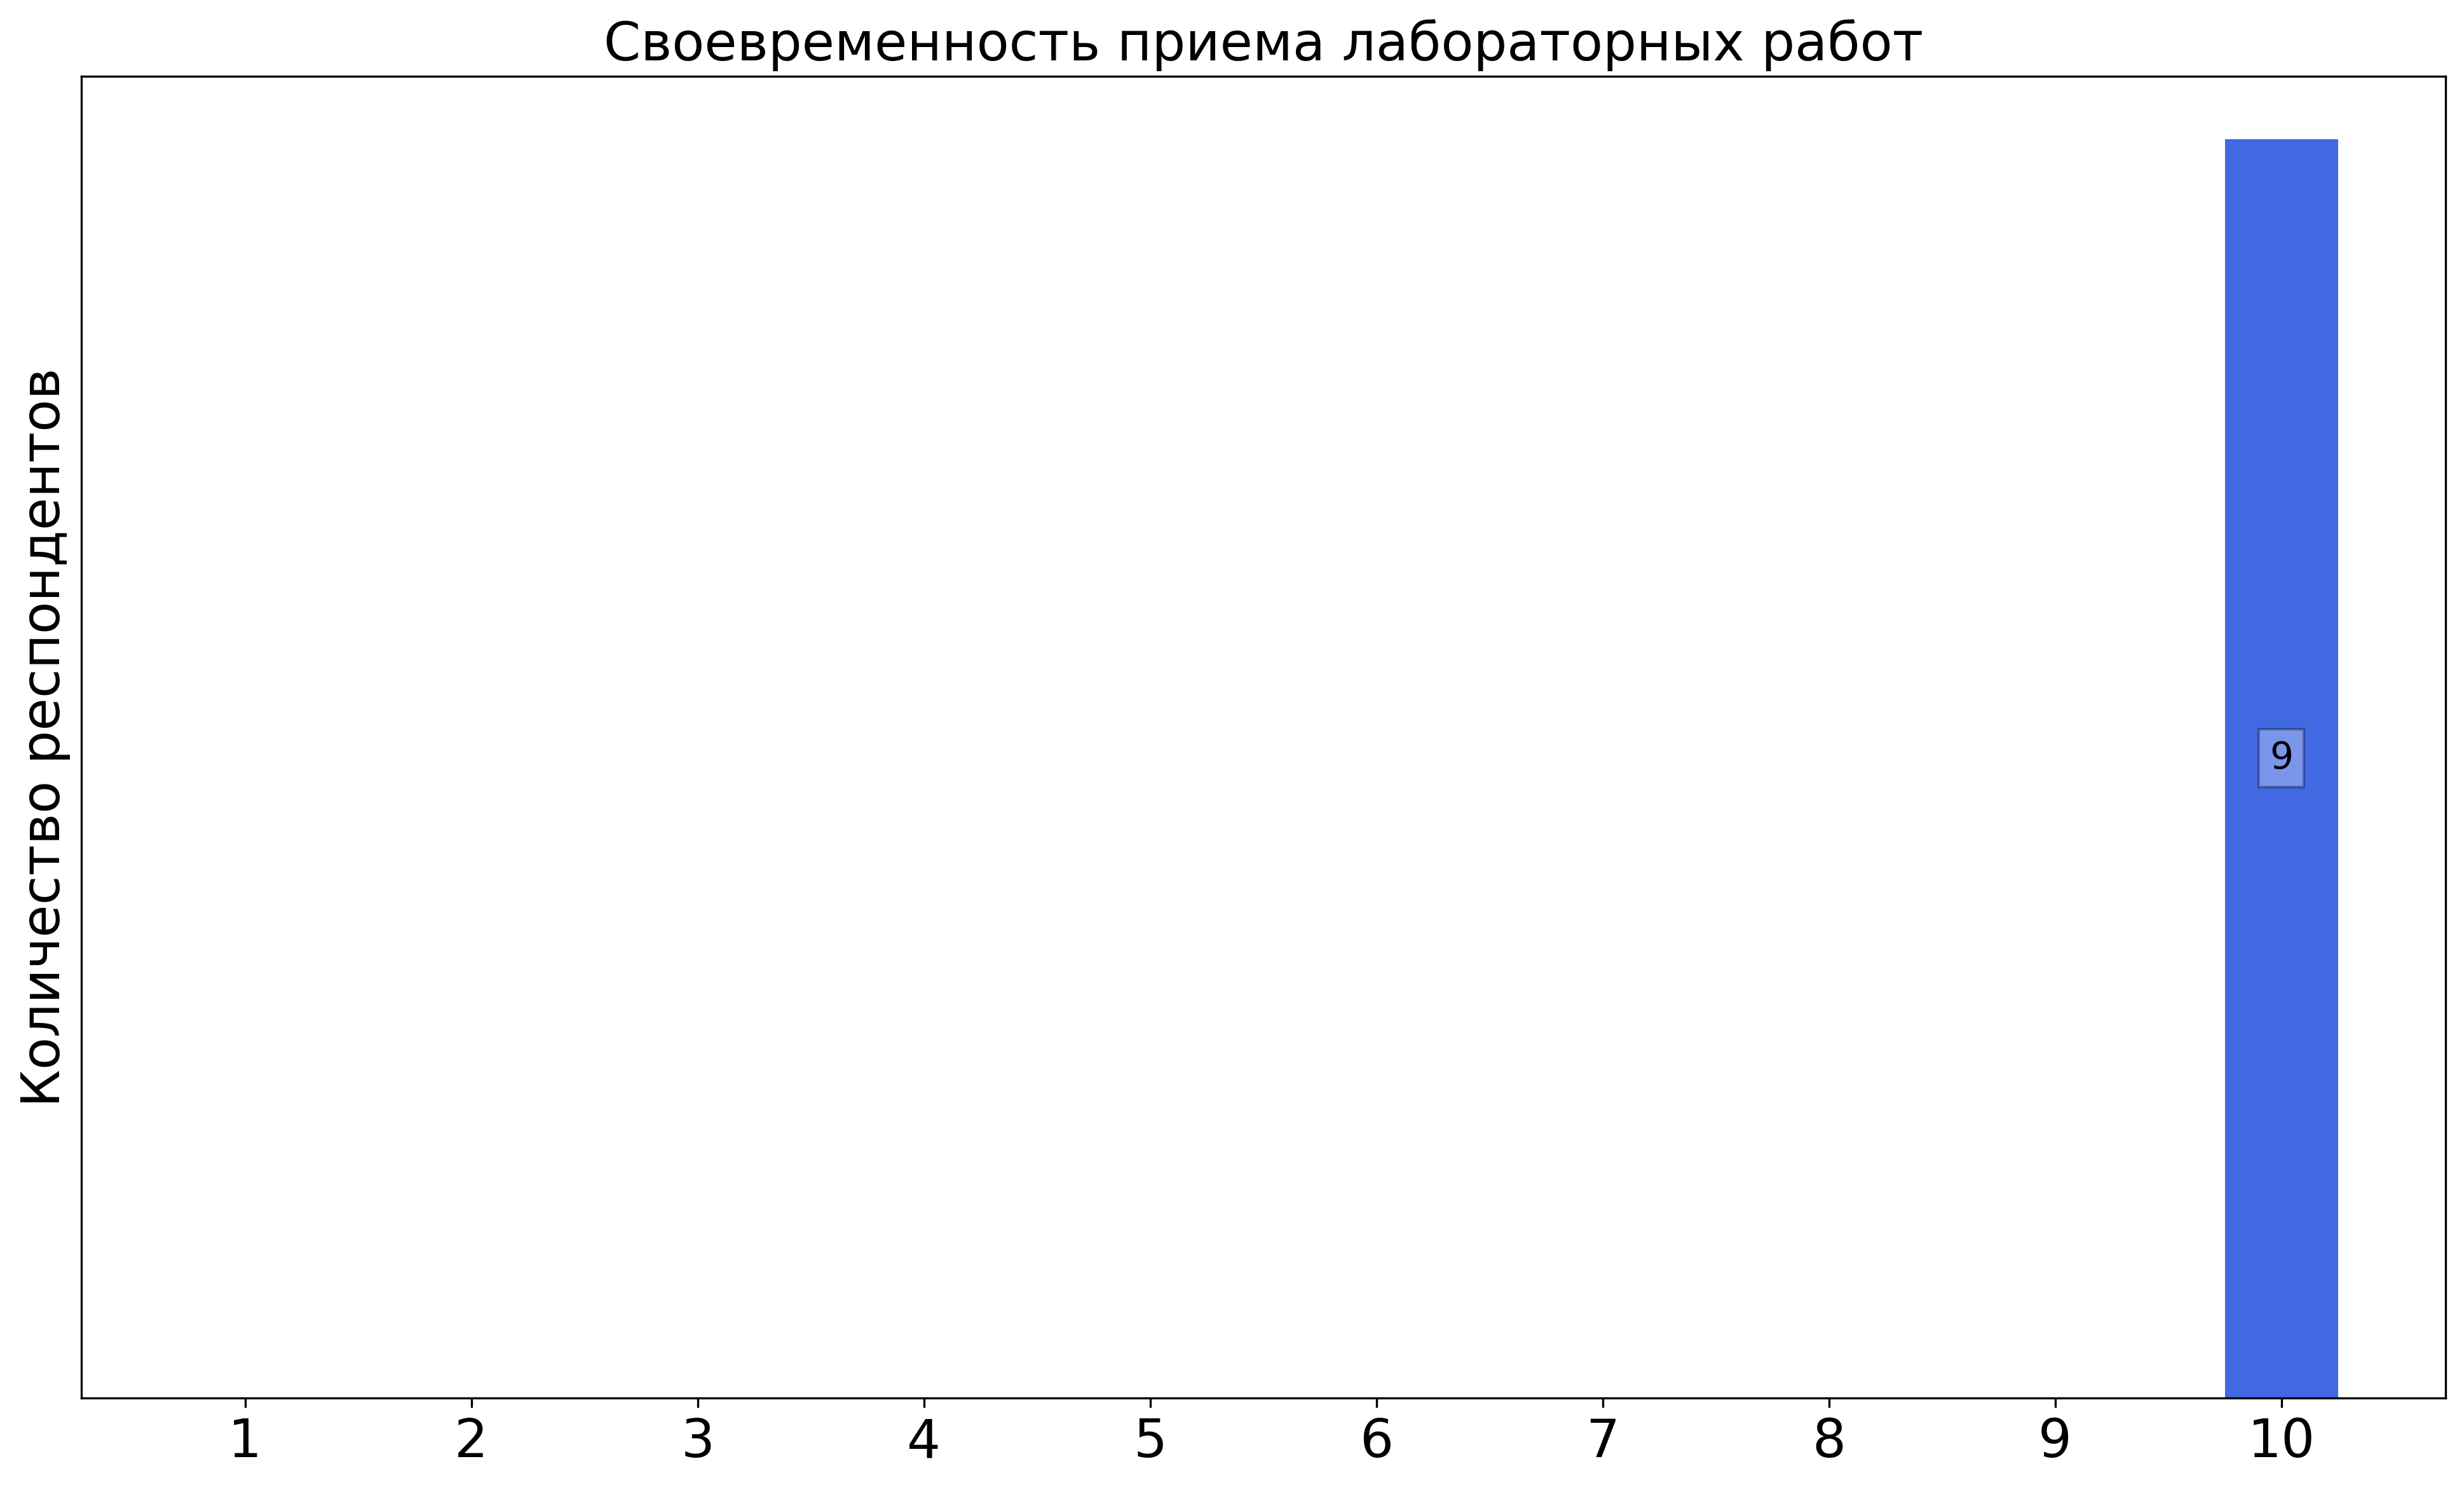
\includegraphics[width=\textwidth]{images/3 course/Радиофизическая лаборатория/labniks-marks-Борисов Д.А.-2.png}
			\end{subfigure}
			\begin{subfigure}[b]{0.45\textwidth}
				\centering
				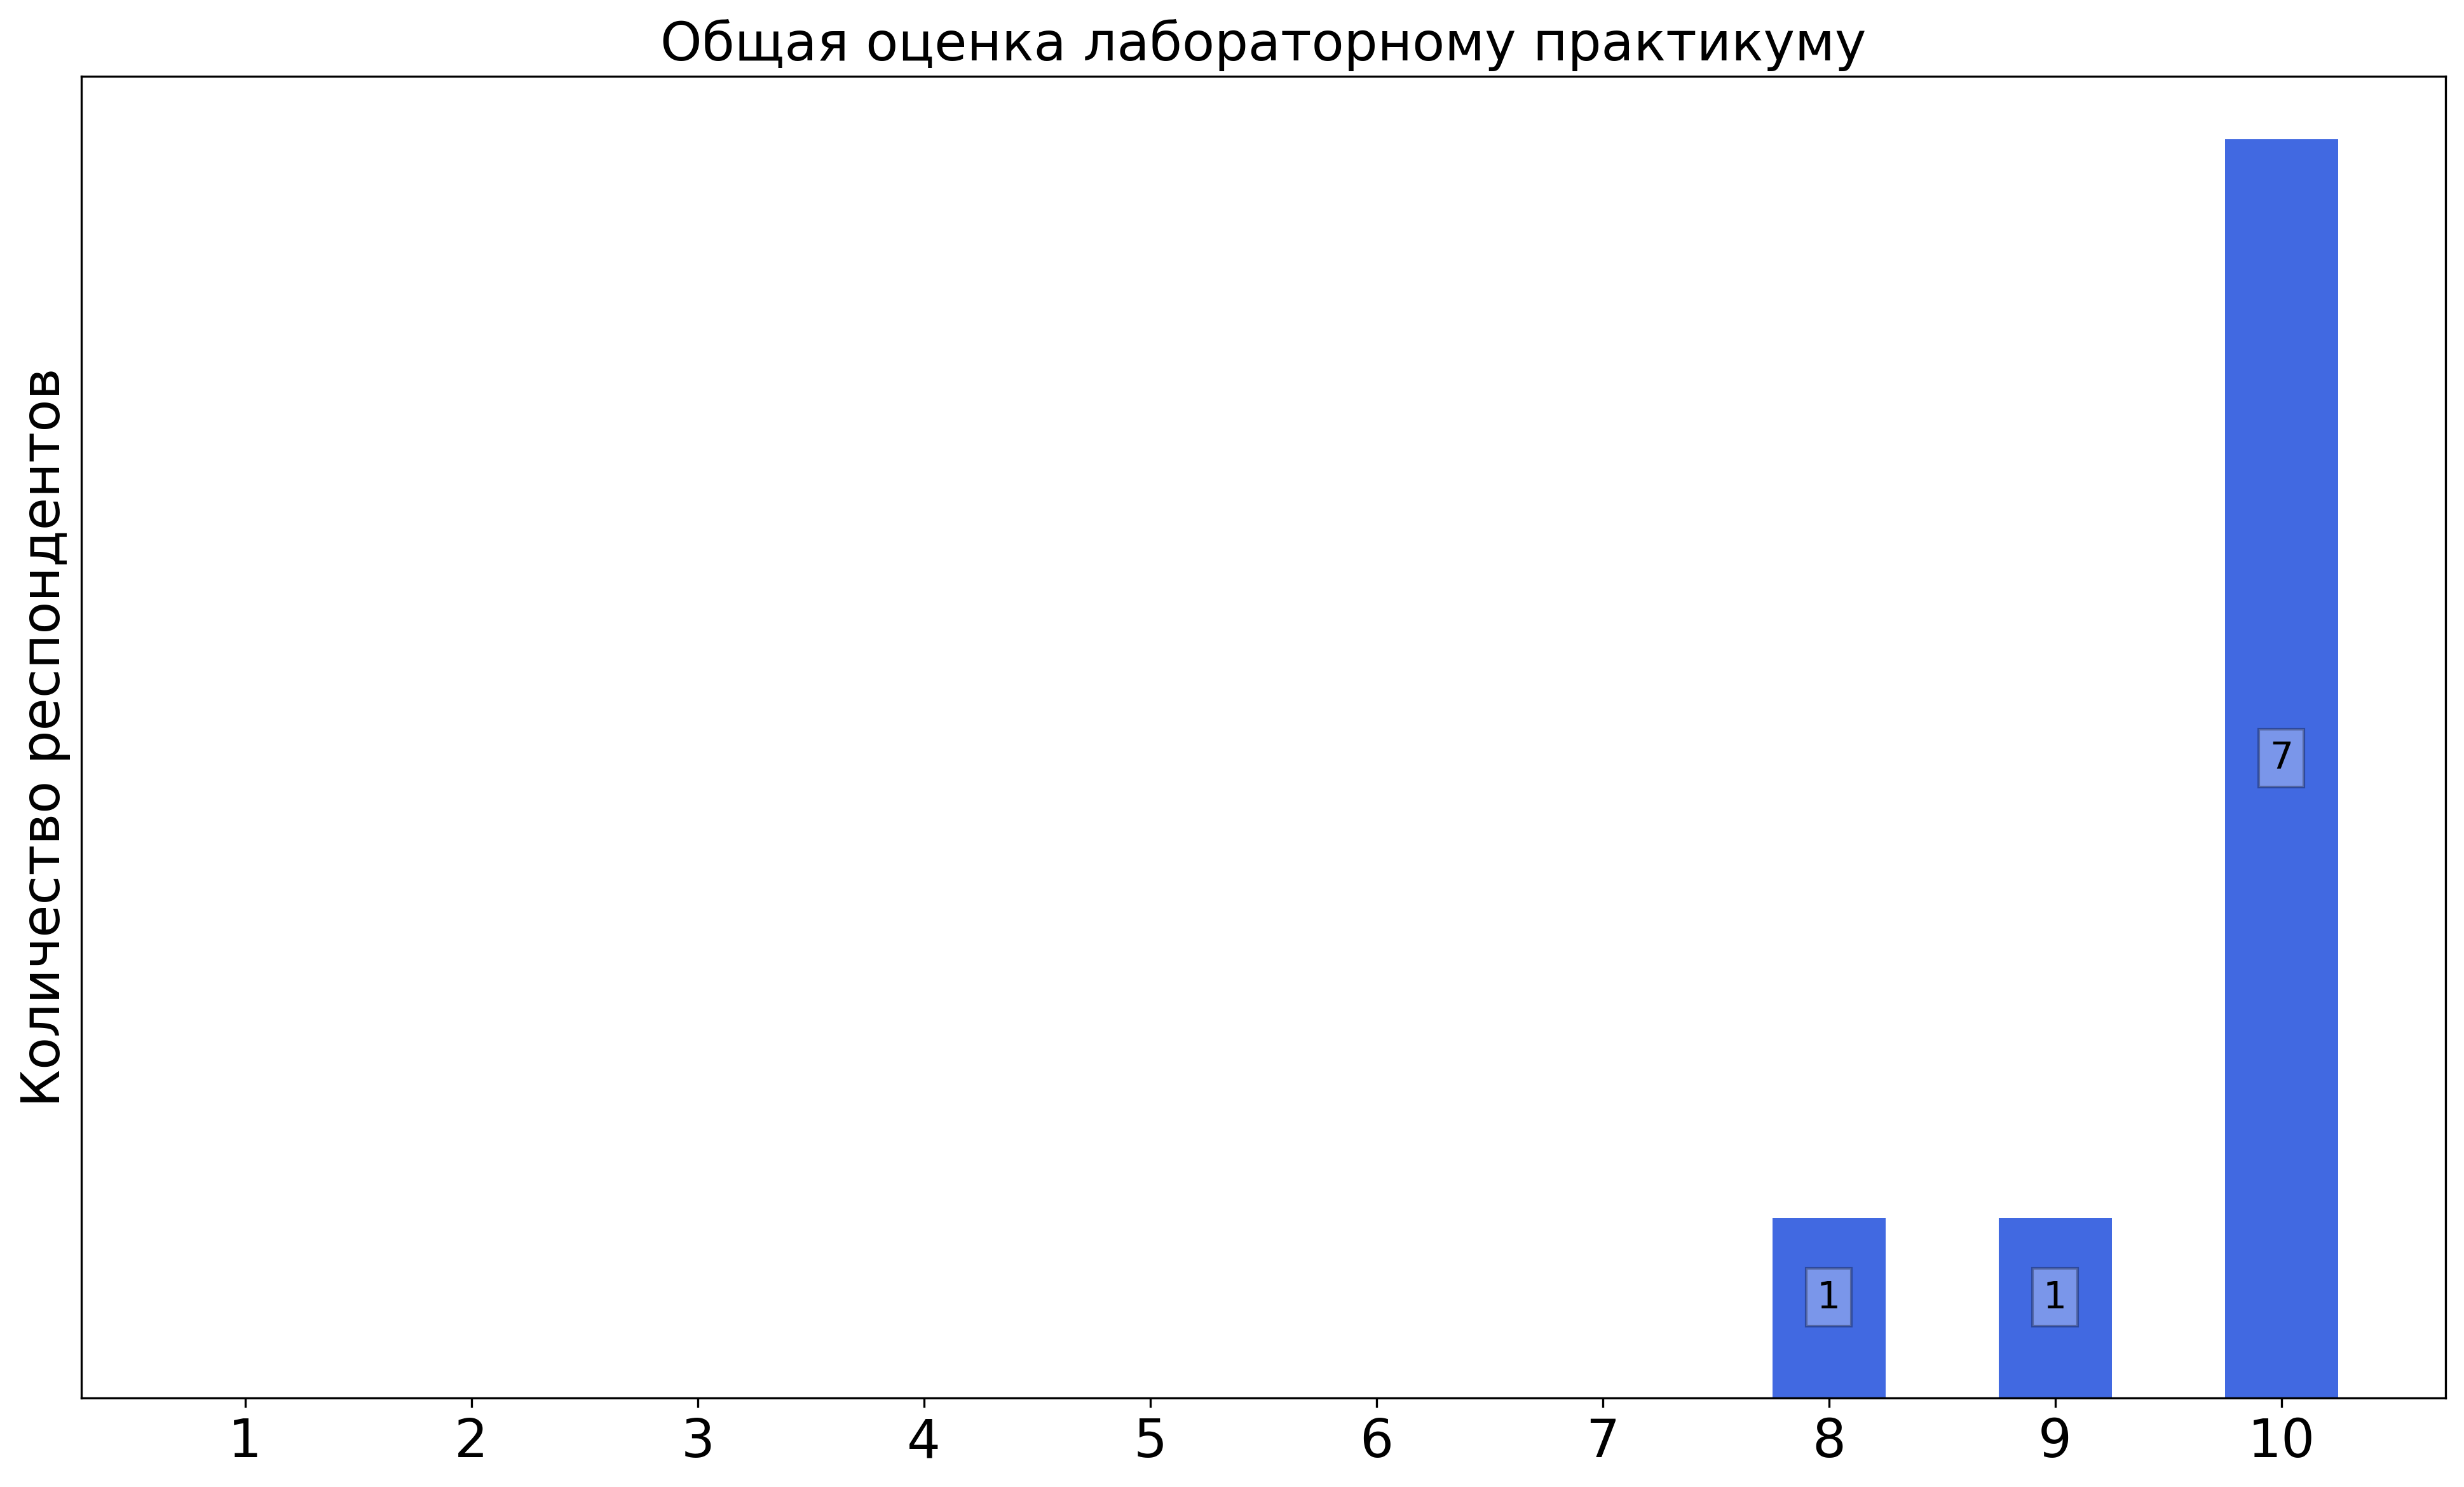
\includegraphics[width=\textwidth]{images/3 course/Радиофизическая лаборатория/labniks-marks-Борисов Д.А.-3.png}
			\end{subfigure}	
			\caption{Оценки респондентов о качестве преподавания лабораторных работ}
		\end{figure}

		\textbf{Комментарии студентов о преподавателе\protect\footnote{сохранены оригинальные орфография и пунктуация}}
            \begin{commentbox} 
                Предмет в целом халявный, но если ботать - неприятно. Лично у меня эта теория усваивается плохо 
            \end{commentbox} 


    \subsubsection{Отзыв студентов о лабораторных работах. Преподаватель: Борисов Д.А.}
        \begin{figure}[H]
            \centering
            \begin{subfigure}[b]{0.45\textwidth}
                \centering
                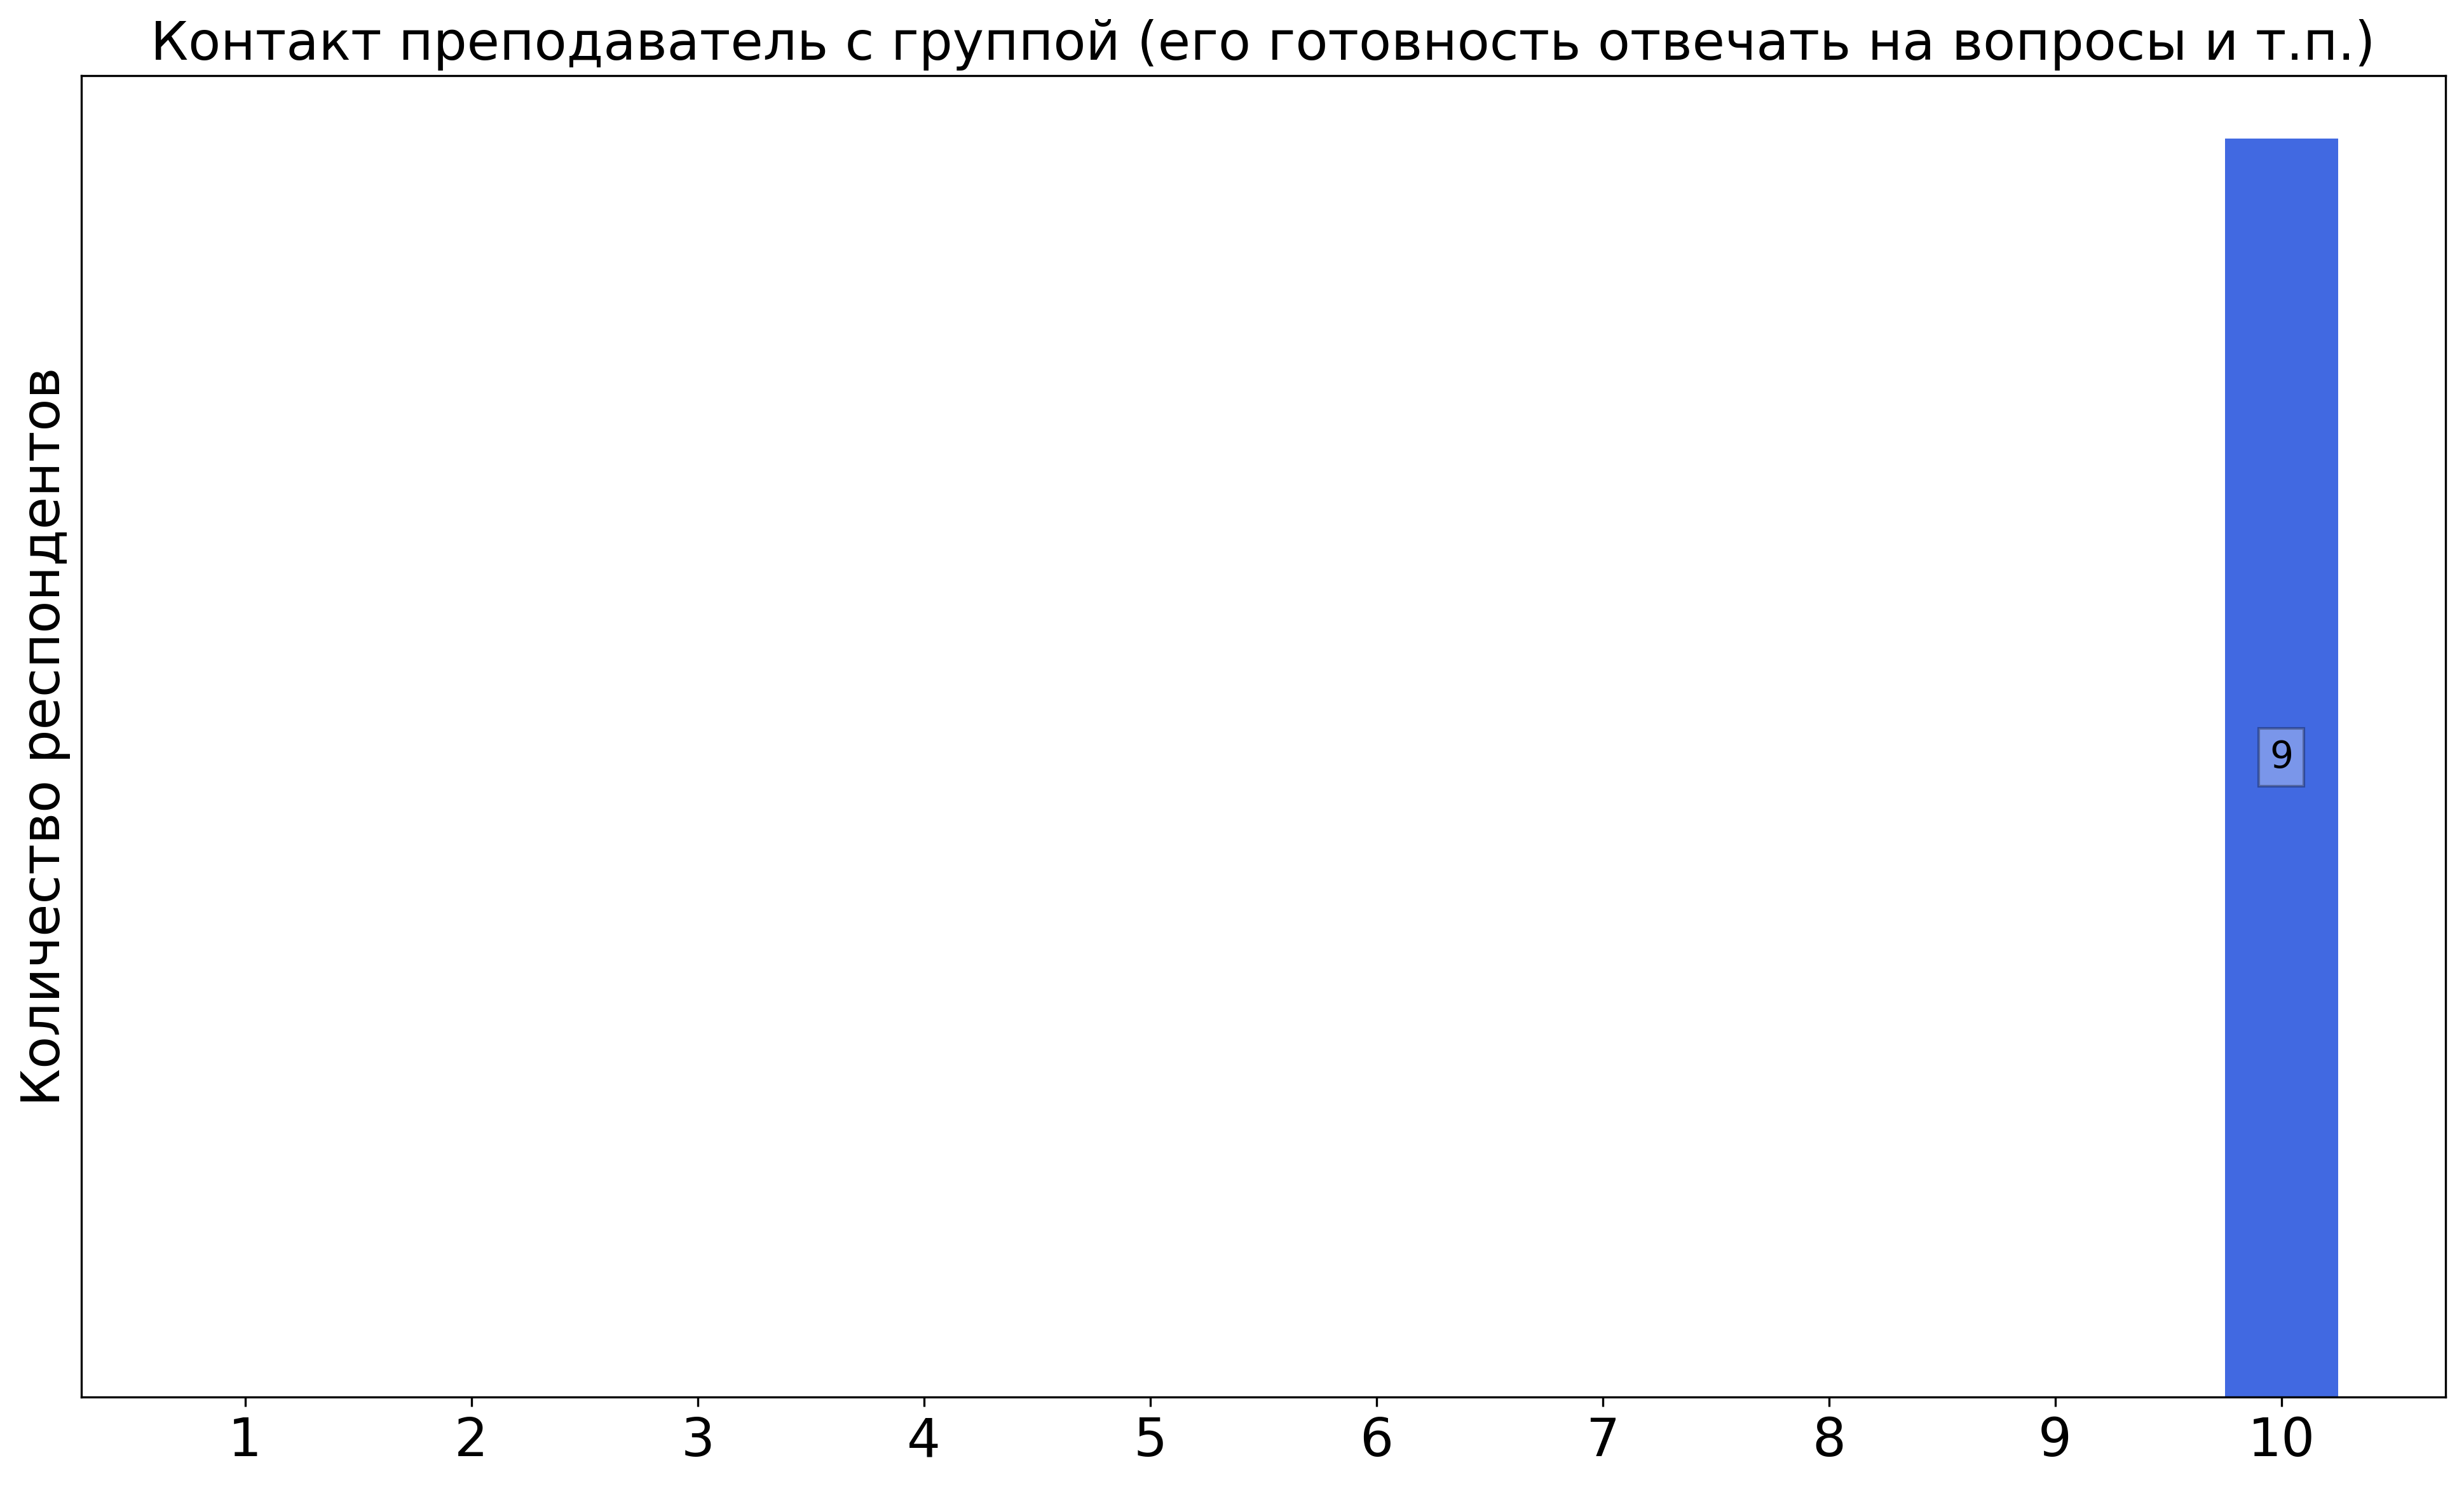
\includegraphics[width=\textwidth]{images/3 course/Радиофизическая лаборатория/labniks-marks-Борисов Д.А.-0.png}
            \end{subfigure}
            \begin{subfigure}[b]{0.45\textwidth}
                \centering
                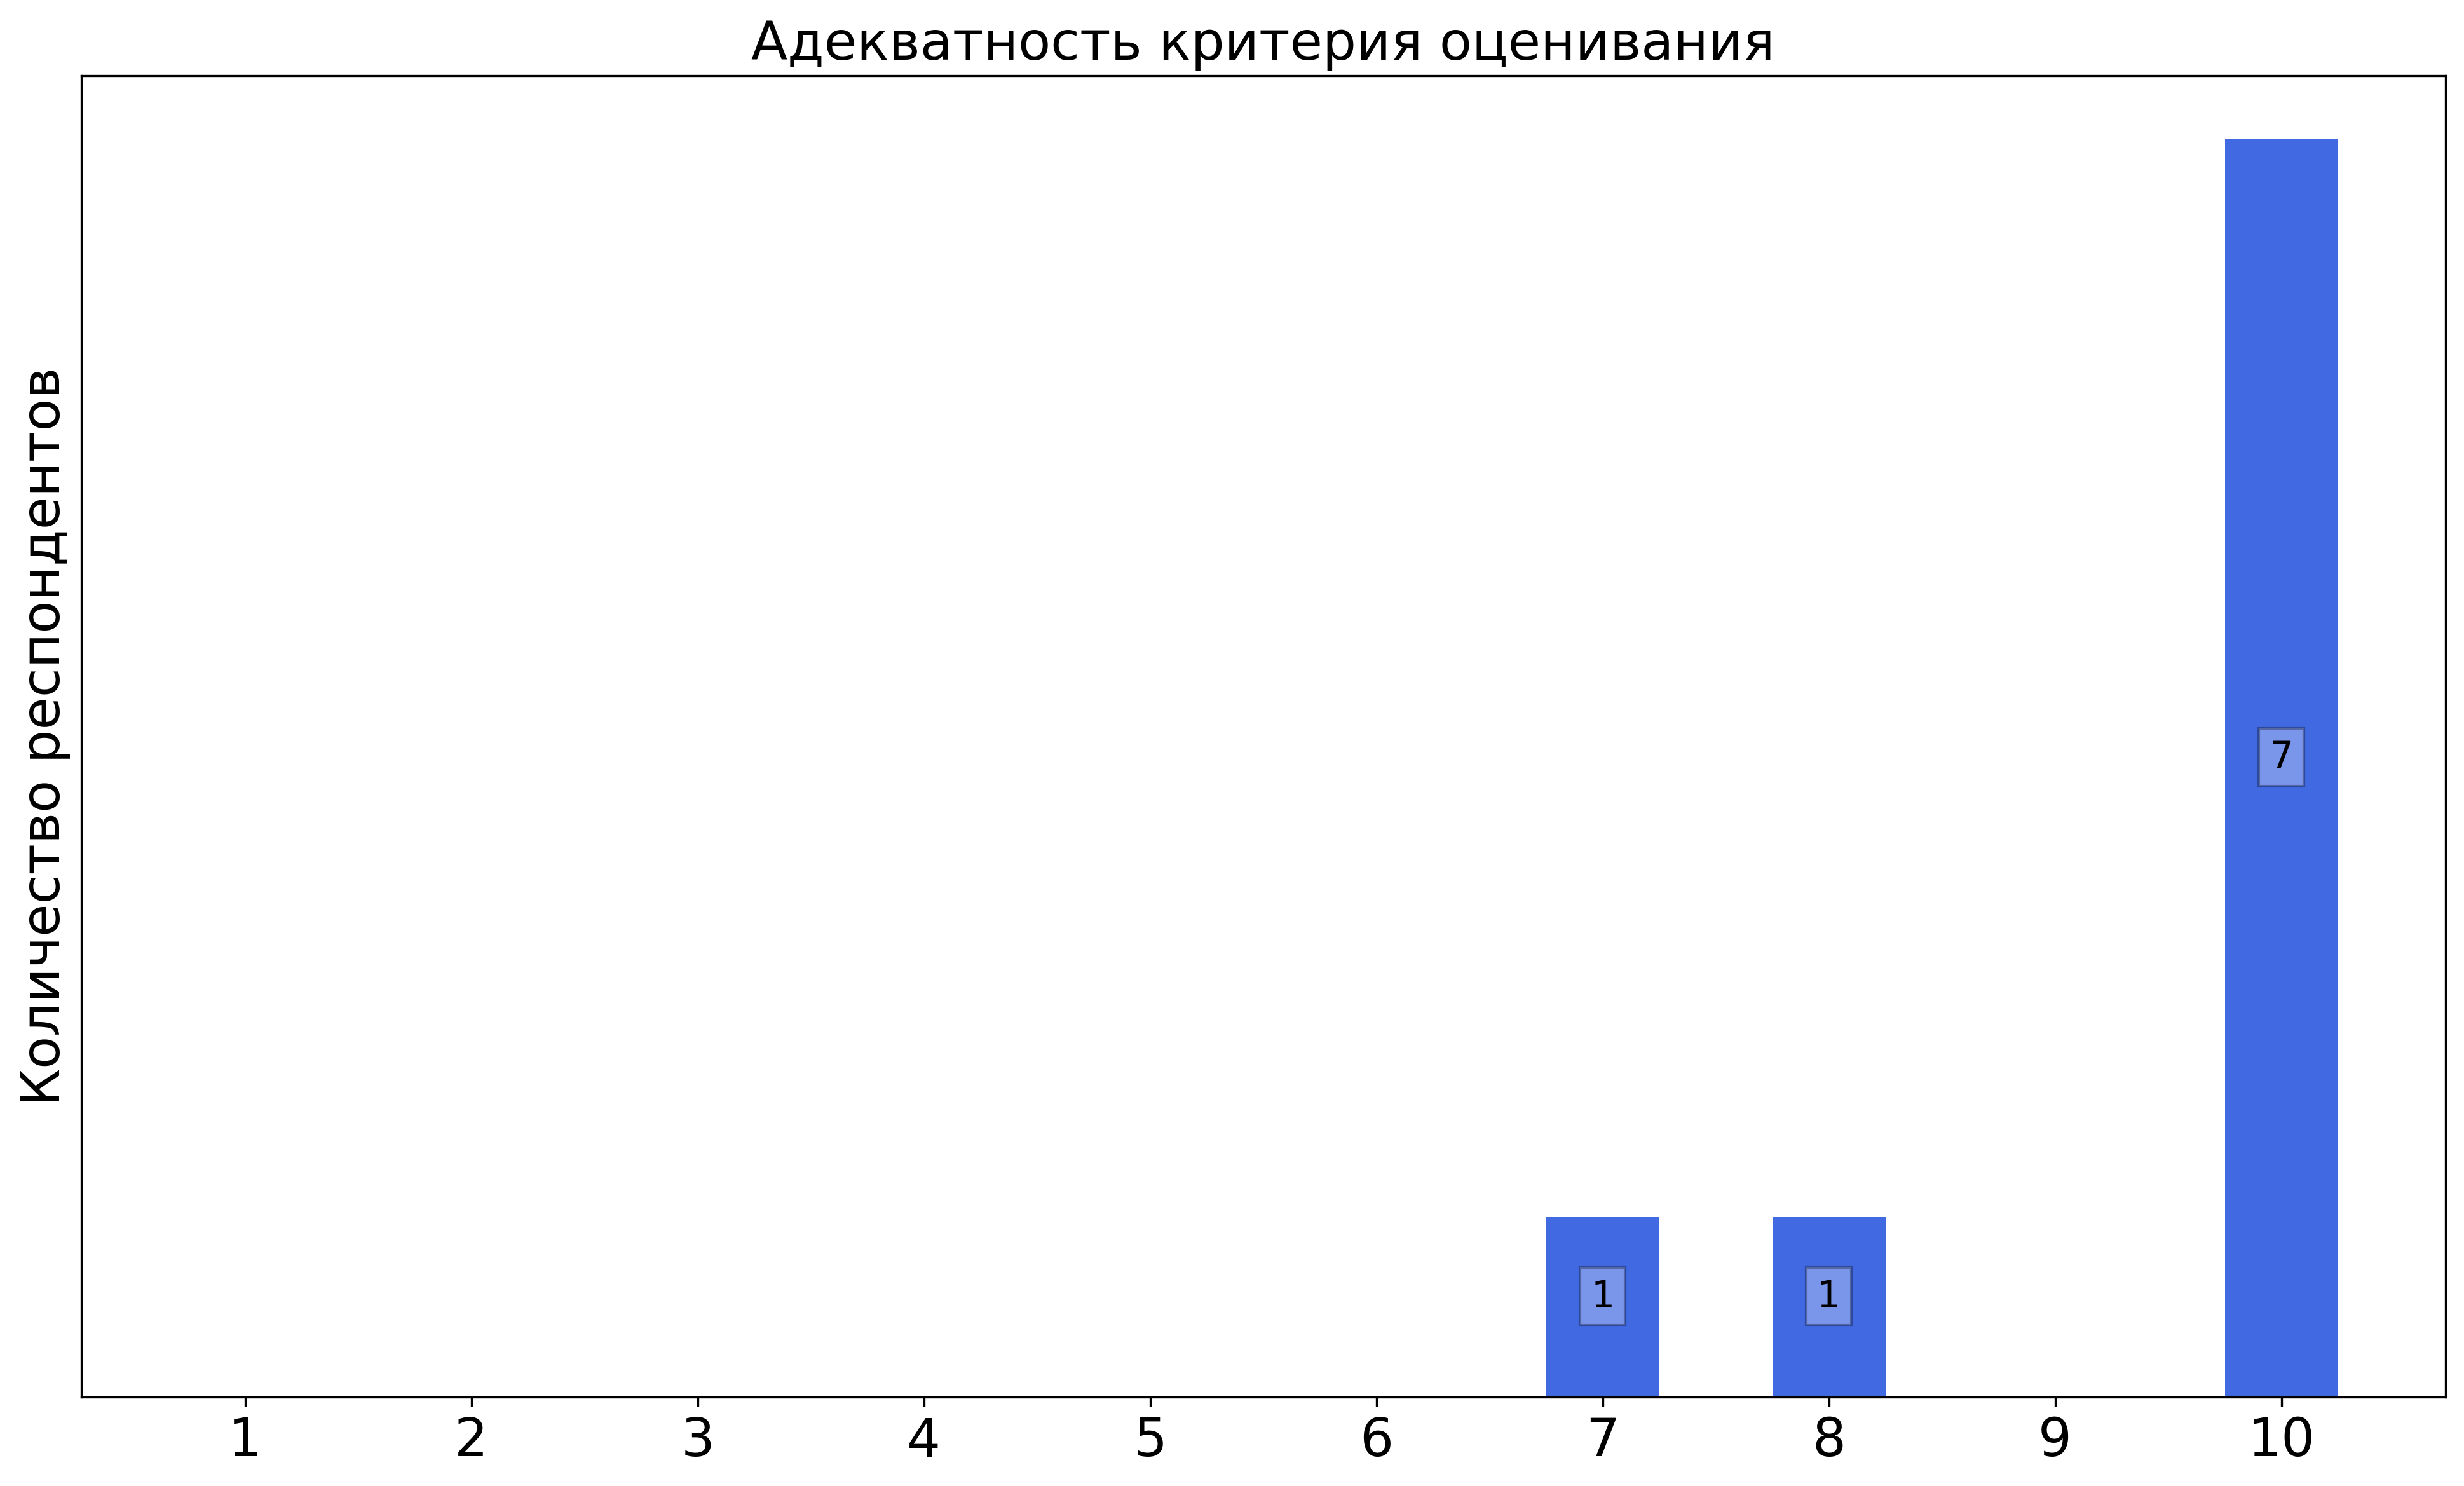
\includegraphics[width=\textwidth]{images/3 course/Радиофизическая лаборатория/labniks-marks-Борисов Д.А.-1.png}
            \end{subfigure}
            \begin{subfigure}[b]{0.45\textwidth}
                \centering
                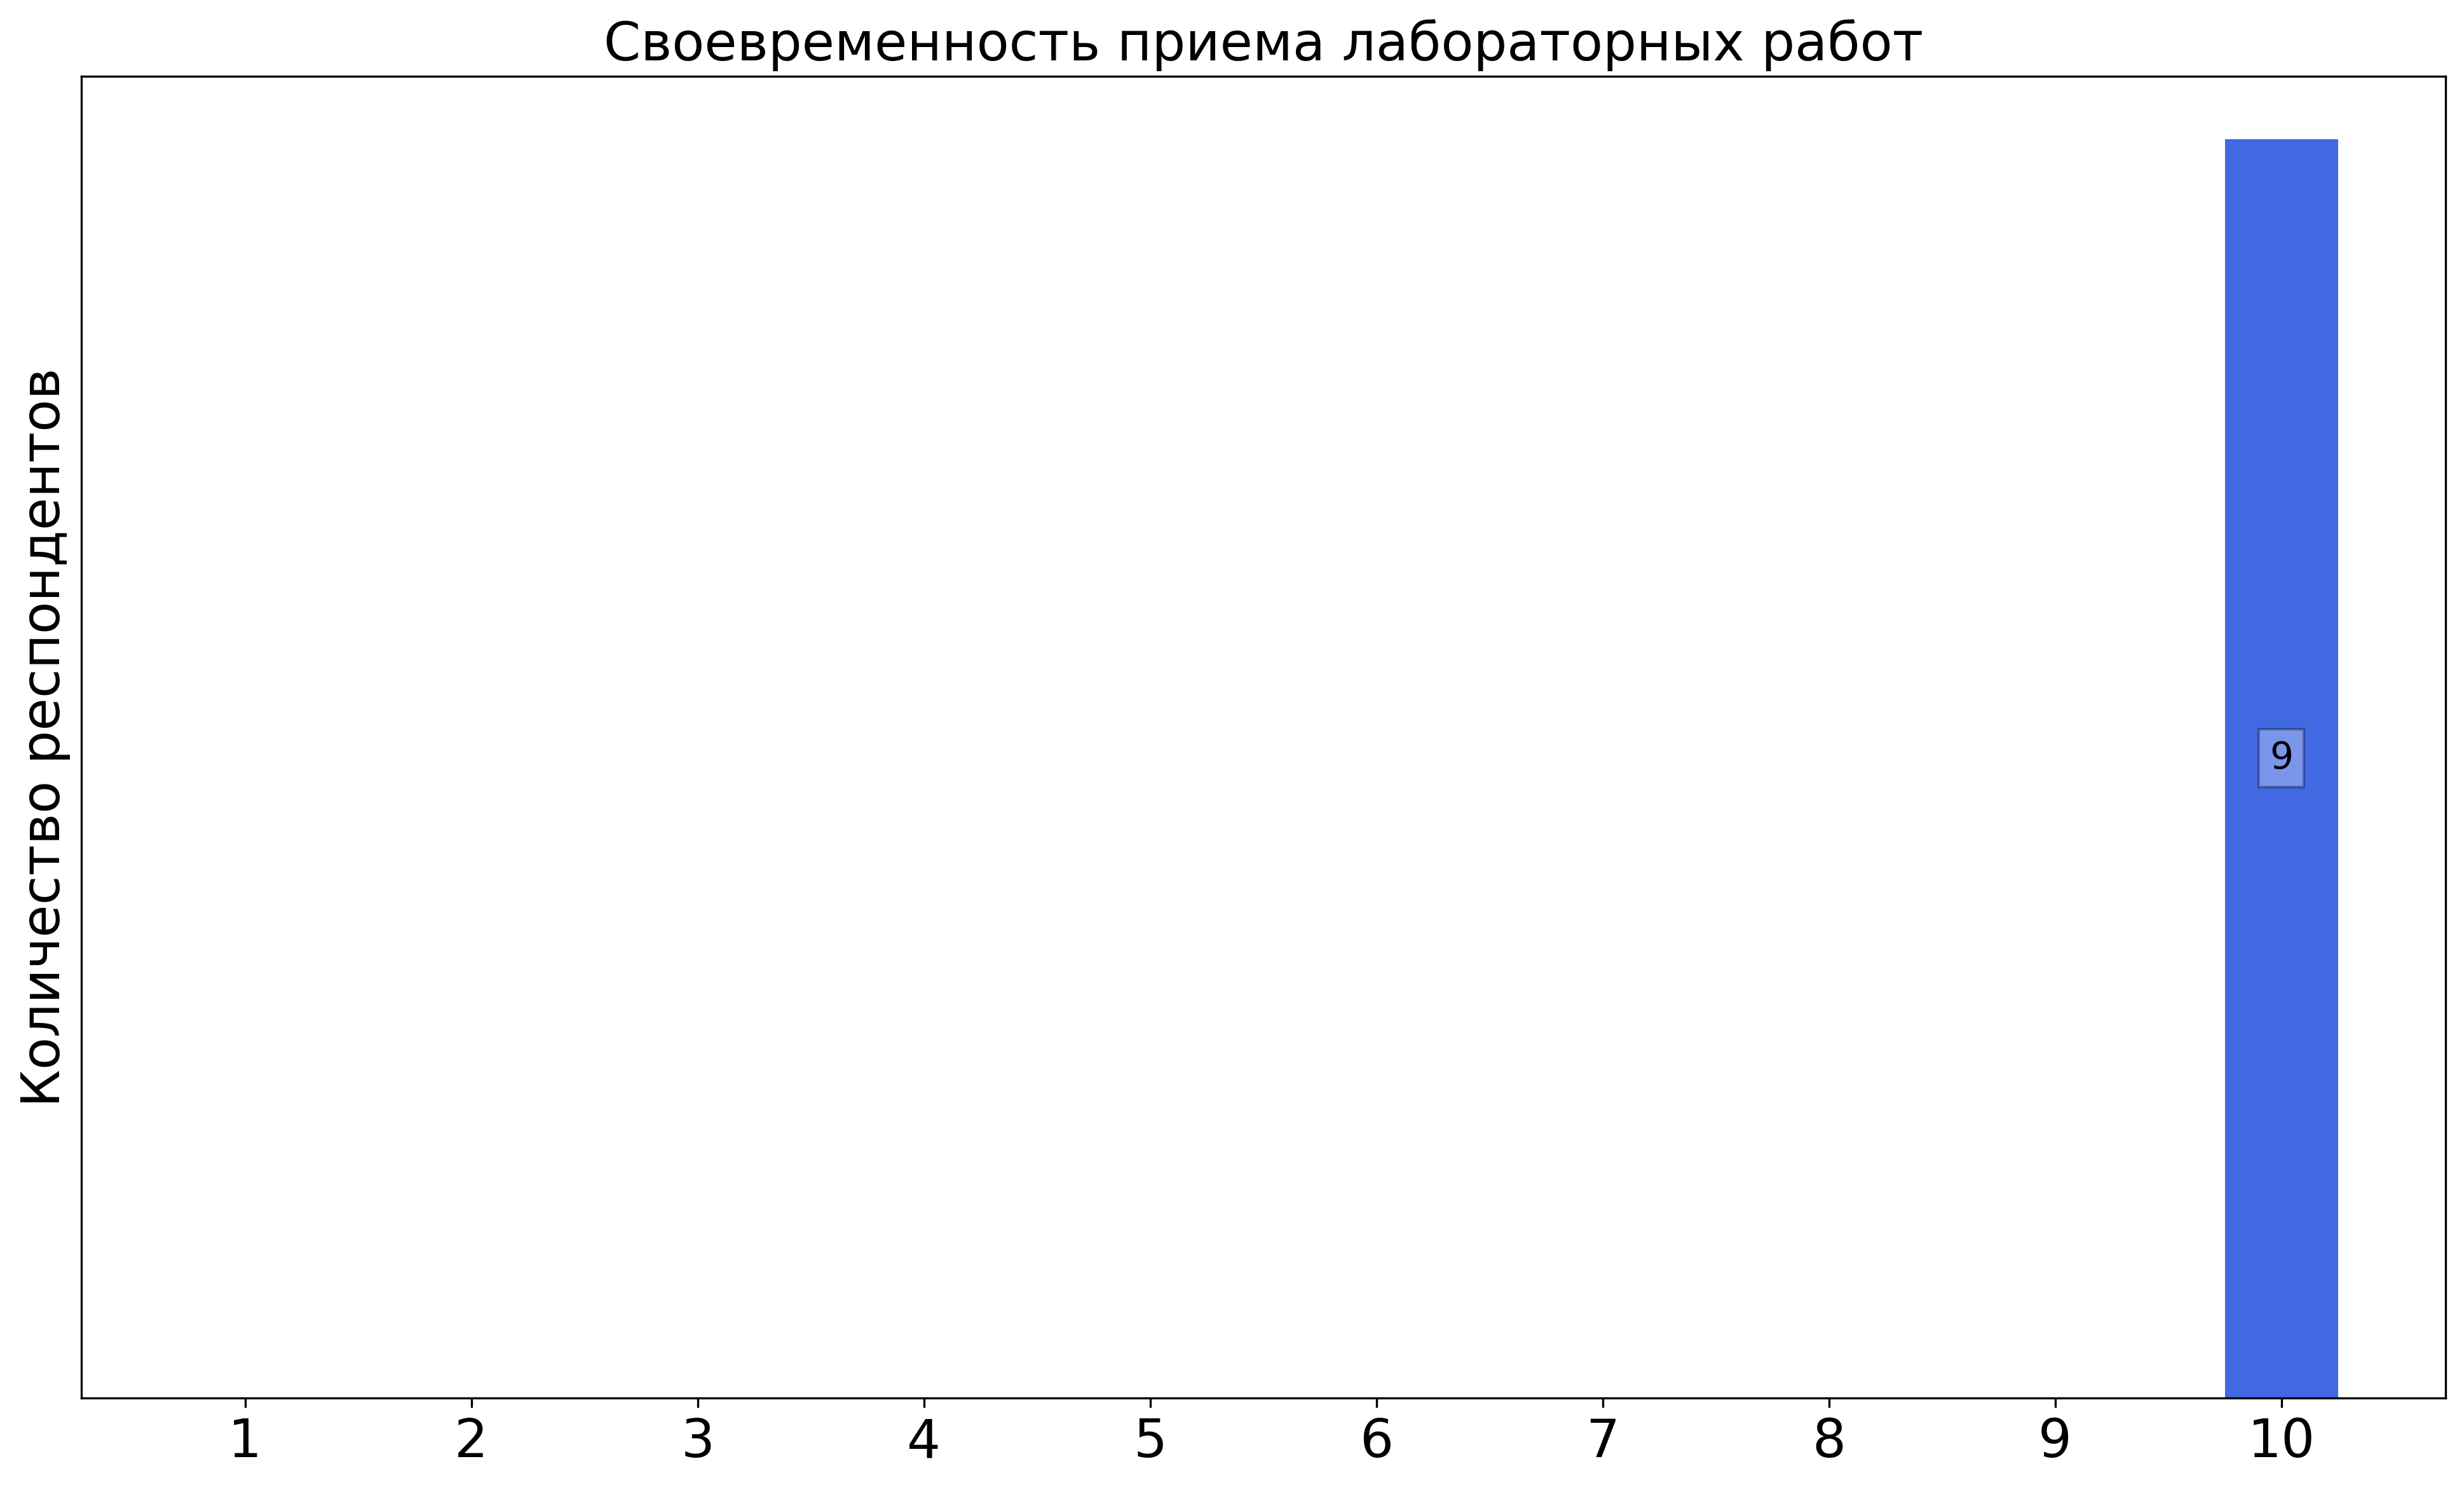
\includegraphics[width=\textwidth]{images/3 course/Радиофизическая лаборатория/labniks-marks-Борисов Д.А.-2.png}
            \end{subfigure}
            \begin{subfigure}[b]{0.45\textwidth}
                \centering
                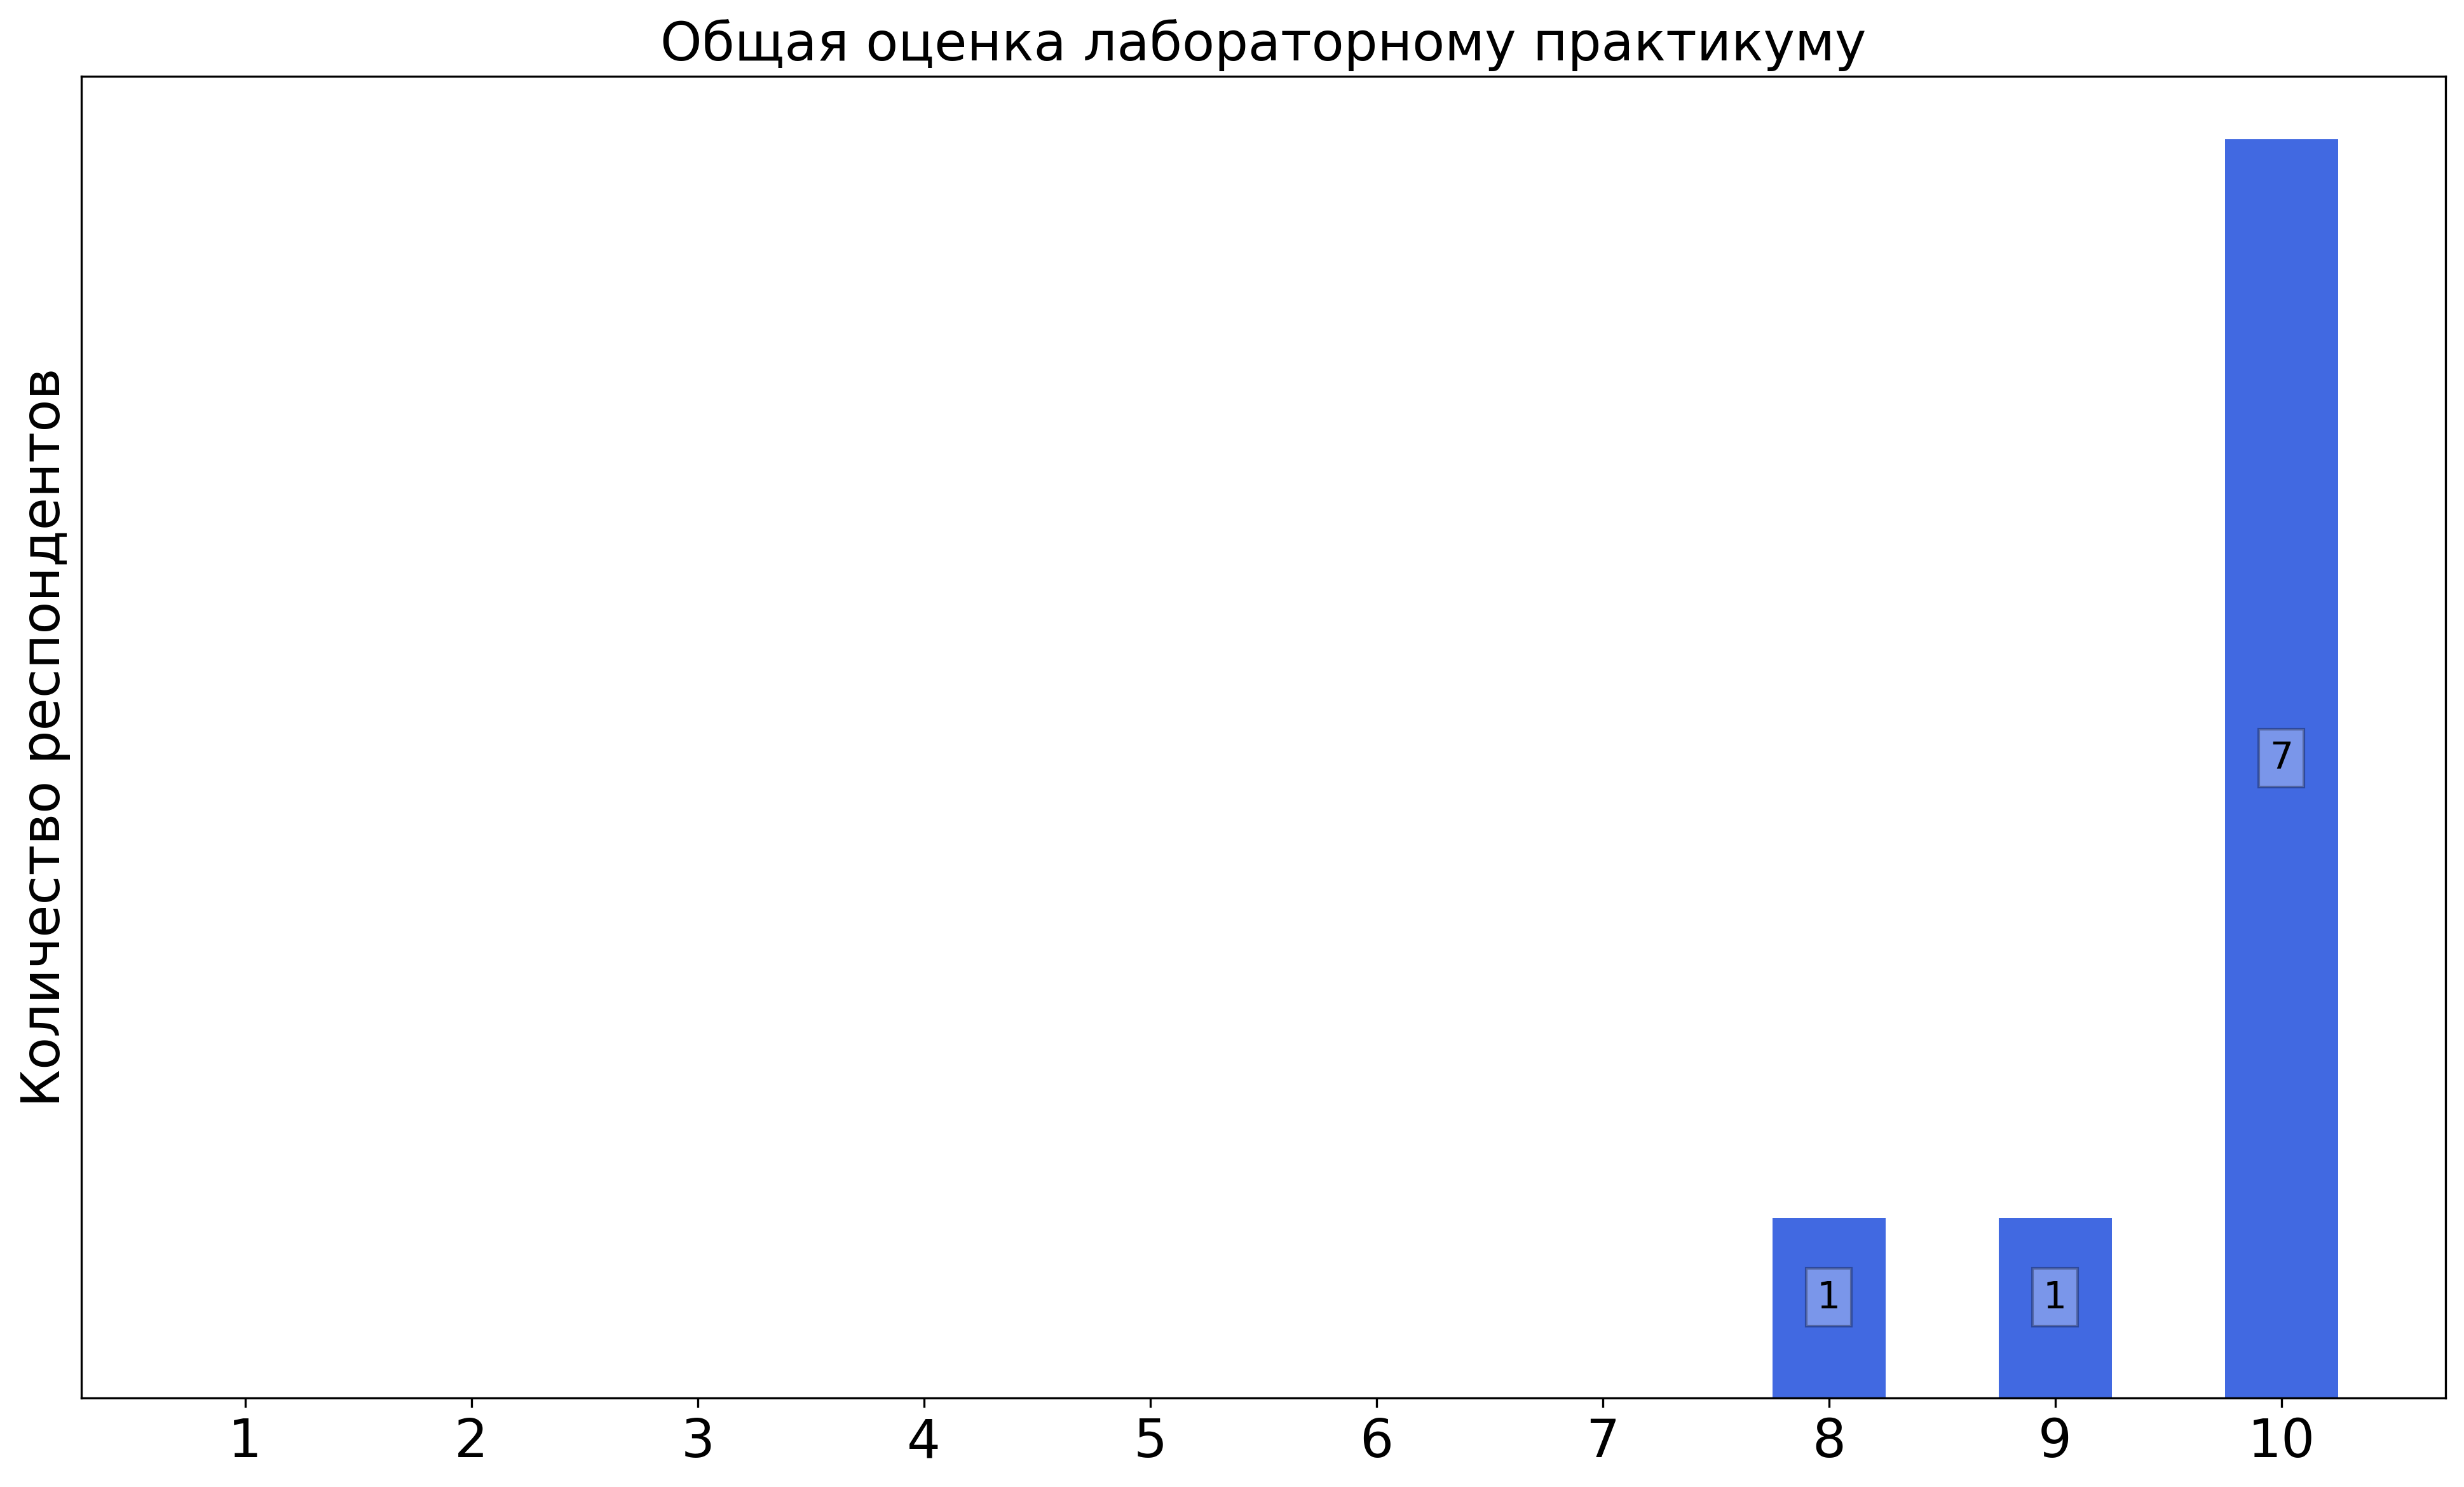
\includegraphics[width=\textwidth]{images/3 course/Радиофизическая лаборатория/labniks-marks-Борисов Д.А.-3.png}
            \end{subfigure}	
            \caption{Оценки респондентов о качестве преподавания лабораторных работ}
        \end{figure}

        \textbf{Комментарии студентов о преподавателе\protect\footnote{сохранены оригинальные орфография и пунктуация}}
            \begin{commentbox} 
                Преподаватель хороший, добрый, рассказывает нормально, на вопросы отвечает и объясняет

                Зачем этот предмет? Абсолютно бесполезный как будто 
            \end{commentbox} 
        
            \begin{commentbox} 
                Очень приятный курс. Материалы написаны хорошо, всё самому можно разобрать. Преподаватели всегда помогали и объясняли, если что-то неясно 
            \end{commentbox} 
        
            \begin{commentbox} 
                Курс был мне интересен, однако это связано с тем, что он сильно перекликается с областью, которой занимается моя базовая кафедра. Я бы не сказал, что этот курс нужен большинству студентов ФРКТ, лучше бы он оставался обязательным только для студентов кафедр смежных областей. Сами лабораторные работы велись хорошо, преподаватели всегда понятно излагали материал и помогали в случае возникновения трудностей с выполнением задания. 
            \end{commentbox} 
        
            \begin{commentbox} 
                Приятный курс, приятный преподаватель 
            \end{commentbox}

    \subsubsection{Отзыв студентов о лабораторных работах. Преподаватель: Водичев Н.А.}
        \begin{figure}[H]
            \centering
            \begin{subfigure}[b]{0.45\textwidth}
                \centering
                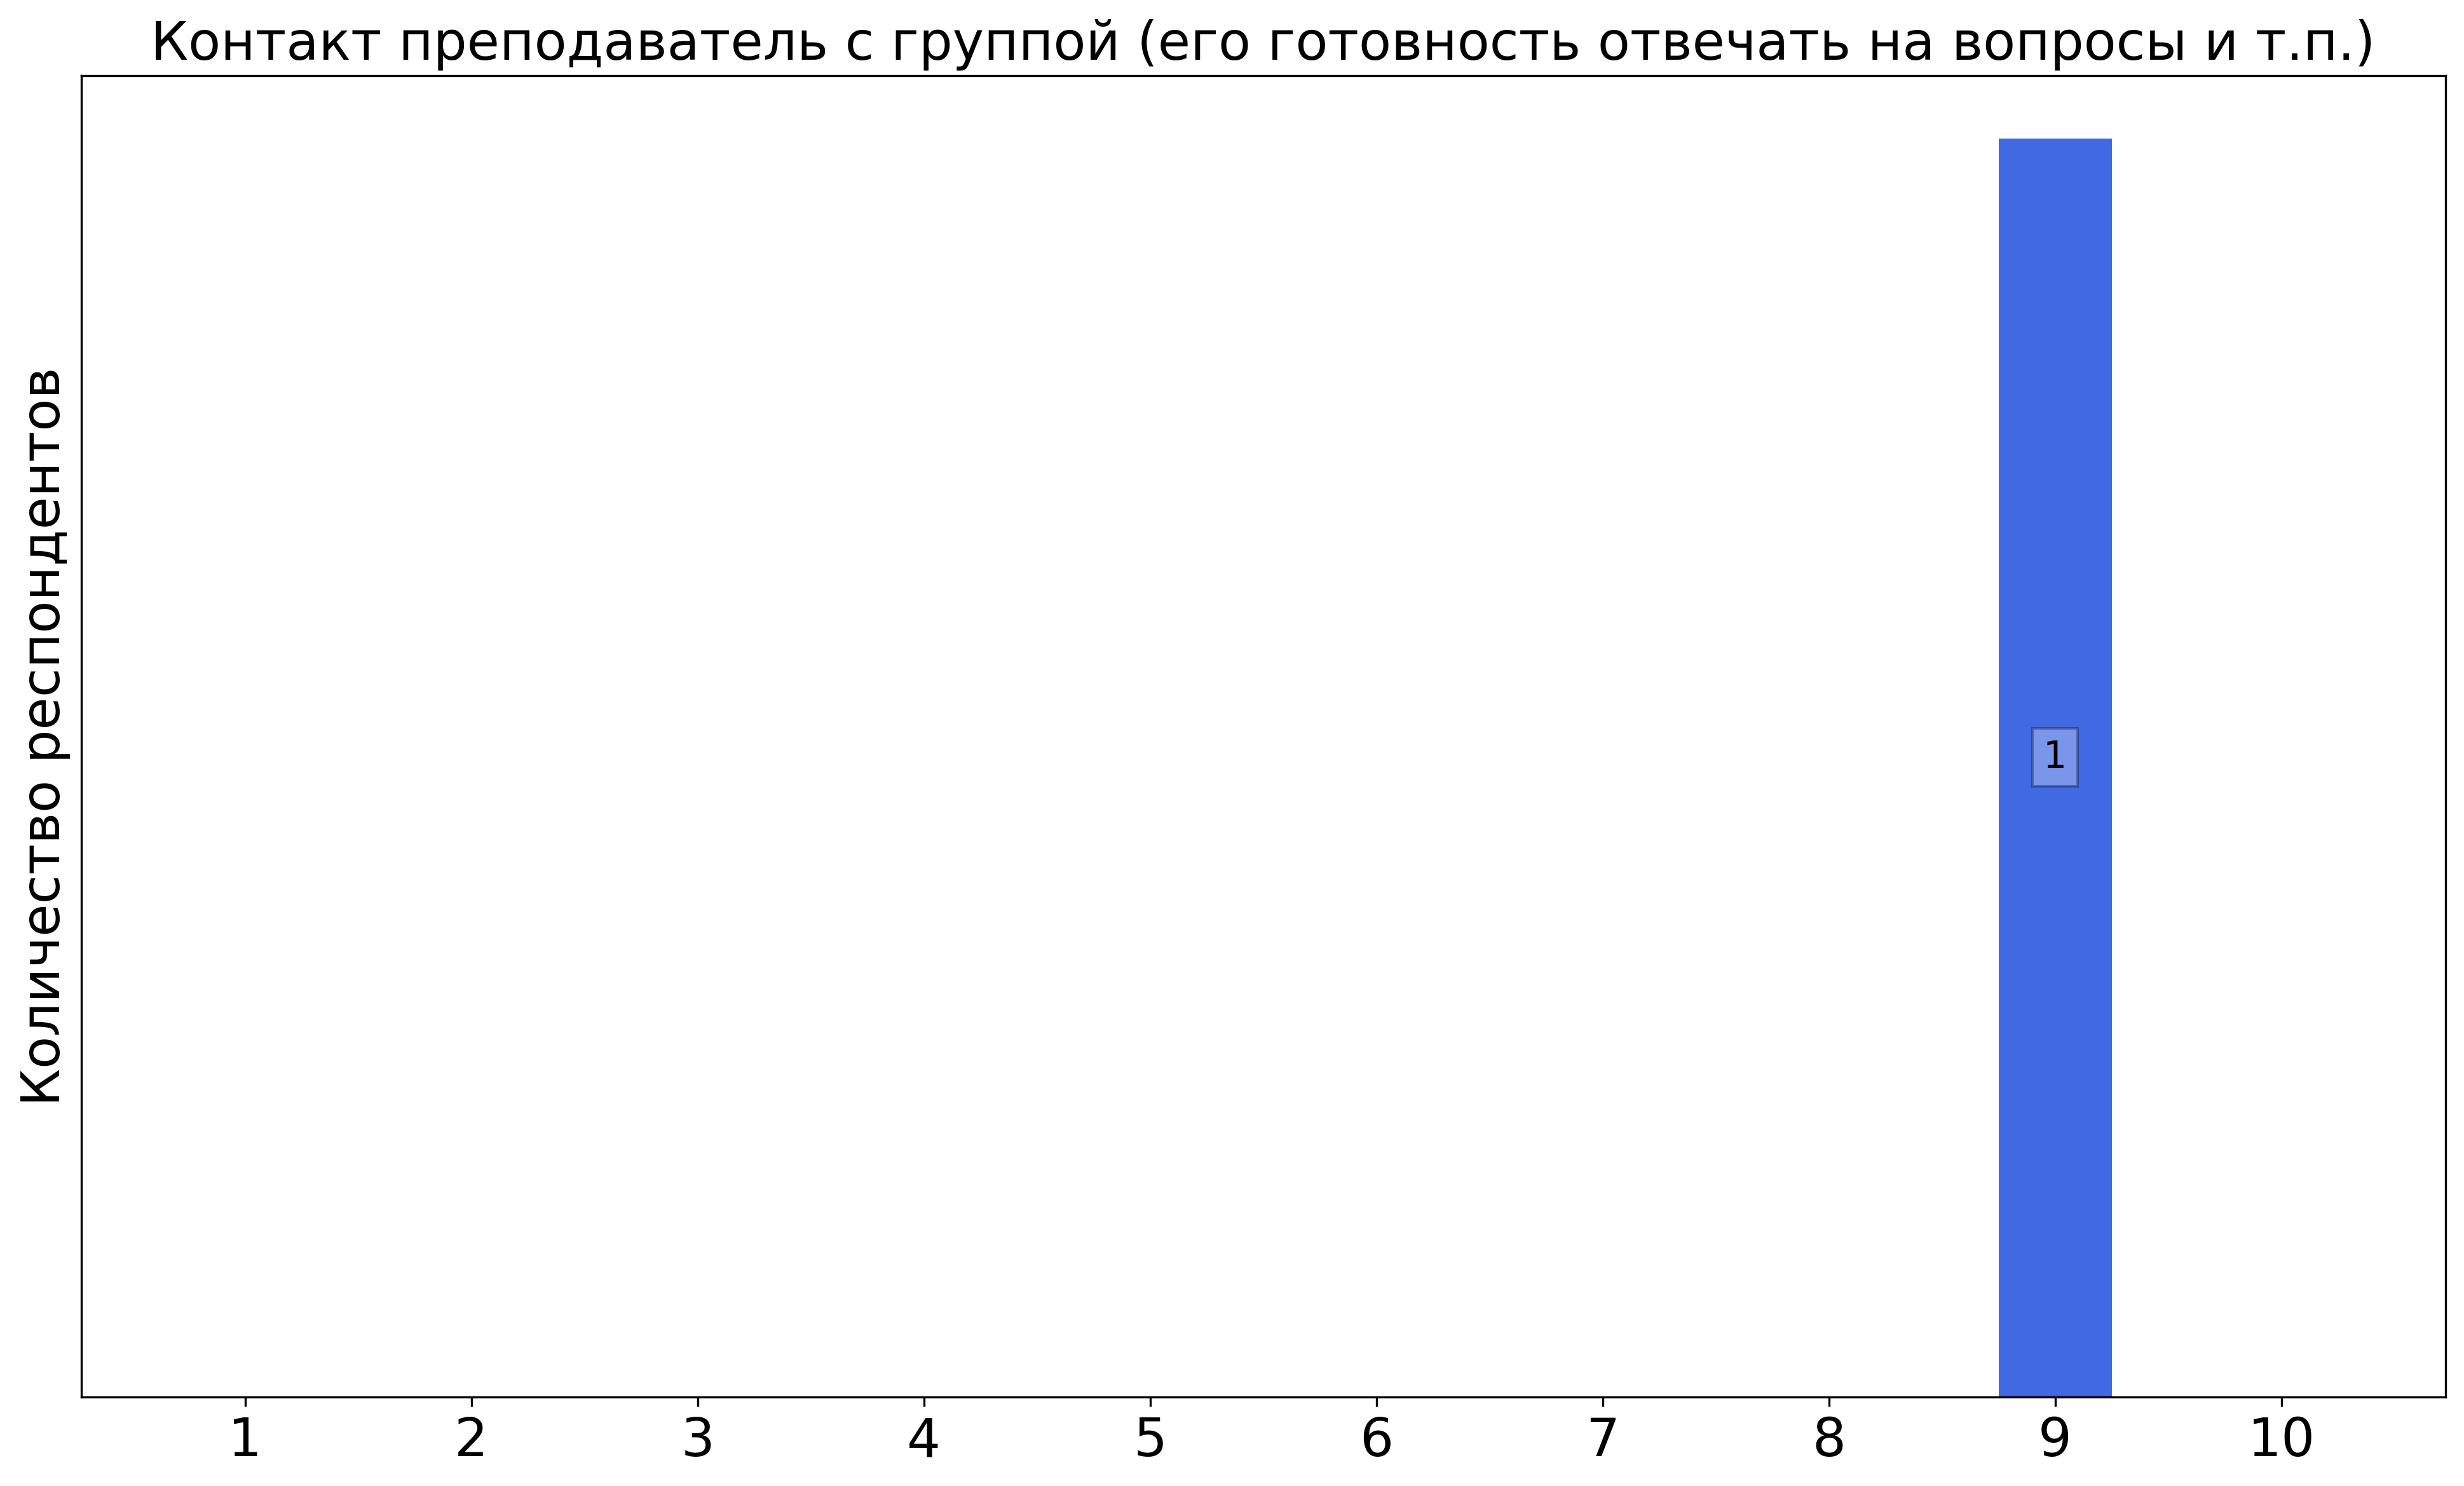
\includegraphics[width=\textwidth]{images/3 course/Радиофизическая лаборатория/labniks-marks-Водичев Н.А.-0.png}
            \end{subfigure}
            \begin{subfigure}[b]{0.45\textwidth}
                \centering
                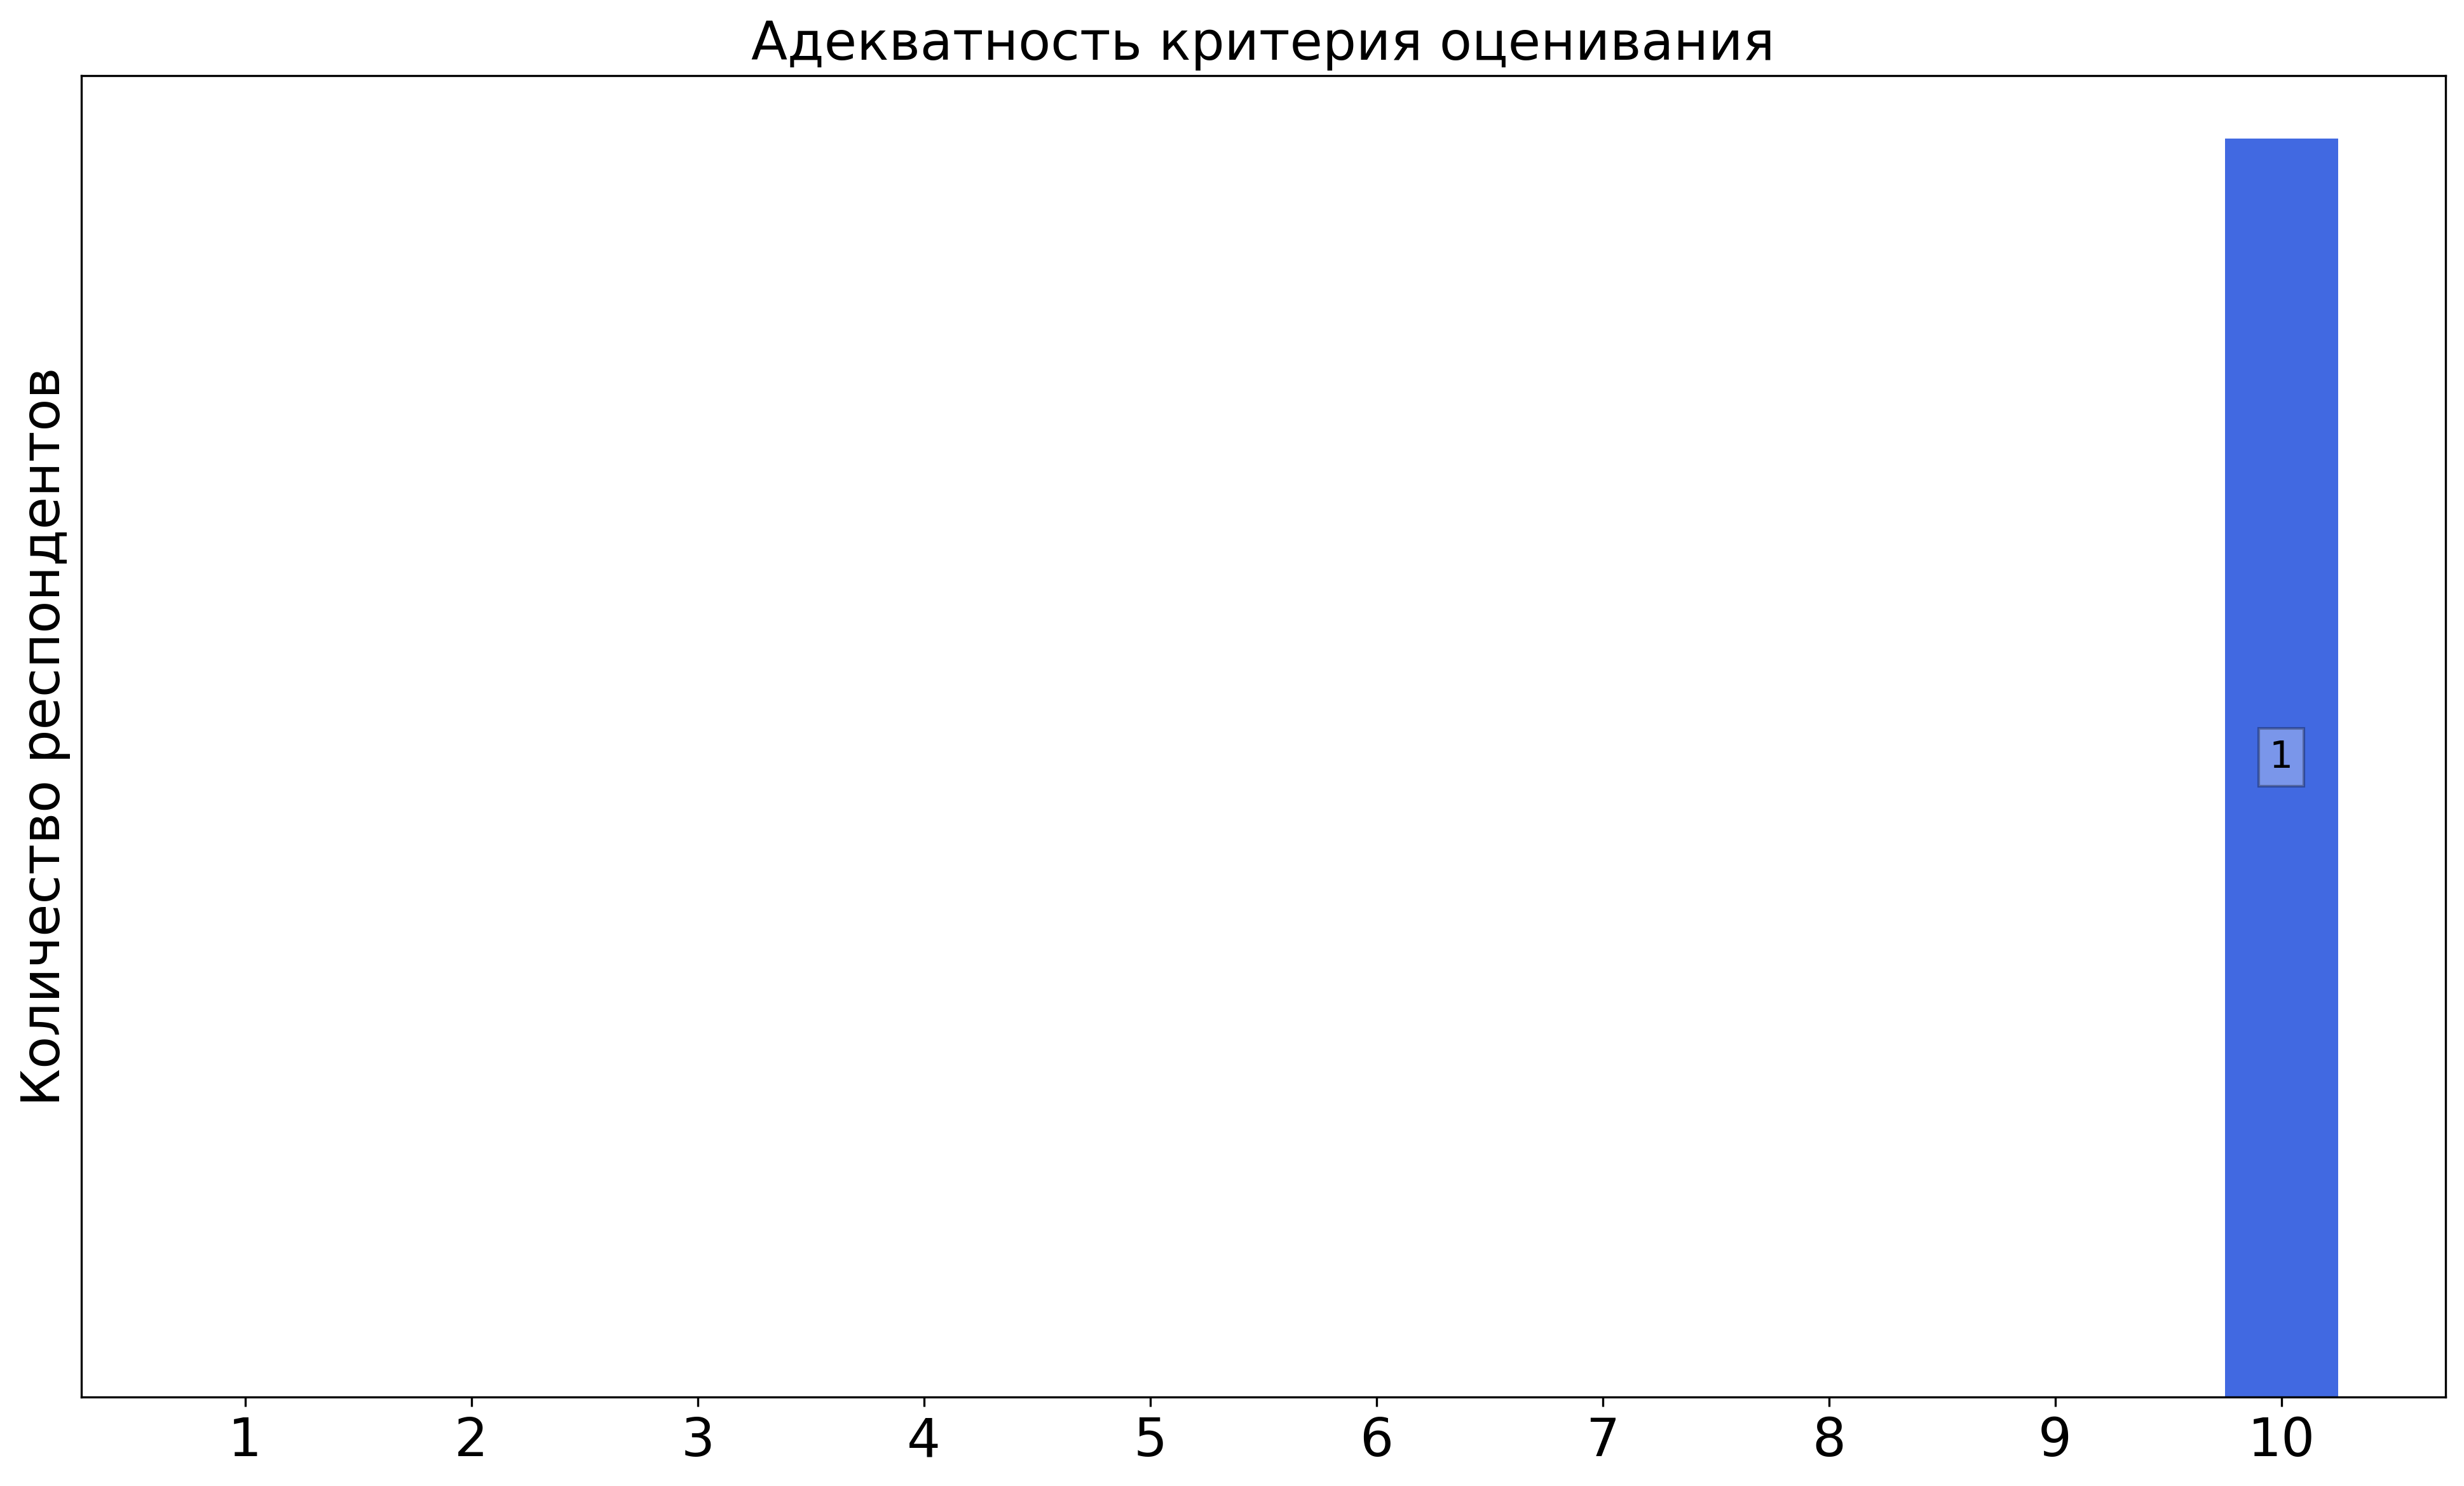
\includegraphics[width=\textwidth]{images/3 course/Радиофизическая лаборатория/labniks-marks-Водичев Н.А.-1.png}
            \end{subfigure}
            \begin{subfigure}[b]{0.45\textwidth}
                \centering
                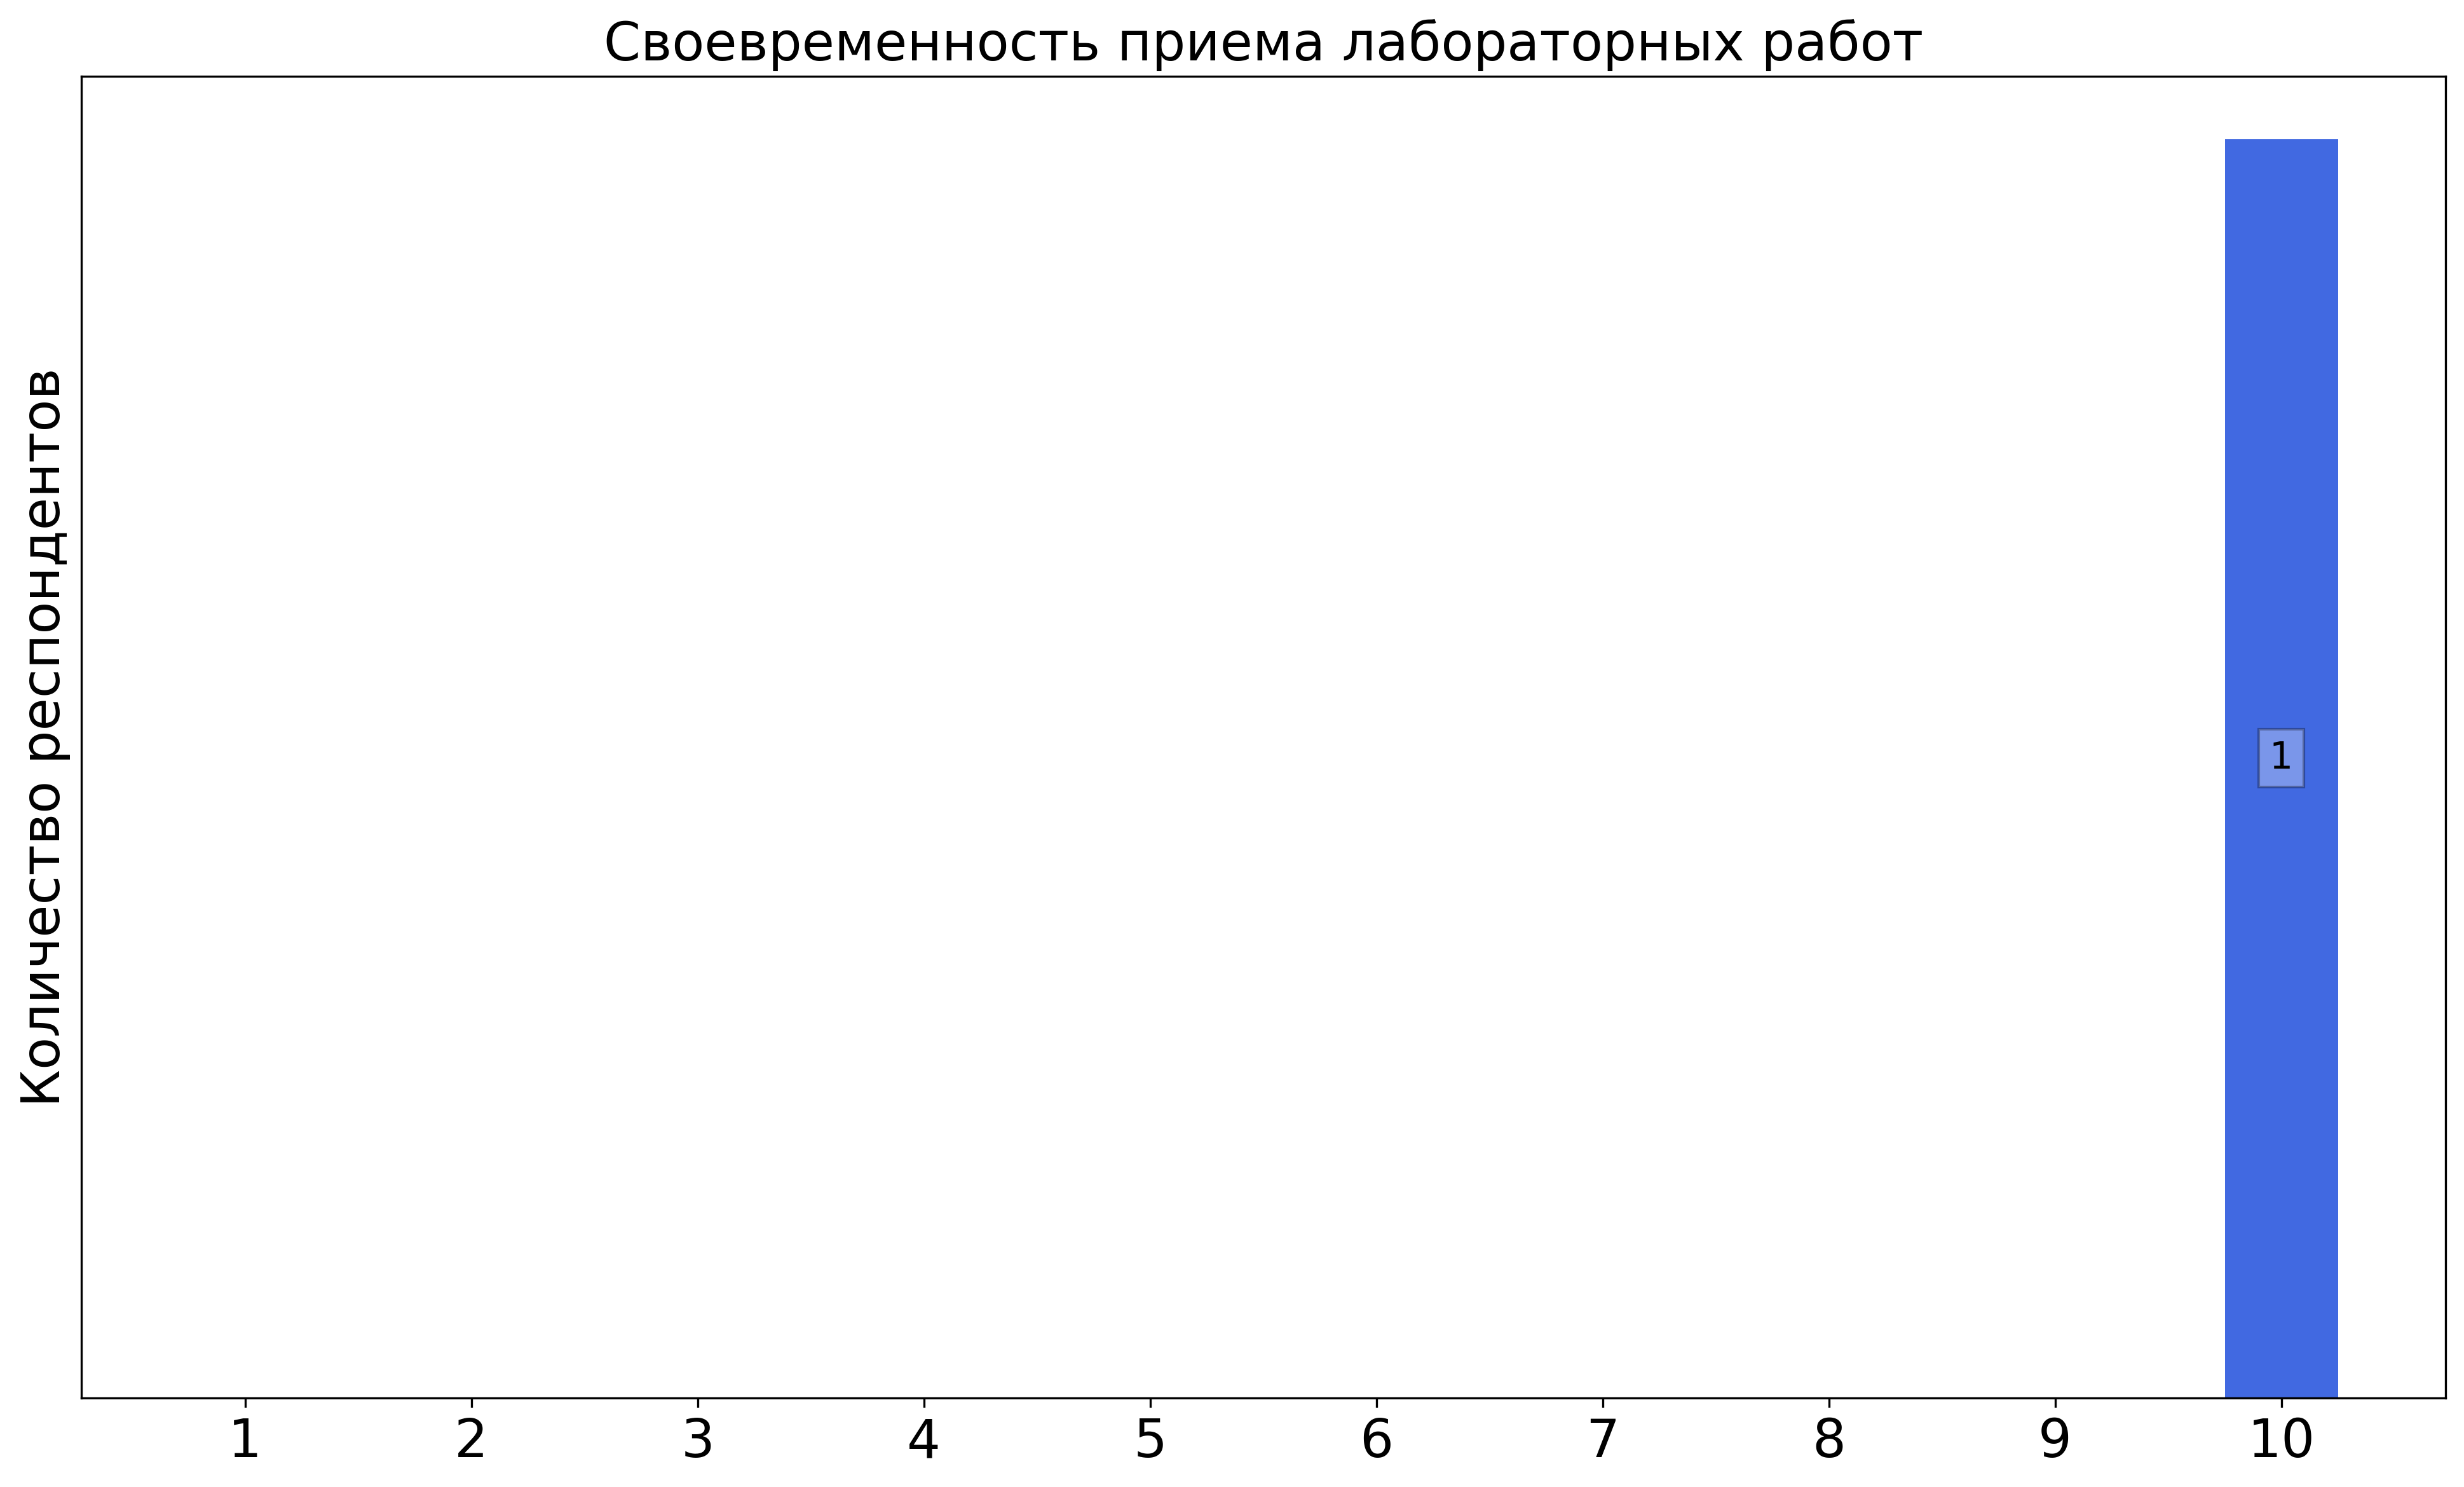
\includegraphics[width=\textwidth]{images/3 course/Радиофизическая лаборатория/labniks-marks-Водичев Н.А.-2.png}
            \end{subfigure}
            \begin{subfigure}[b]{0.45\textwidth}
                \centering
                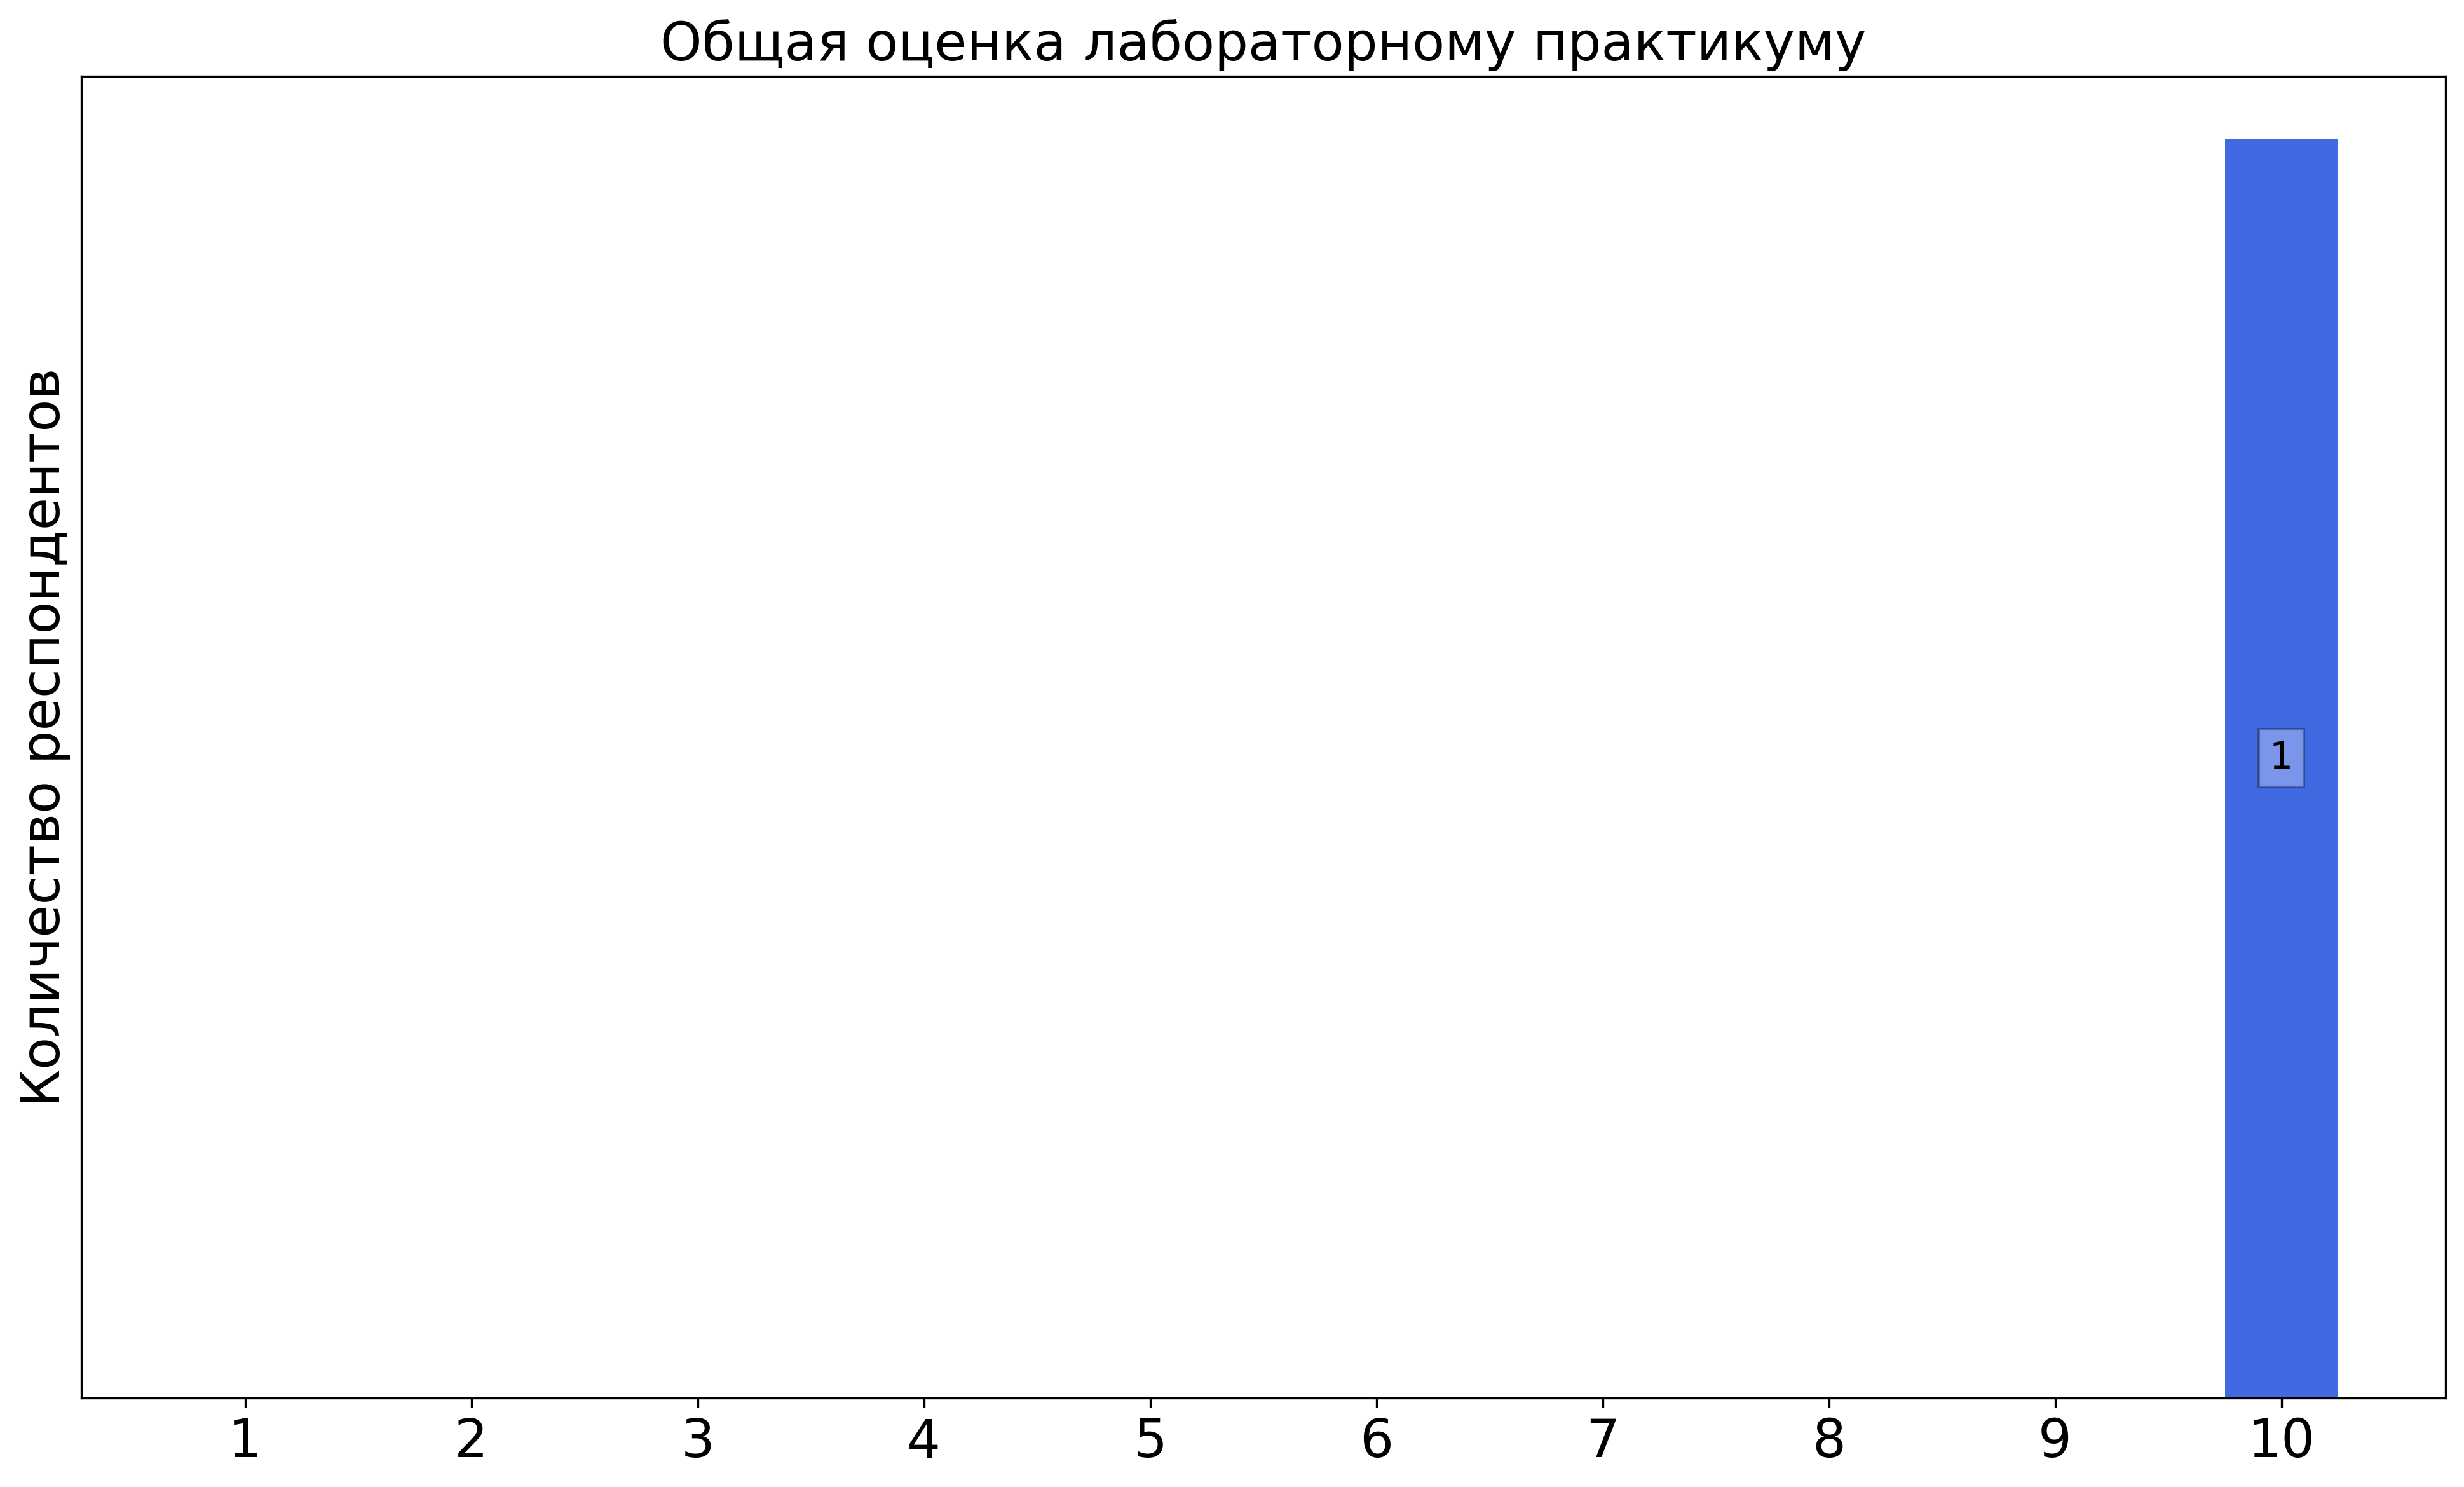
\includegraphics[width=\textwidth]{images/3 course/Радиофизическая лаборатория/labniks-marks-Водичев Н.А.-3.png}
            \end{subfigure}	
            \caption{Оценки респондентов о качестве преподавания лабораторных работ}
        \end{figure}


    \subsubsection{Отзыв студентов о лабораторных работах. Преподаватель: Манукян В.К.}
		\begin{figure}[H]
			\centering
			\begin{subfigure}[b]{0.45\textwidth}
				\centering
				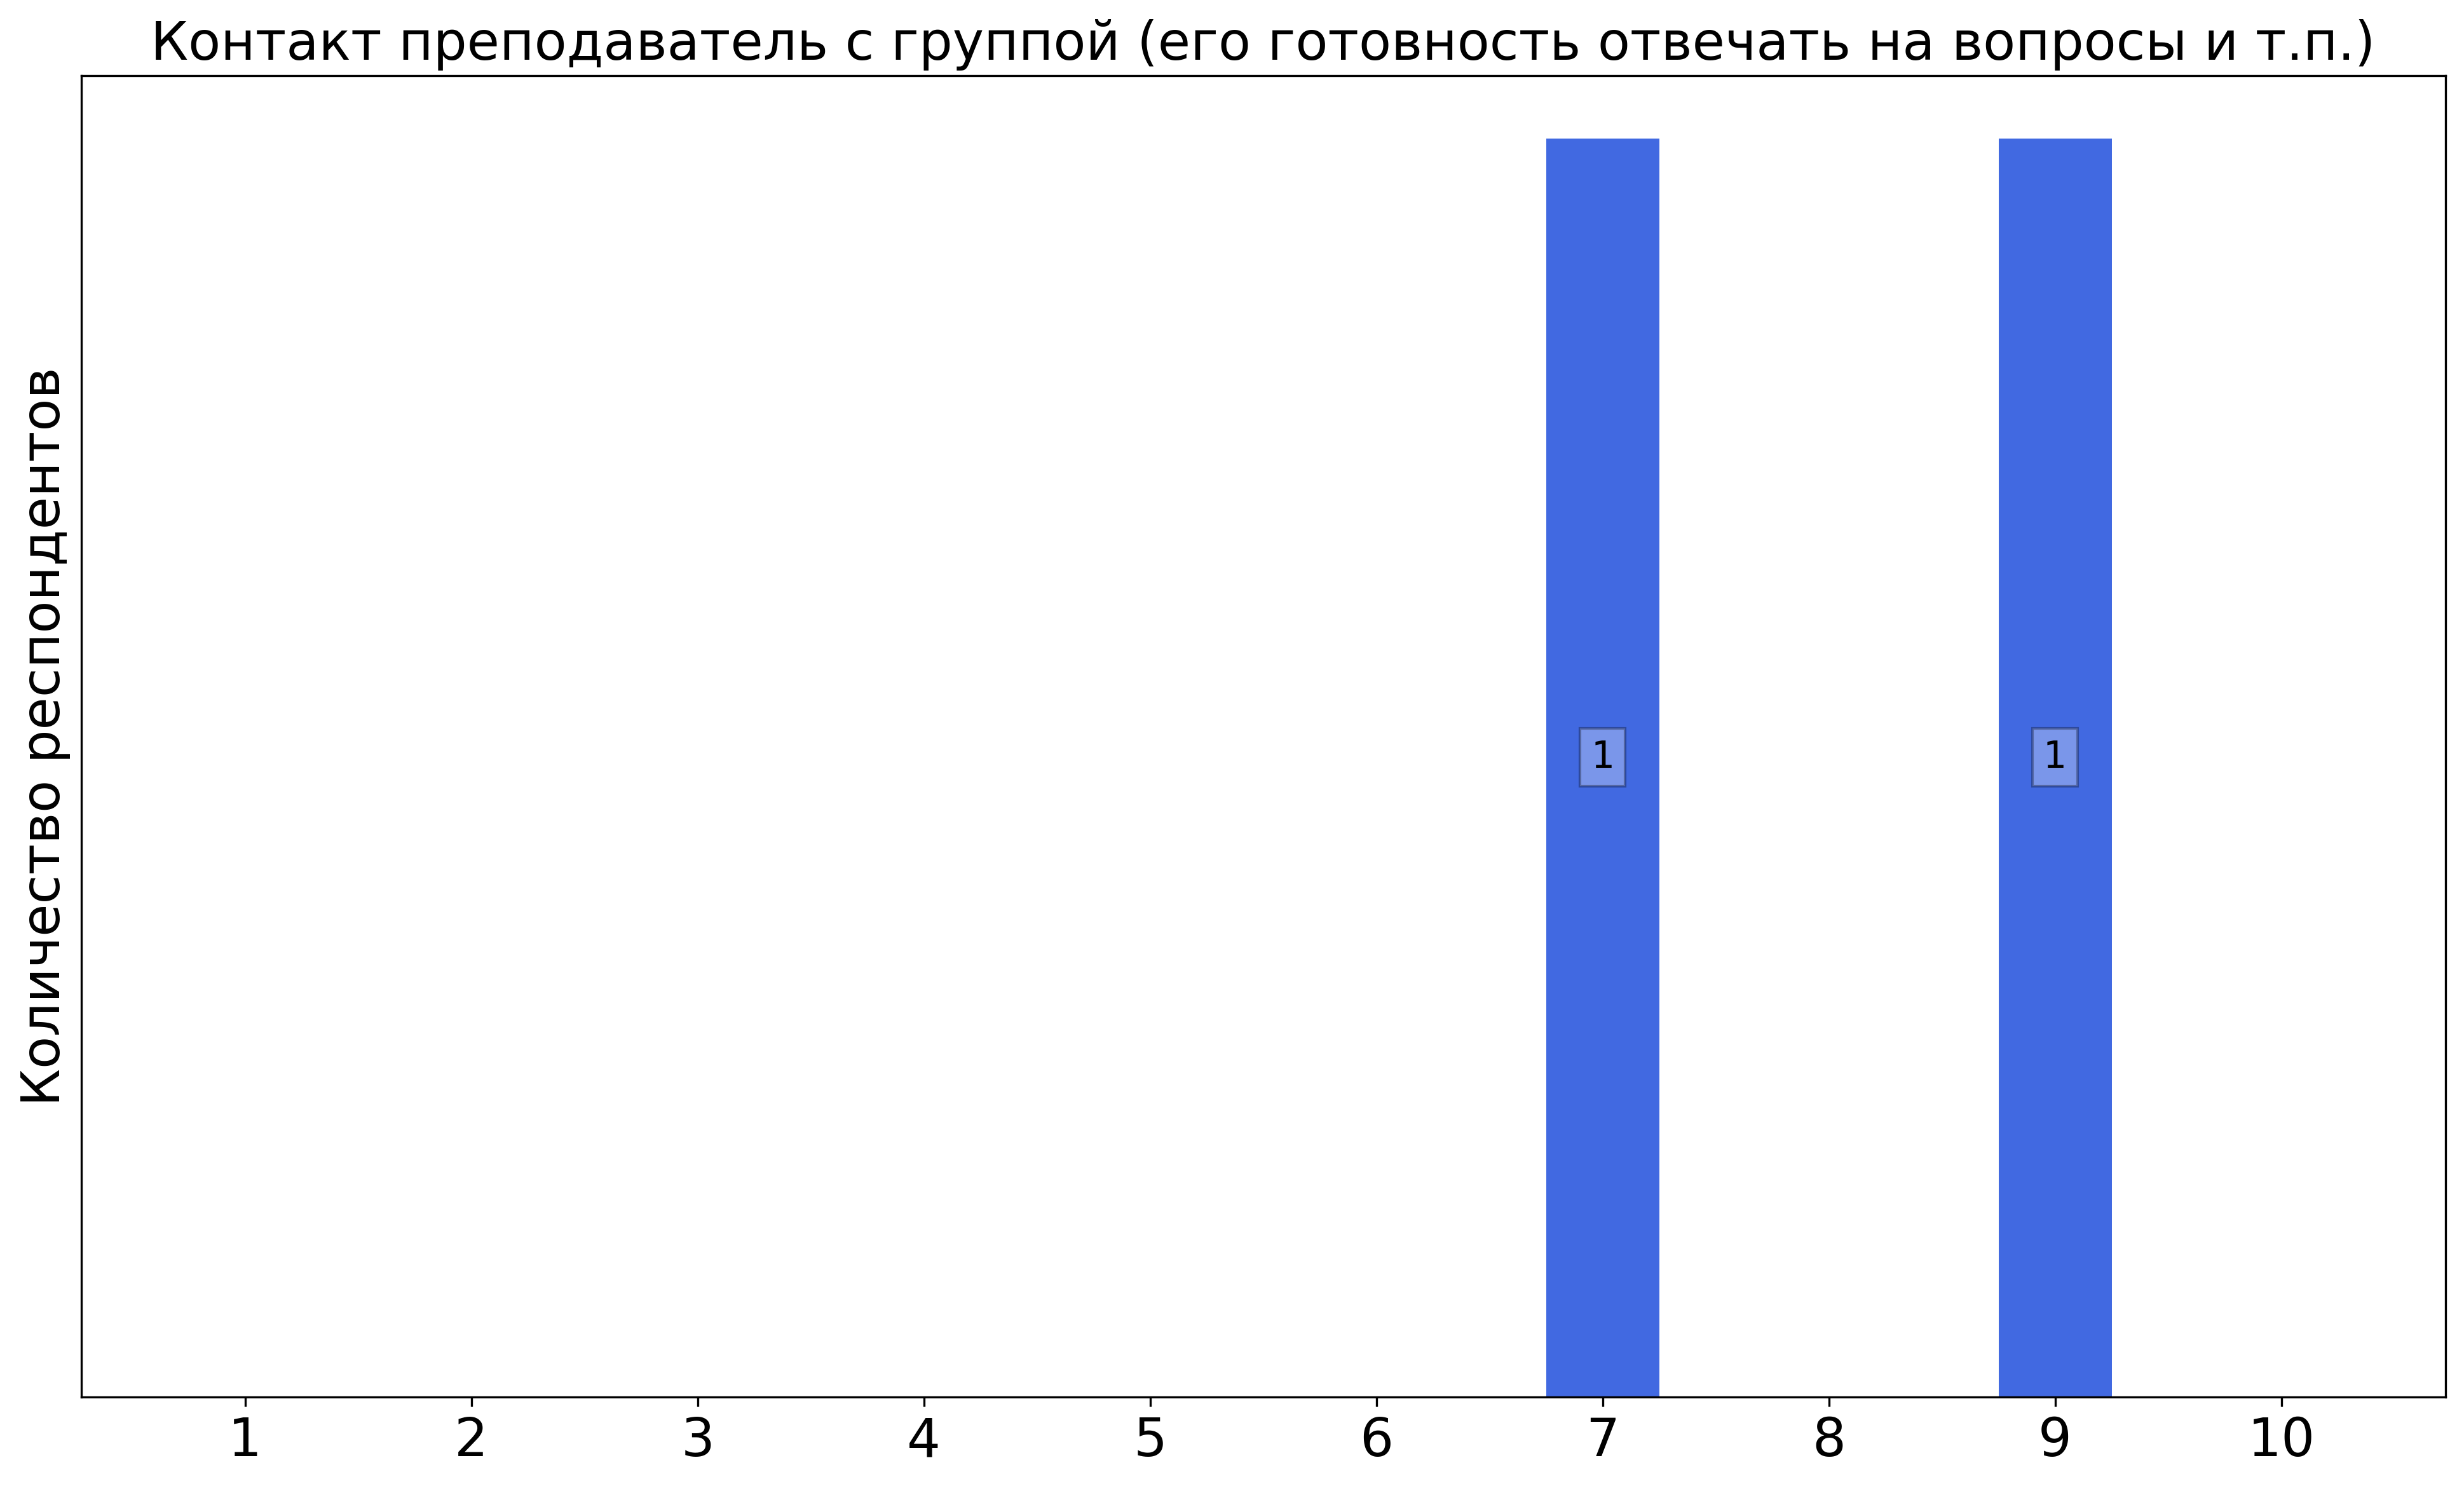
\includegraphics[width=\textwidth]{images/3 course/Радиофизическая лаборатория/labniks-marks-Манукян В.К.-0.png}
			\end{subfigure}
			\begin{subfigure}[b]{0.45\textwidth}
				\centering
				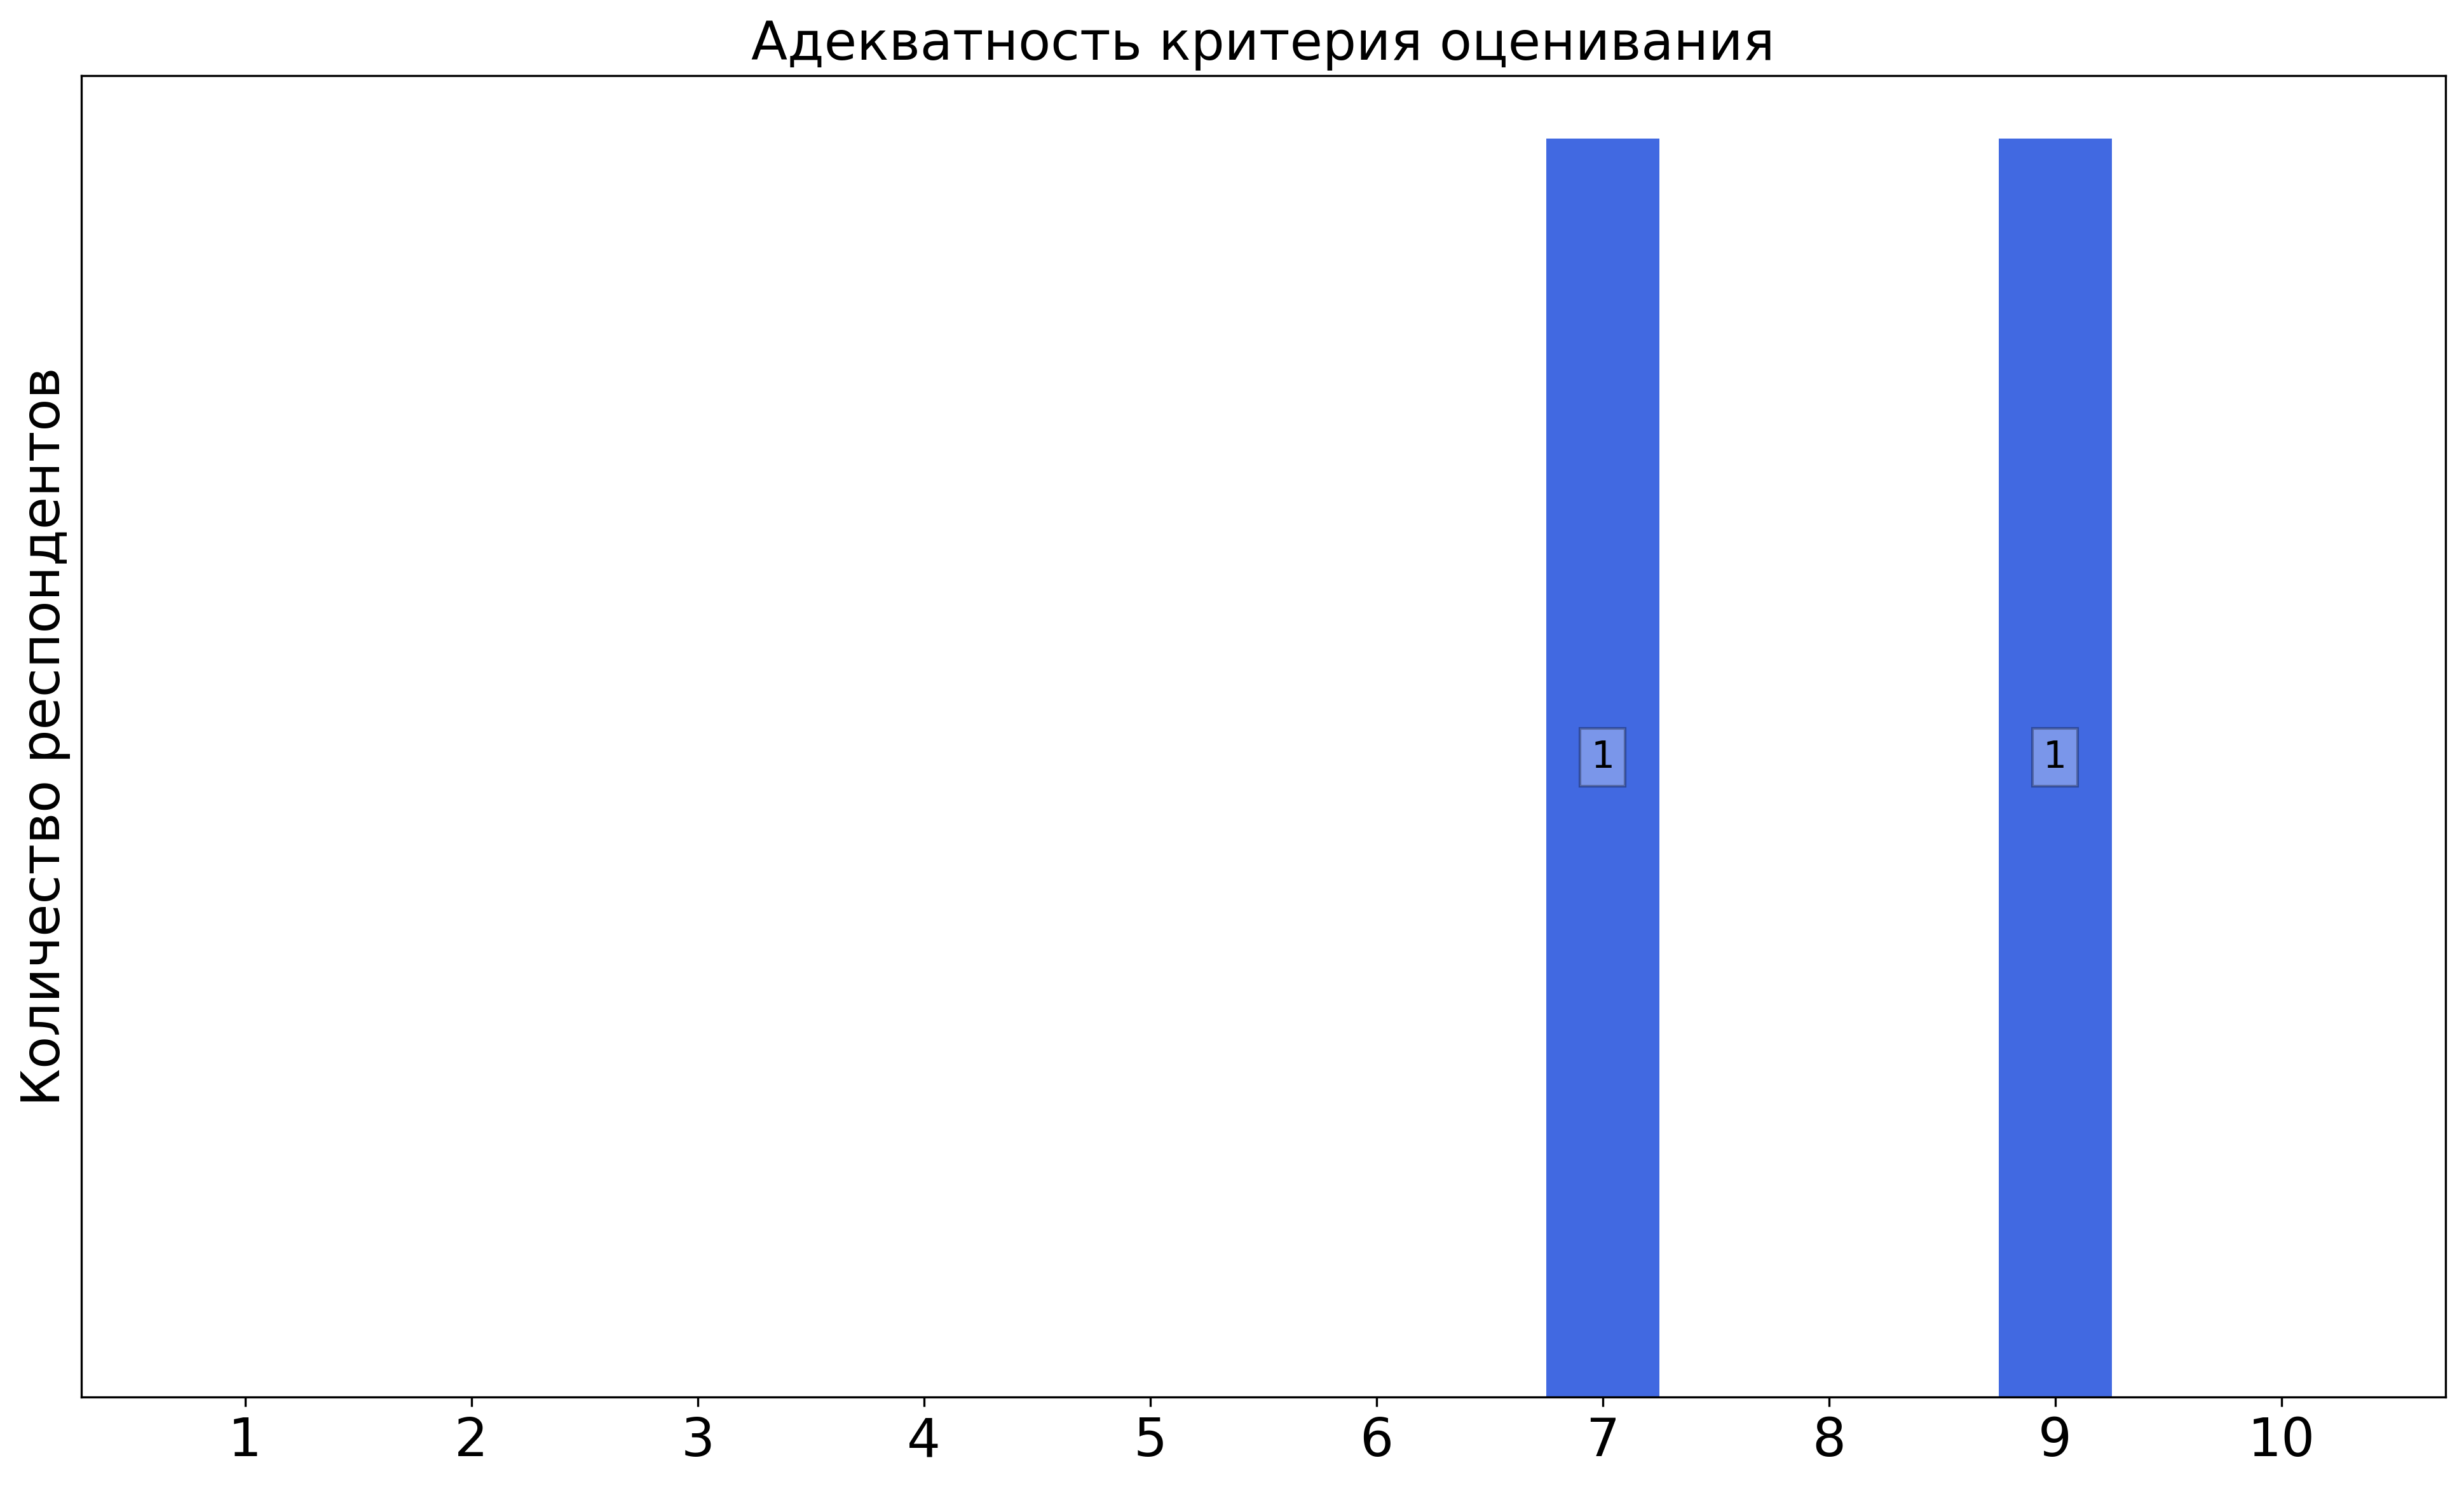
\includegraphics[width=\textwidth]{images/3 course/Радиофизическая лаборатория/labniks-marks-Манукян В.К.-1.png}
			\end{subfigure}
			\begin{subfigure}[b]{0.45\textwidth}
				\centering
				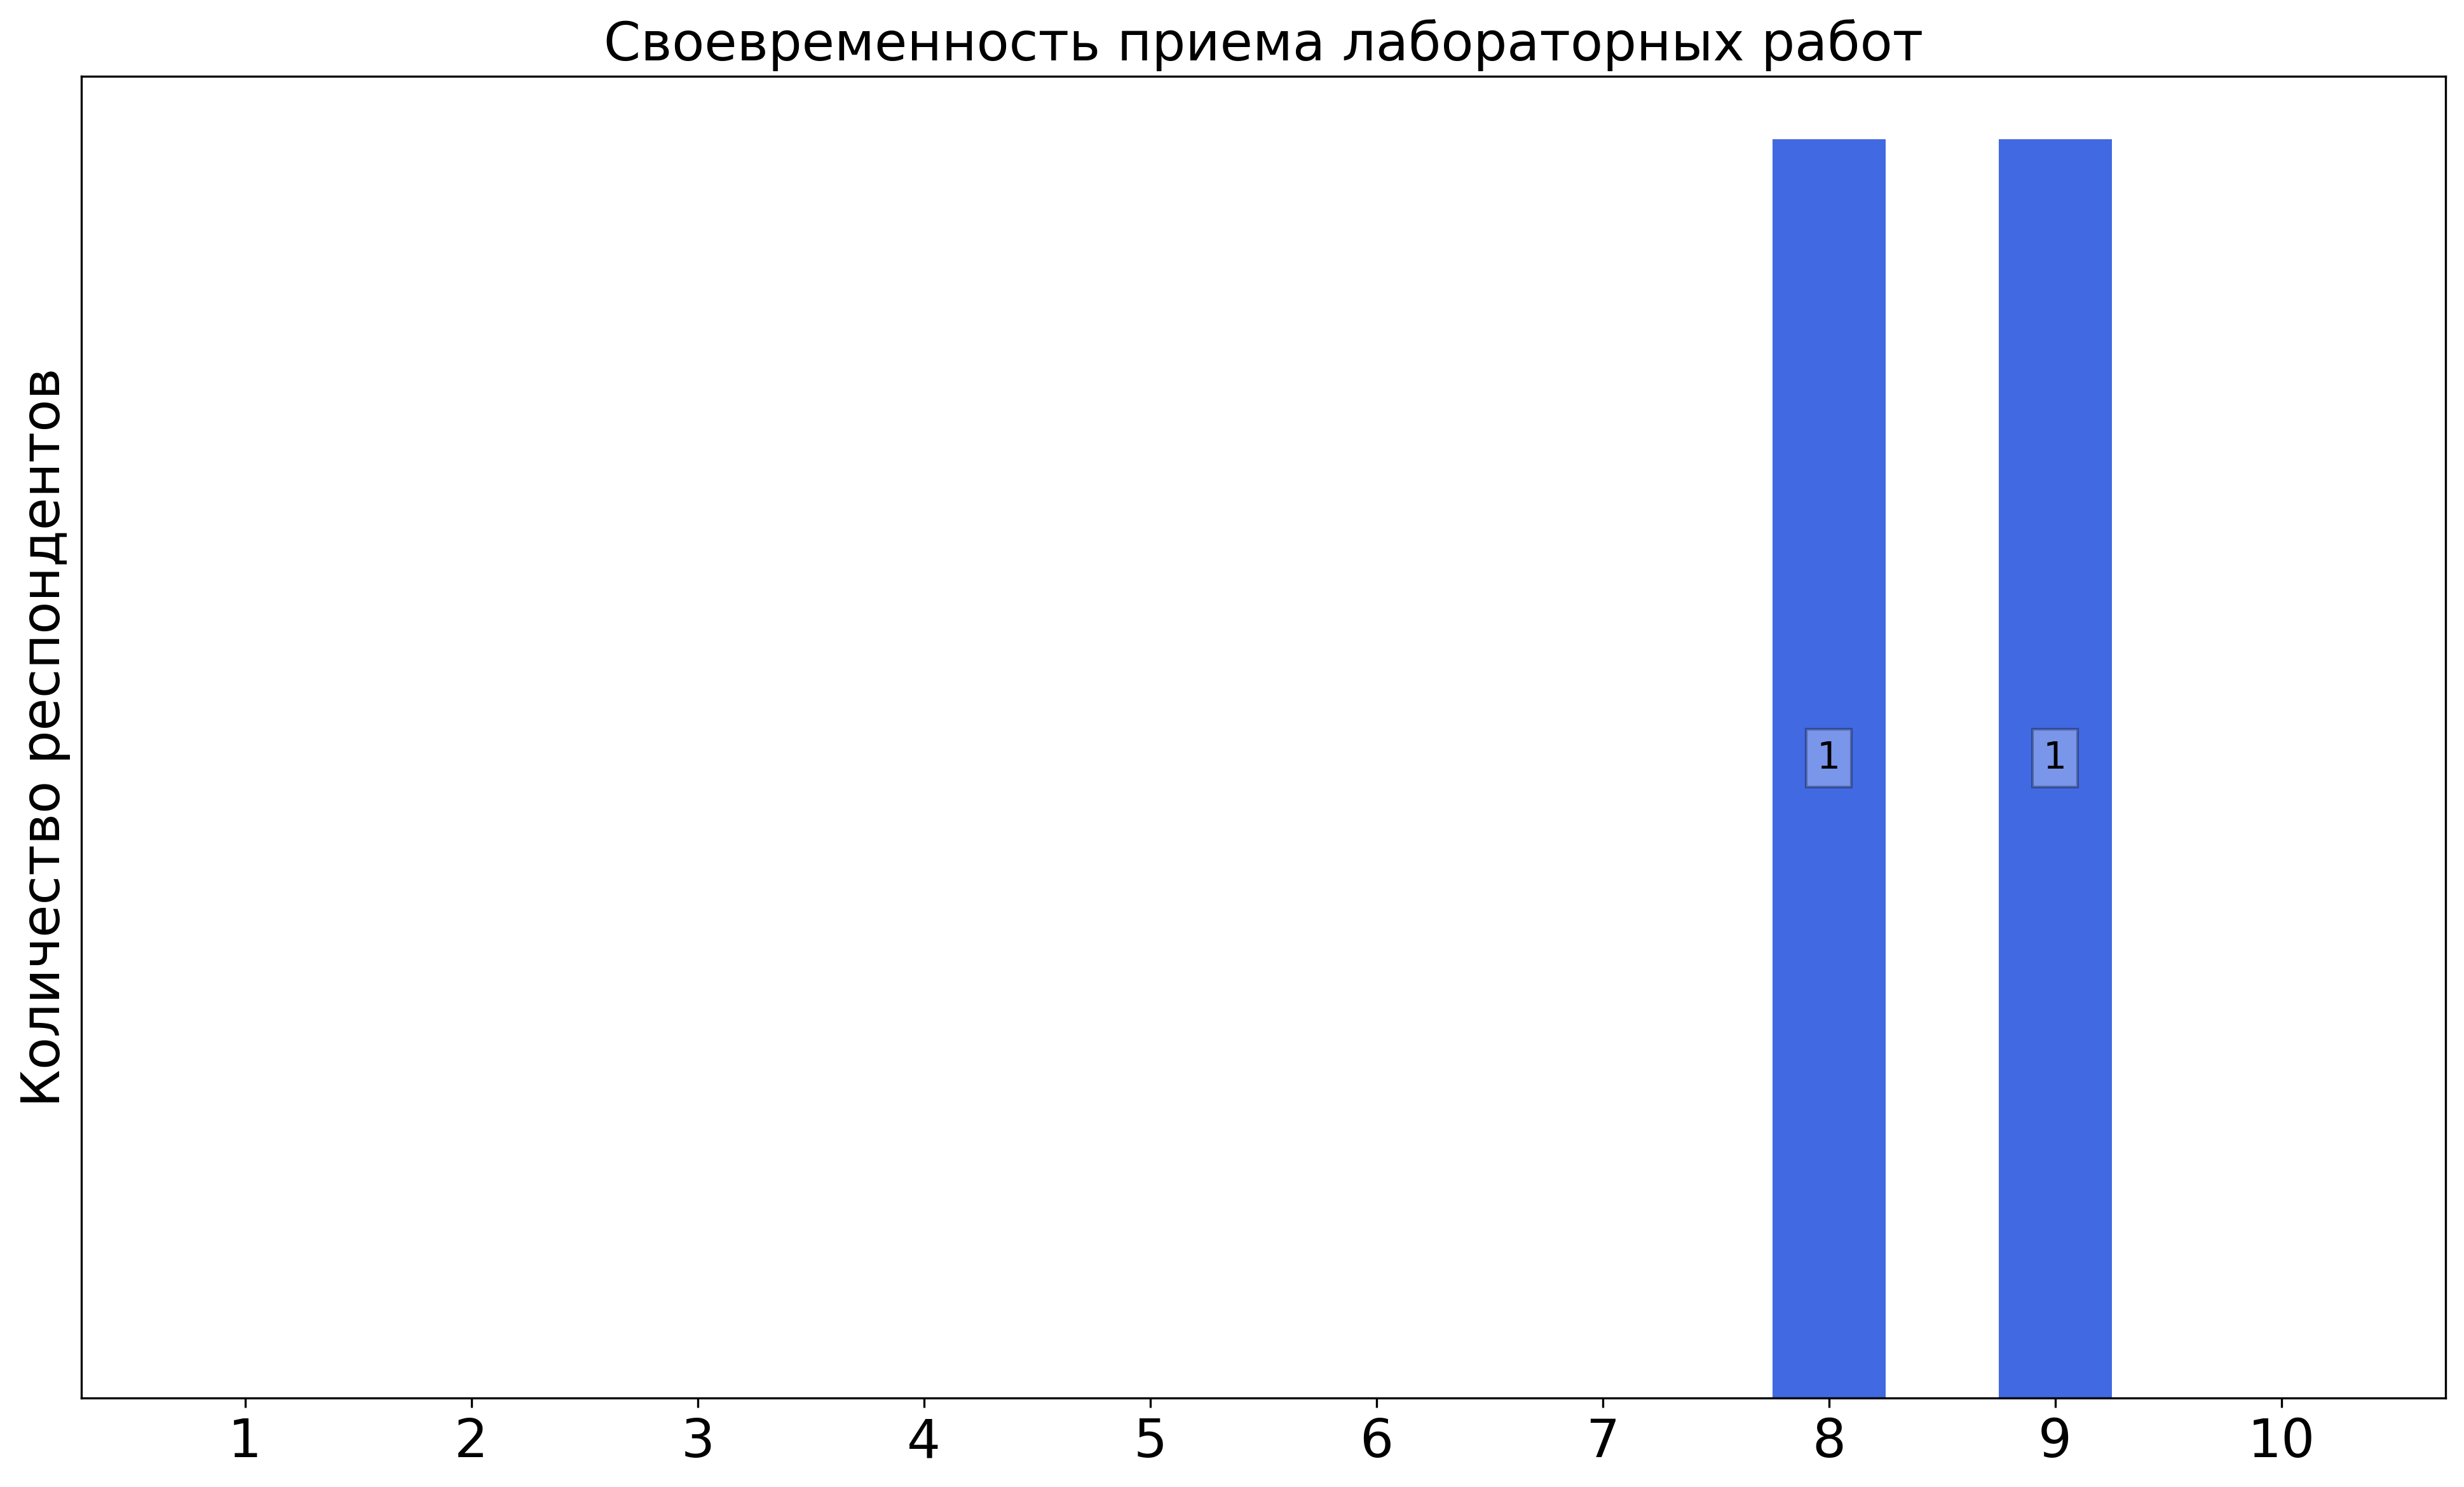
\includegraphics[width=\textwidth]{images/3 course/Радиофизическая лаборатория/labniks-marks-Манукян В.К.-2.png}
			\end{subfigure}
			\begin{subfigure}[b]{0.45\textwidth}
				\centering
				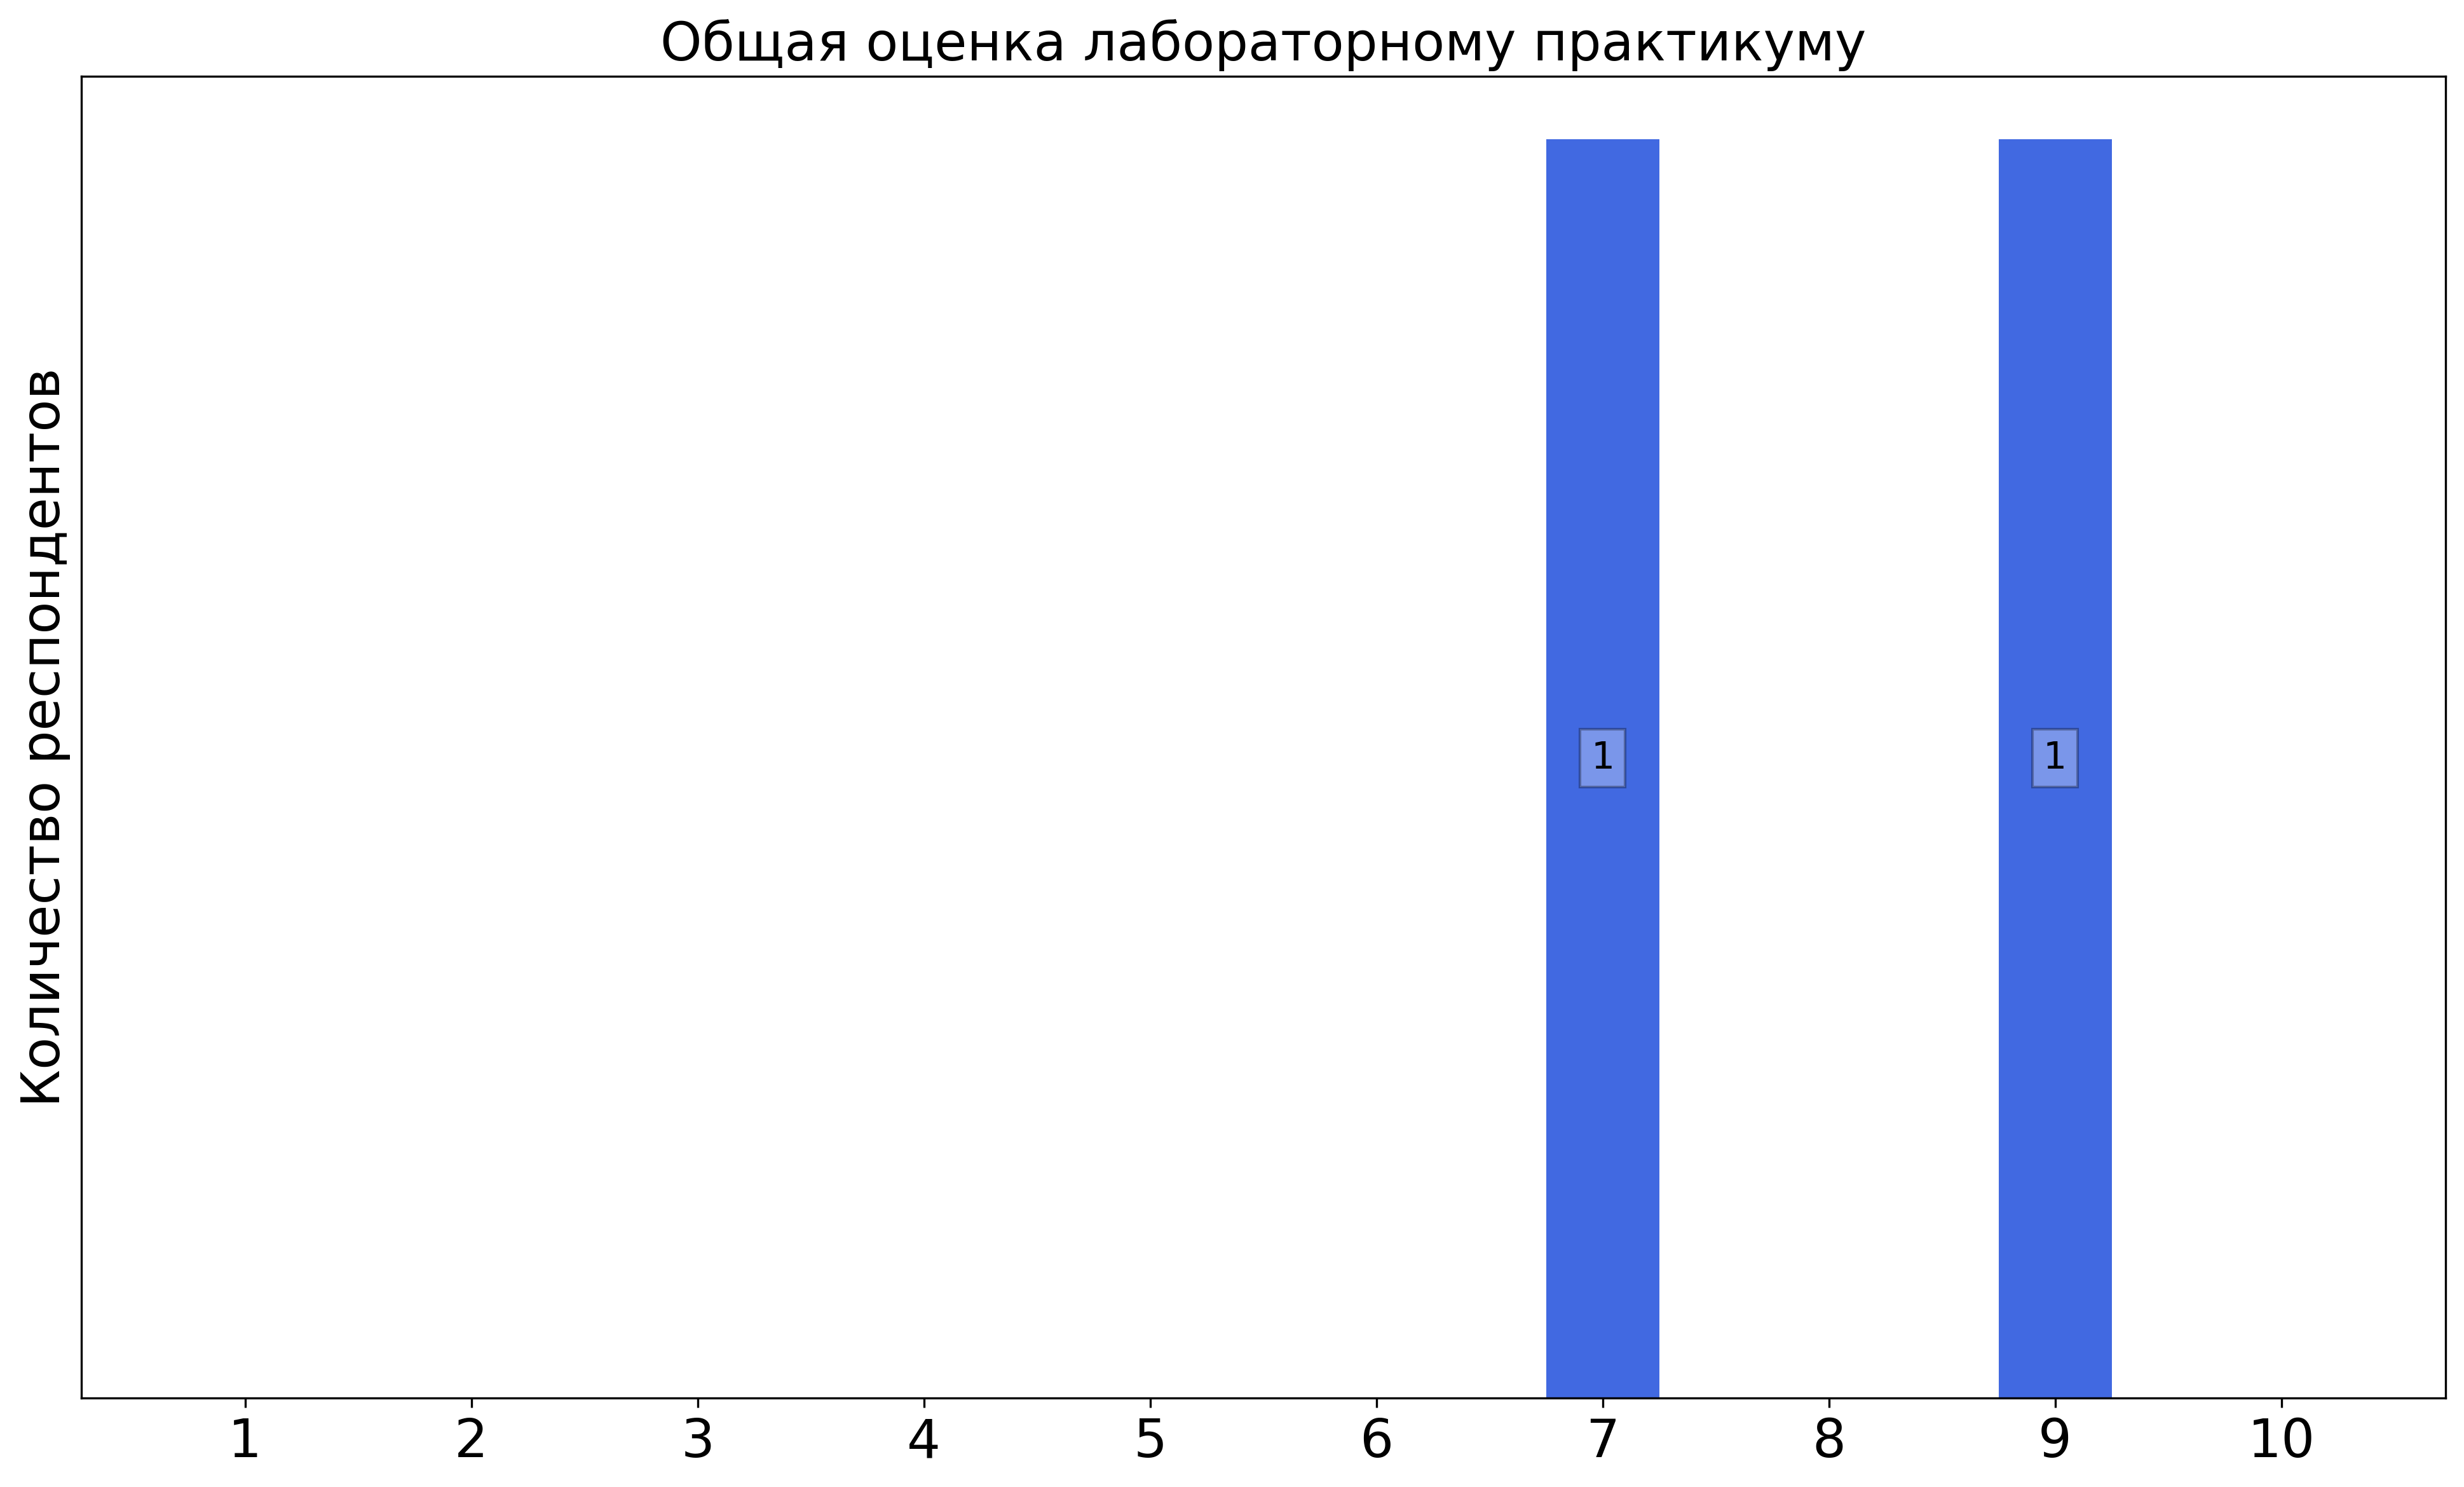
\includegraphics[width=\textwidth]{images/3 course/Радиофизическая лаборатория/labniks-marks-Манукян В.К.-3.png}
			\end{subfigure}	
			\caption{Оценки респондентов о качестве преподавания лабораторных работ}
		\end{figure}

    \subsubsection{Отзыв студентов о лабораторных работах. Преподаватель: Тимофеенко И.А.}
		\begin{figure}[H]
			\centering
			\begin{subfigure}[b]{0.45\textwidth}
				\centering
				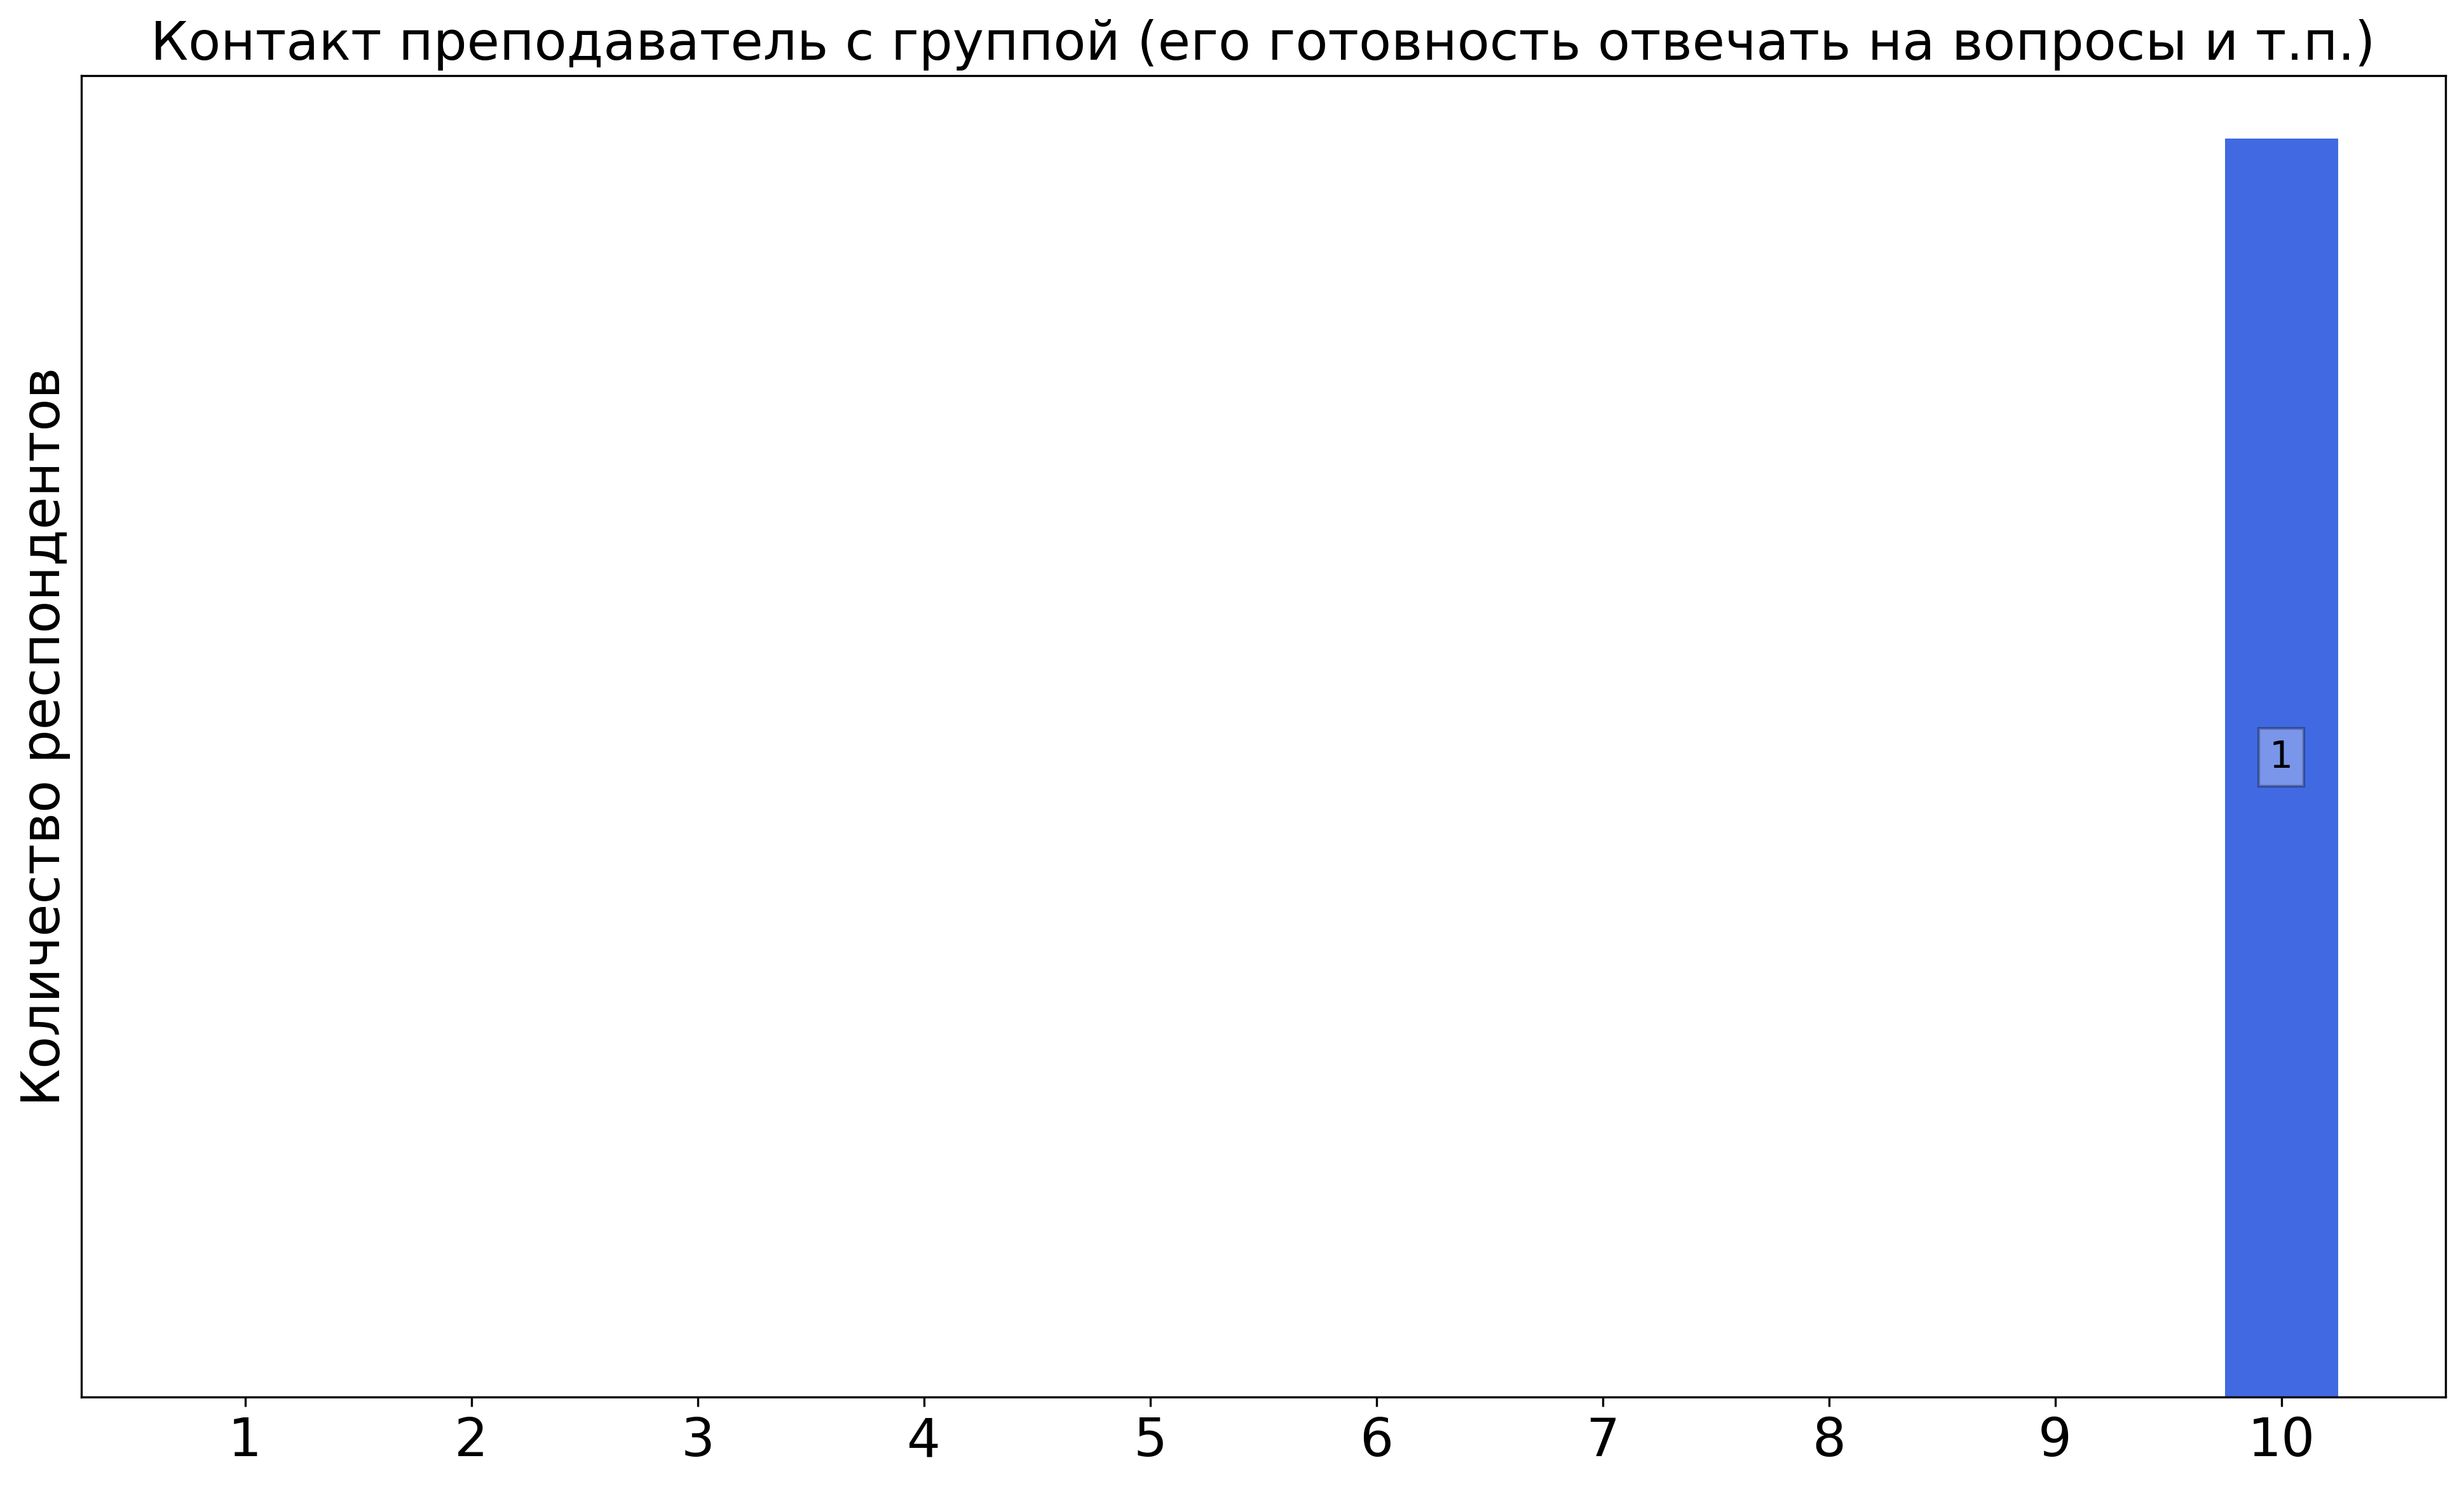
\includegraphics[width=\textwidth]{images/3 course/Радиофизическая лаборатория/labniks-marks-Тимофеенко-0.png}
			\end{subfigure}
			\begin{subfigure}[b]{0.45\textwidth}
				\centering
				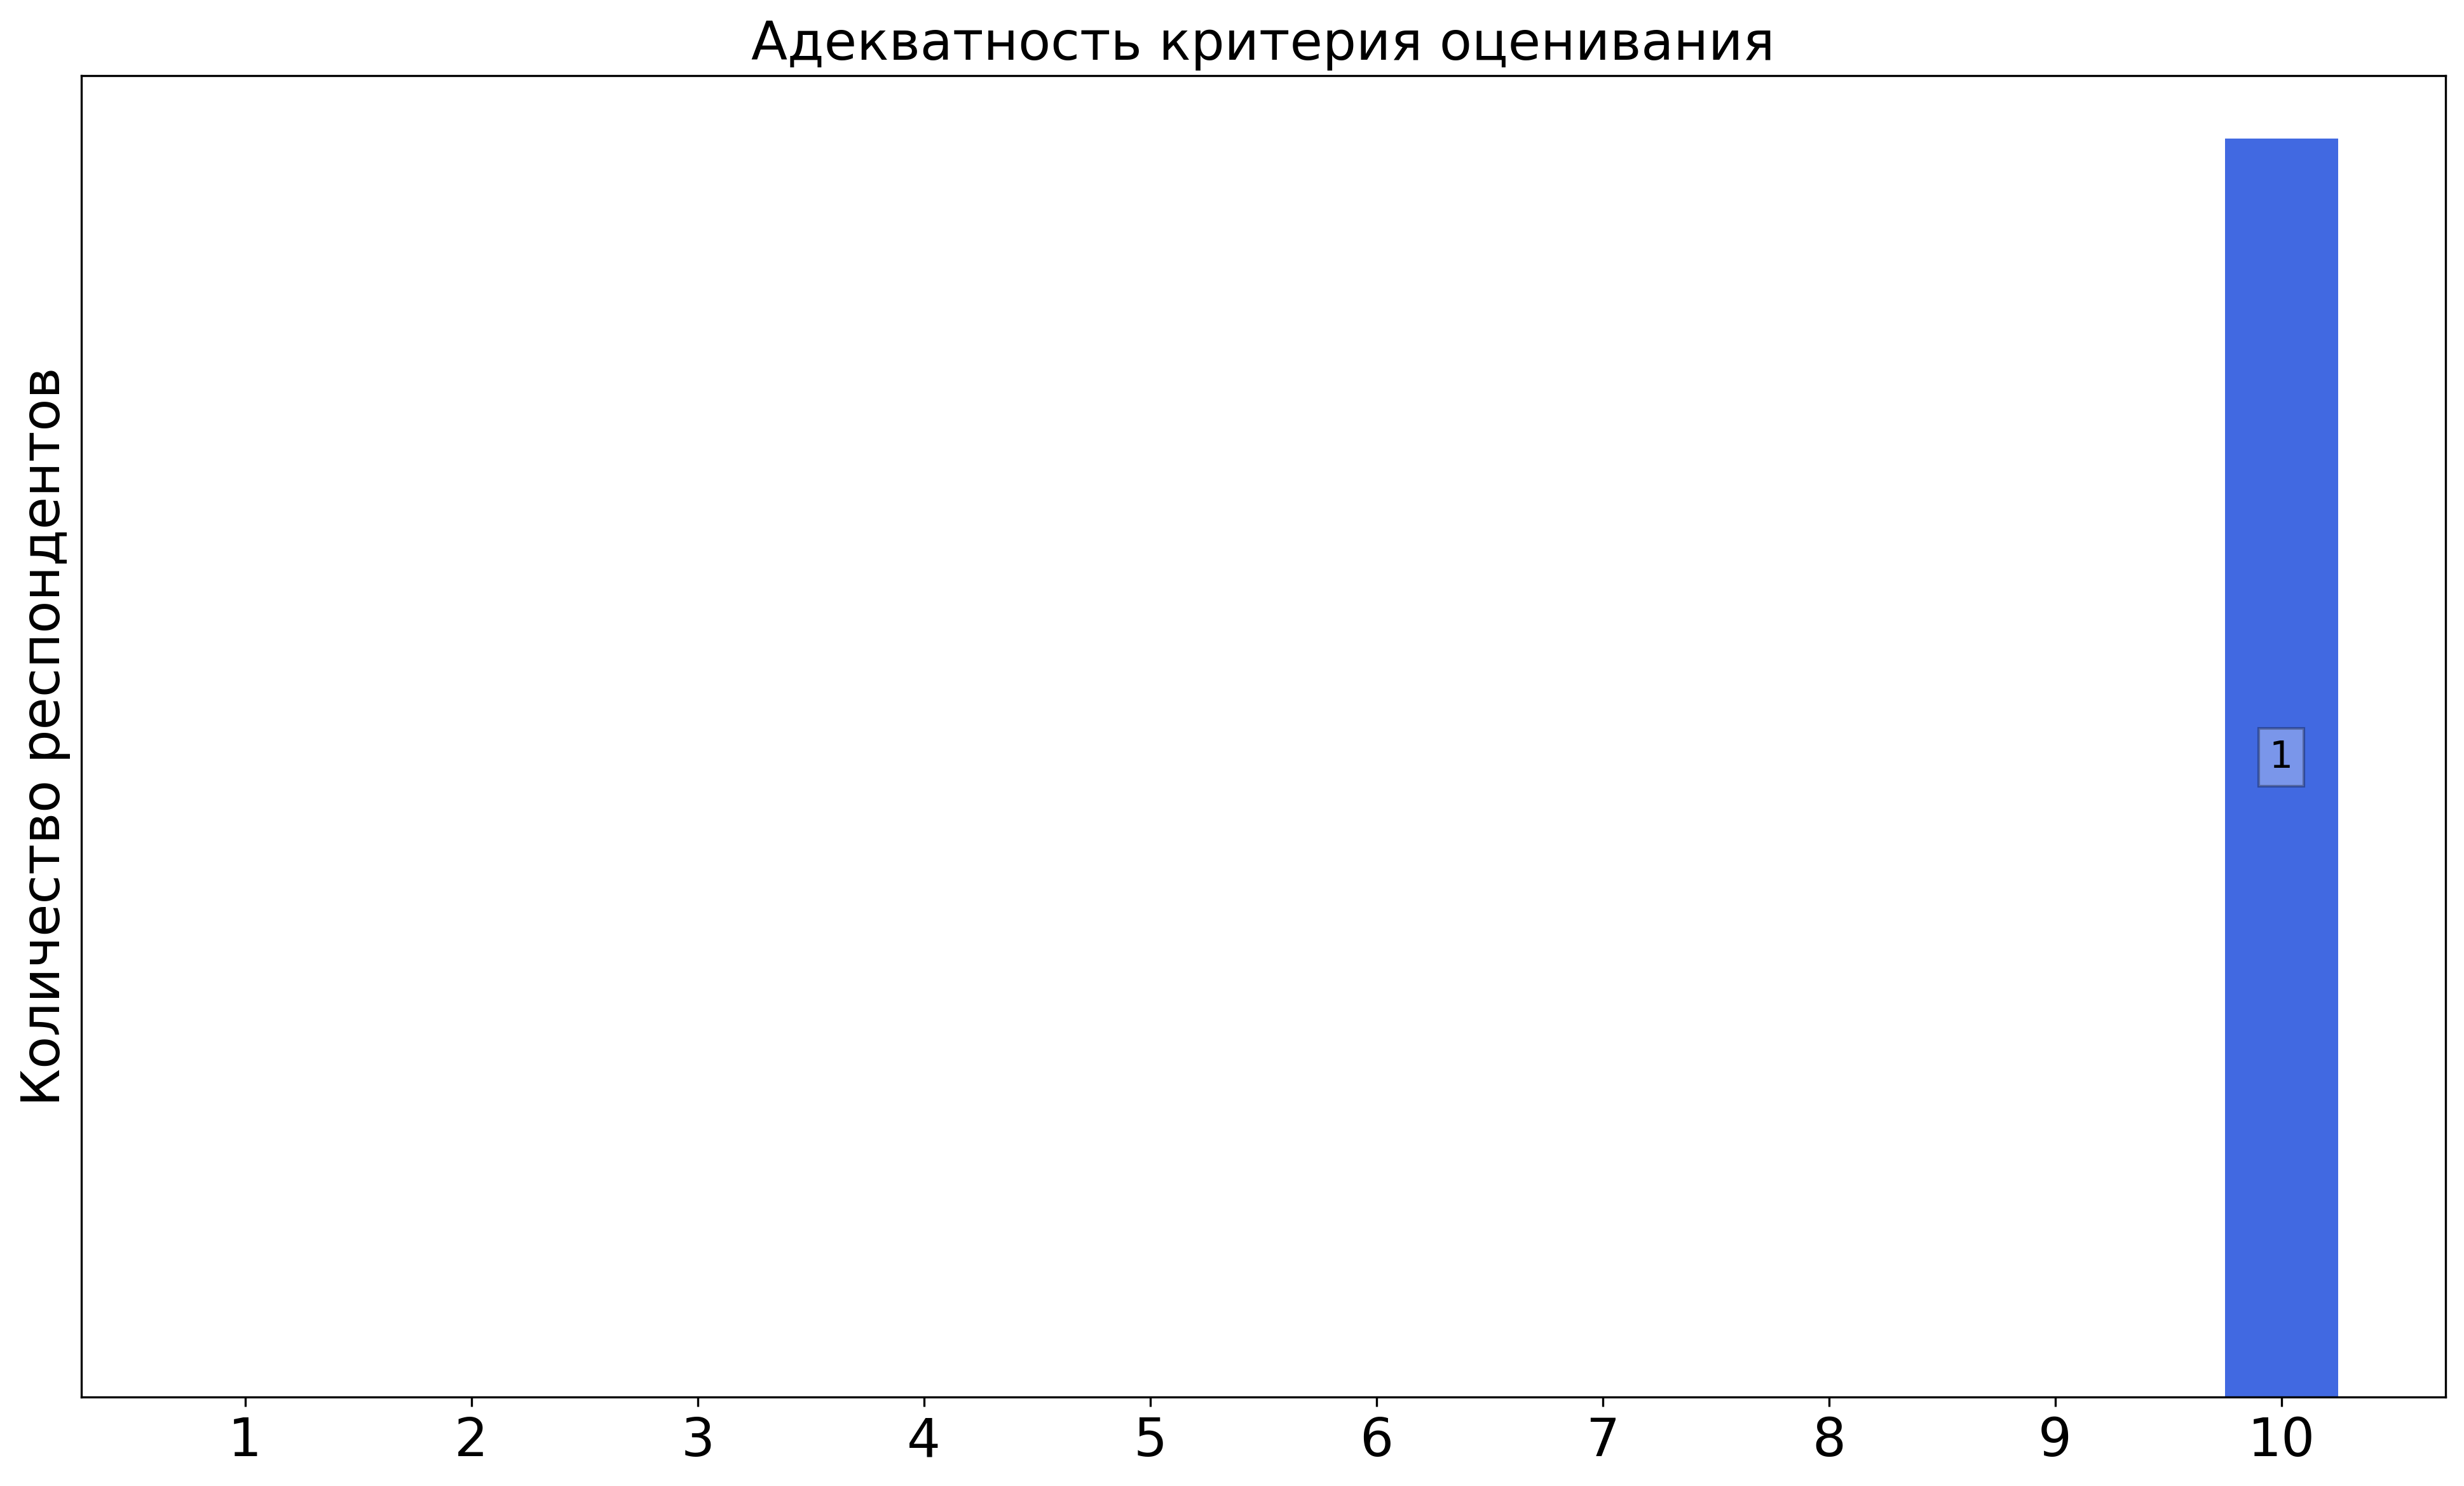
\includegraphics[width=\textwidth]{images/3 course/Радиофизическая лаборатория/labniks-marks-Тимофеенко-1.png}
			\end{subfigure}
			\begin{subfigure}[b]{0.45\textwidth}
				\centering
				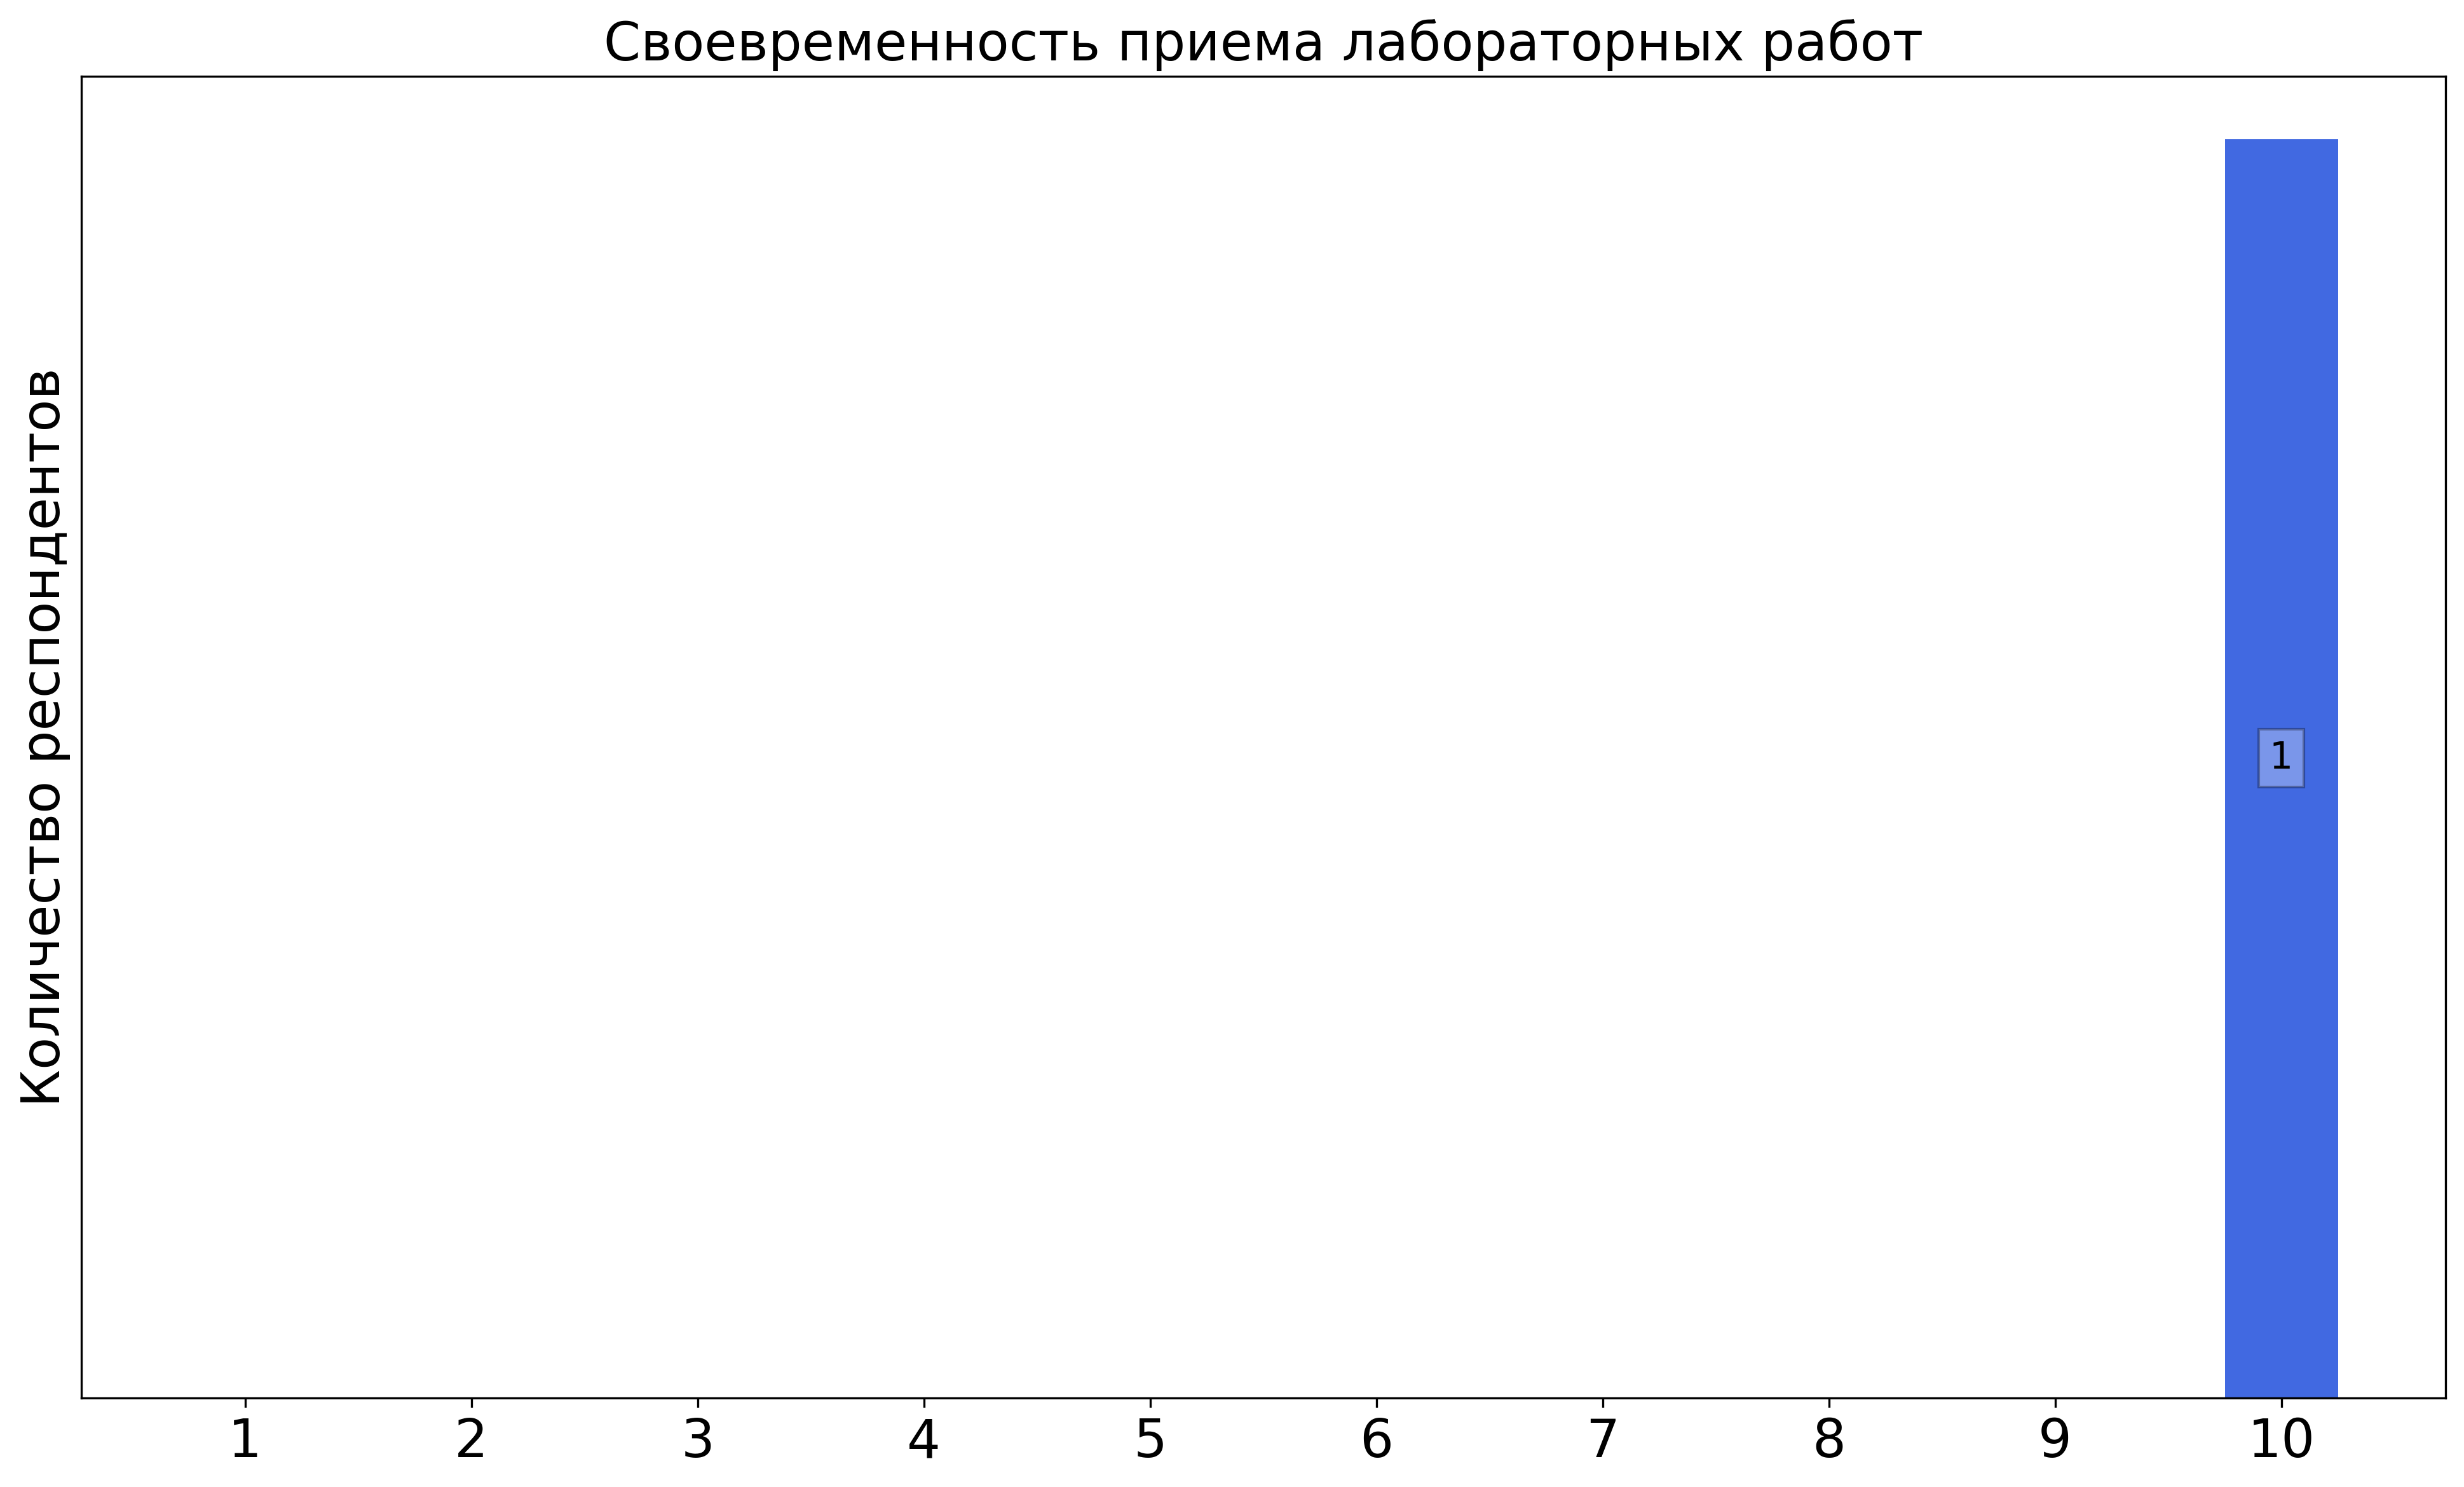
\includegraphics[width=\textwidth]{images/3 course/Радиофизическая лаборатория/labniks-marks-Тимофеенко-2.png}
			\end{subfigure}
			\begin{subfigure}[b]{0.45\textwidth}
				\centering
				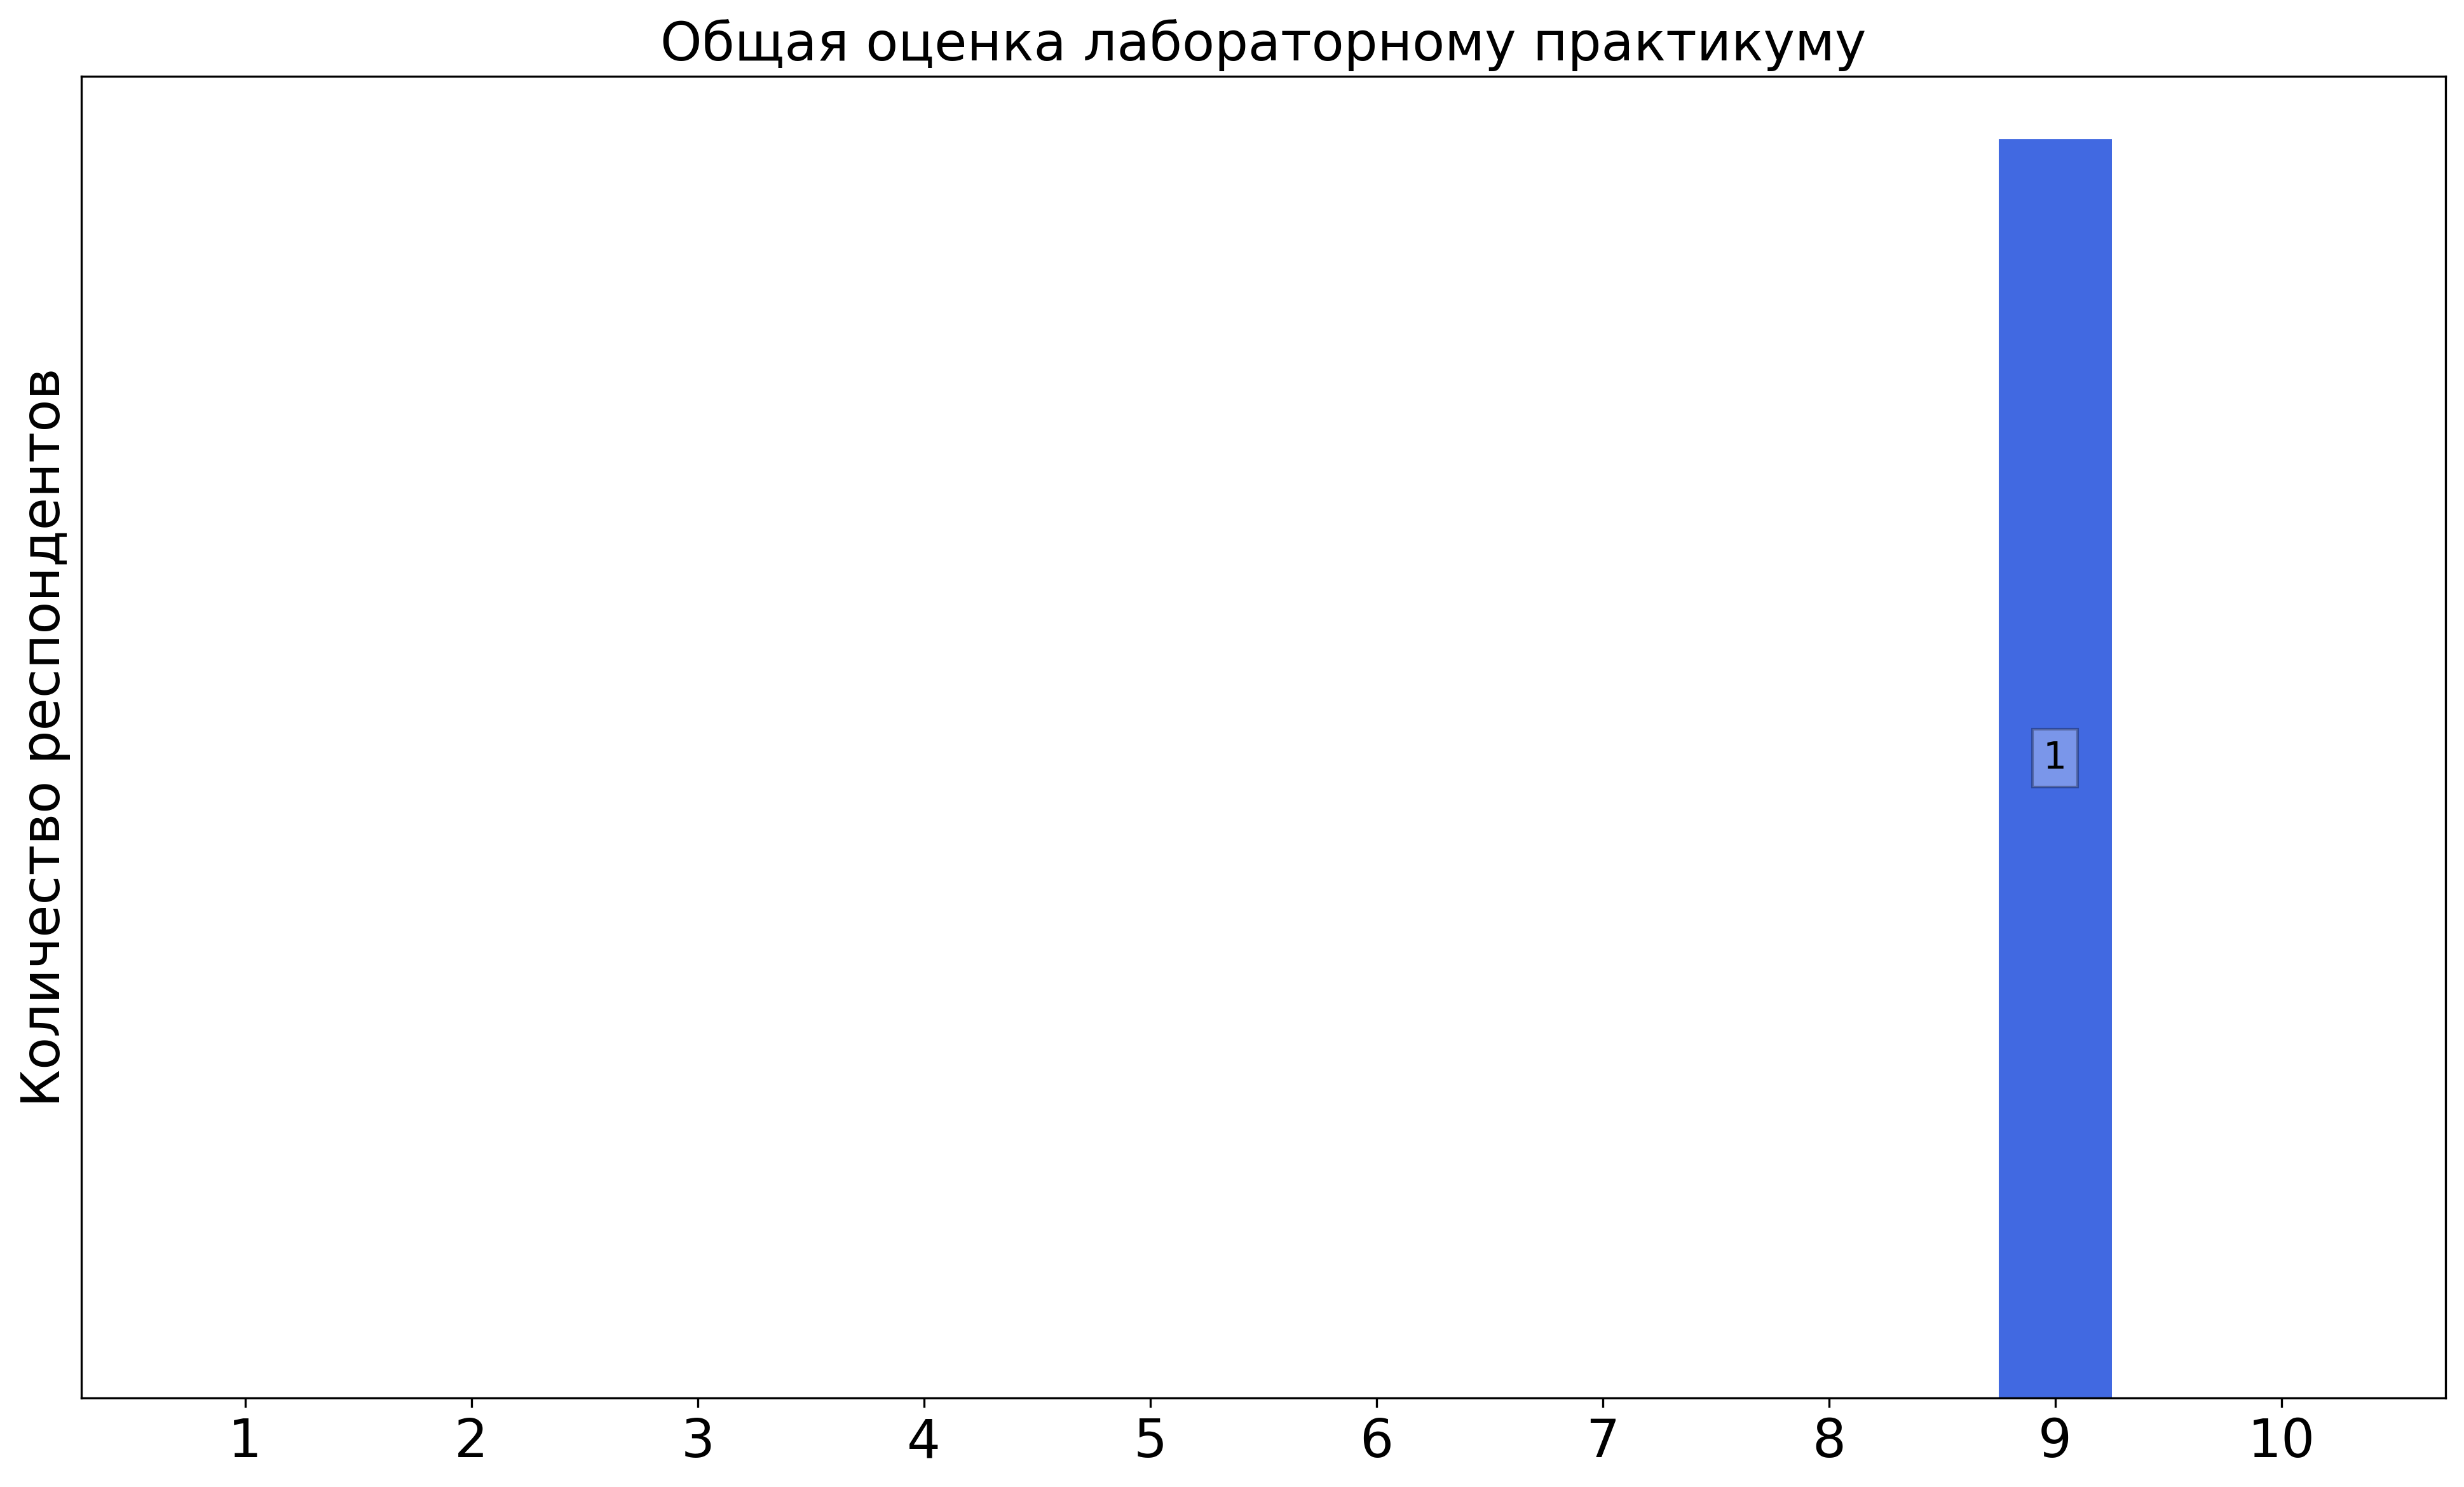
\includegraphics[width=\textwidth]{images/3 course/Радиофизическая лаборатория/labniks-marks-Тимофеенко-3.png}
			\end{subfigure}	
			\caption{Оценки респондентов о качестве преподавания лабораторных работ}
		\end{figure}


    \subsubsection{Отзыв студентов о лабораторных работах. Преподаватель: Тормагов Т.А.}
		\begin{figure}[H]
			\centering
			\begin{subfigure}[b]{0.45\textwidth}
				\centering
				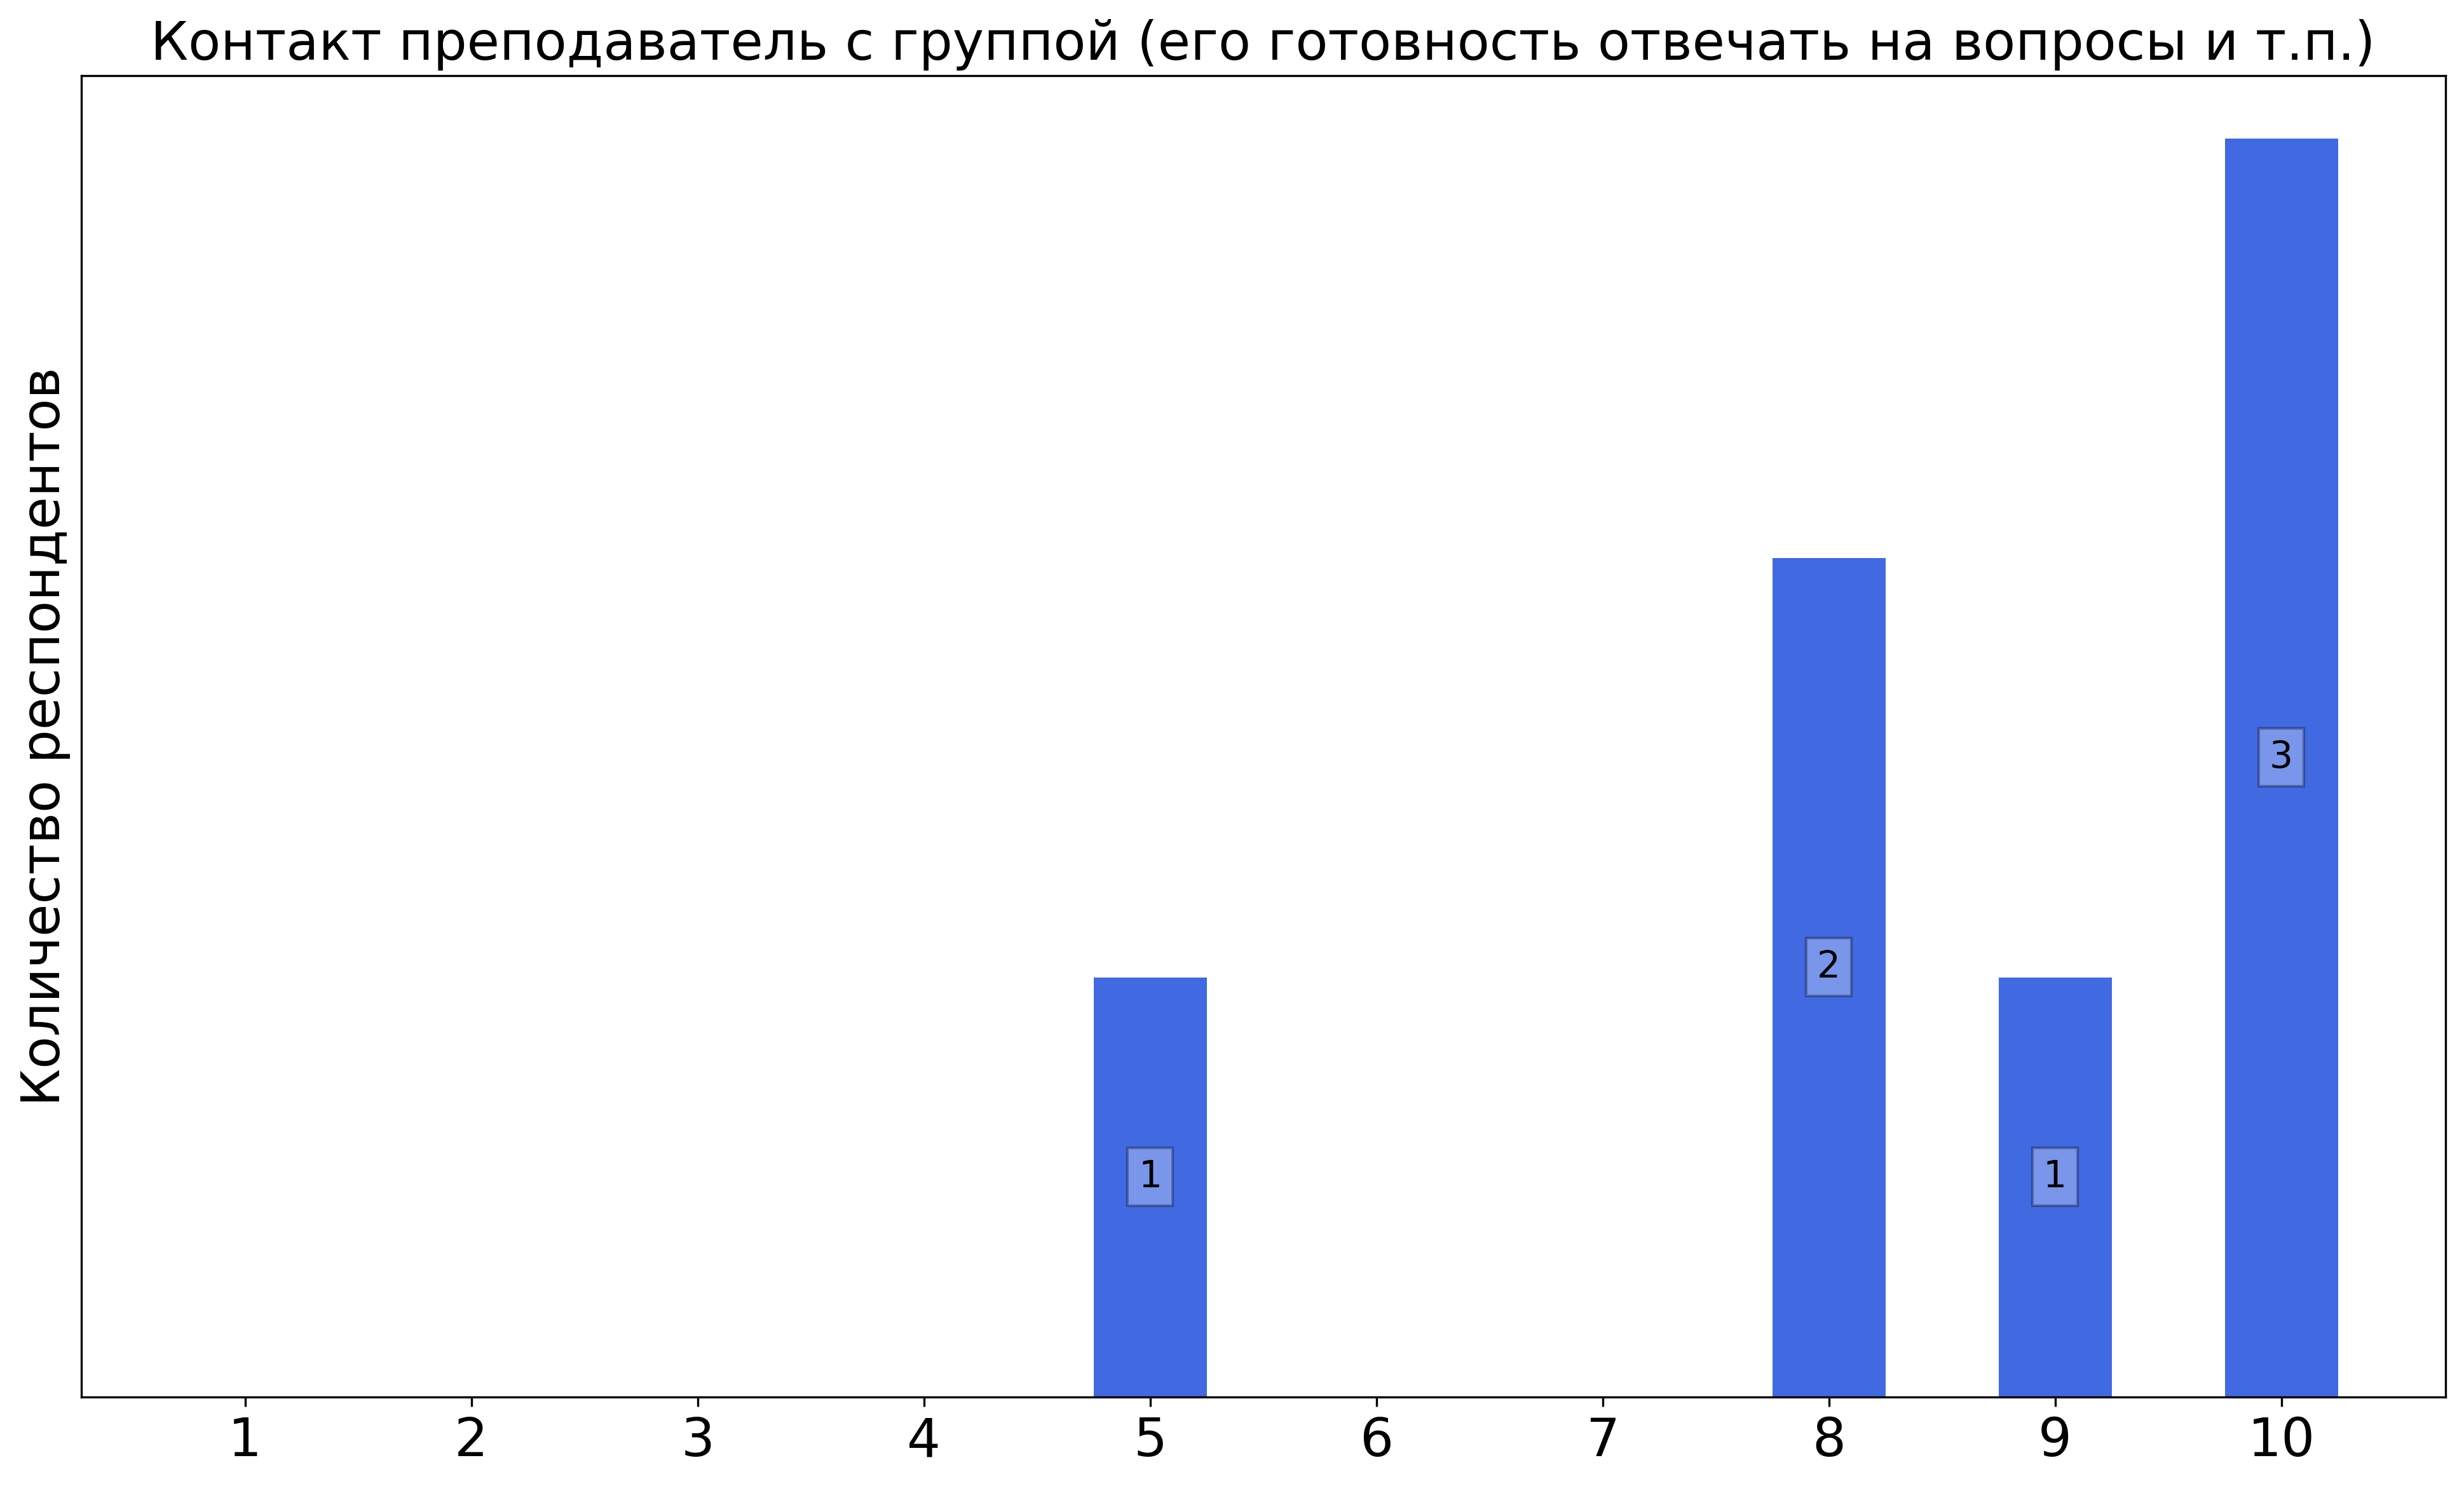
\includegraphics[width=\textwidth]{images/3 course/Радиофизическая лаборатория/labniks-marks-Тормагов Т.А.-0.png}
			\end{subfigure}
			\begin{subfigure}[b]{0.45\textwidth}
				\centering
				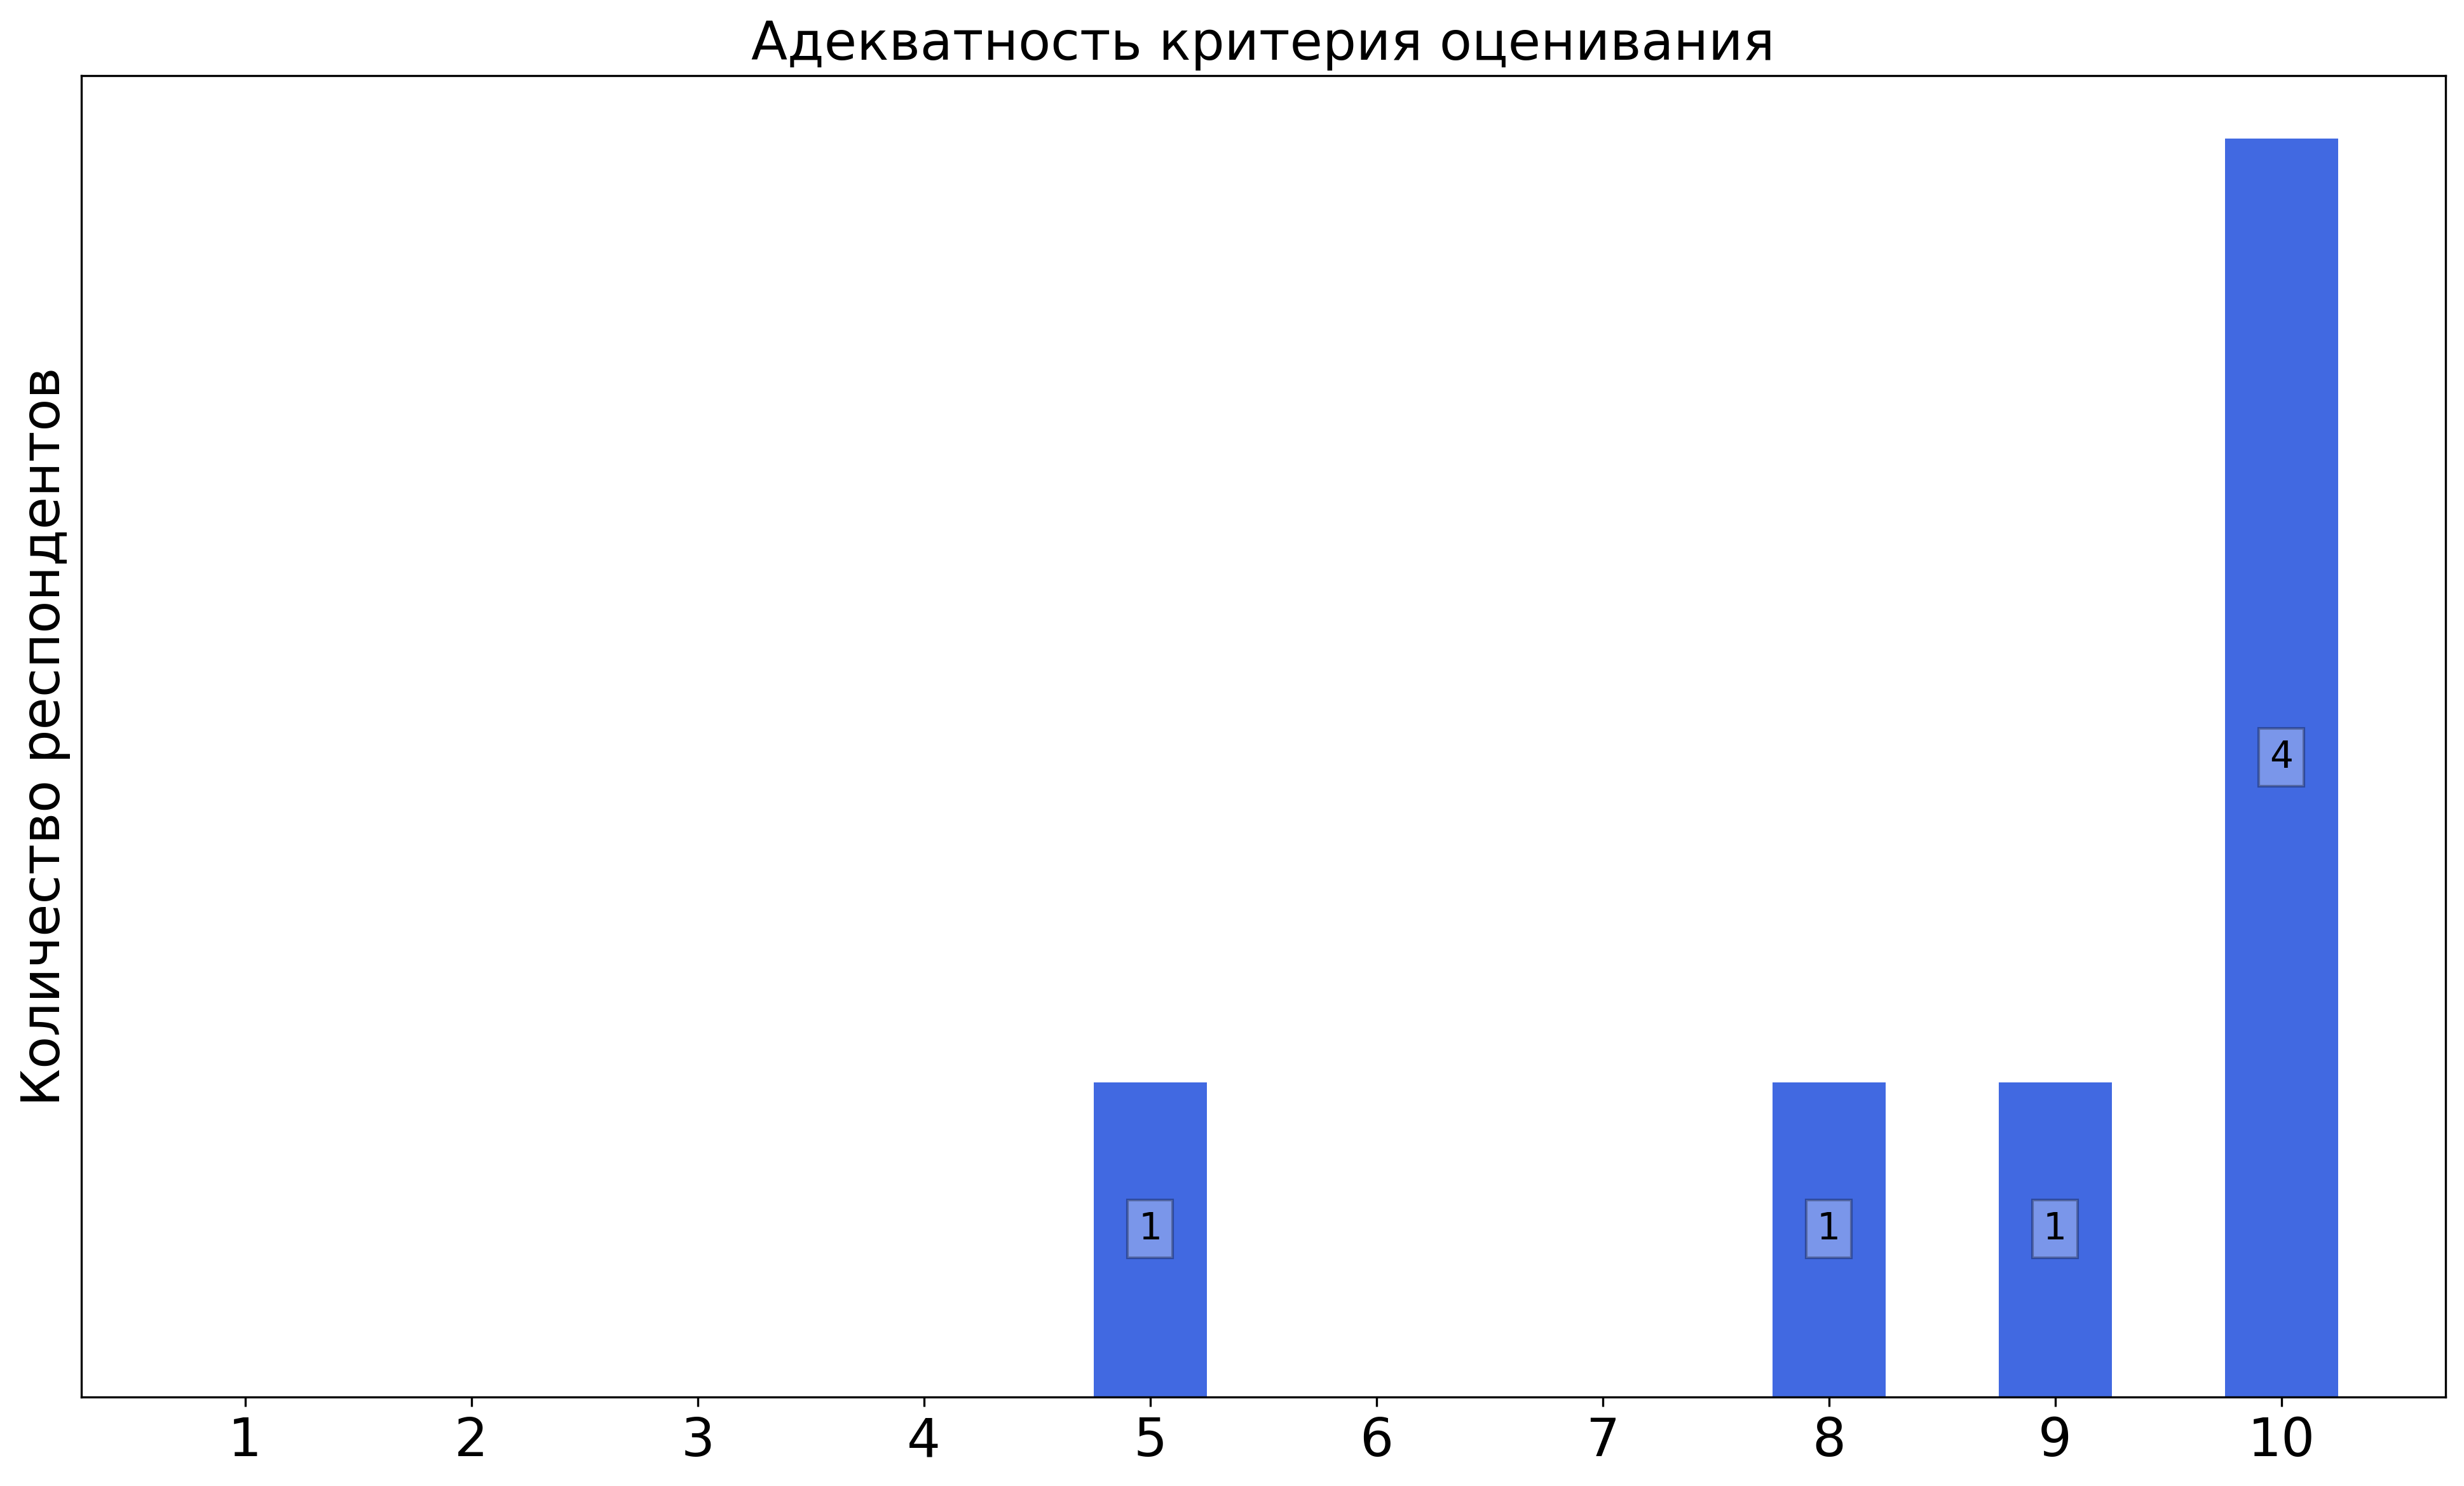
\includegraphics[width=\textwidth]{images/3 course/Радиофизическая лаборатория/labniks-marks-Тормагов Т.А.-1.png}
			\end{subfigure}
			\begin{subfigure}[b]{0.45\textwidth}
				\centering
				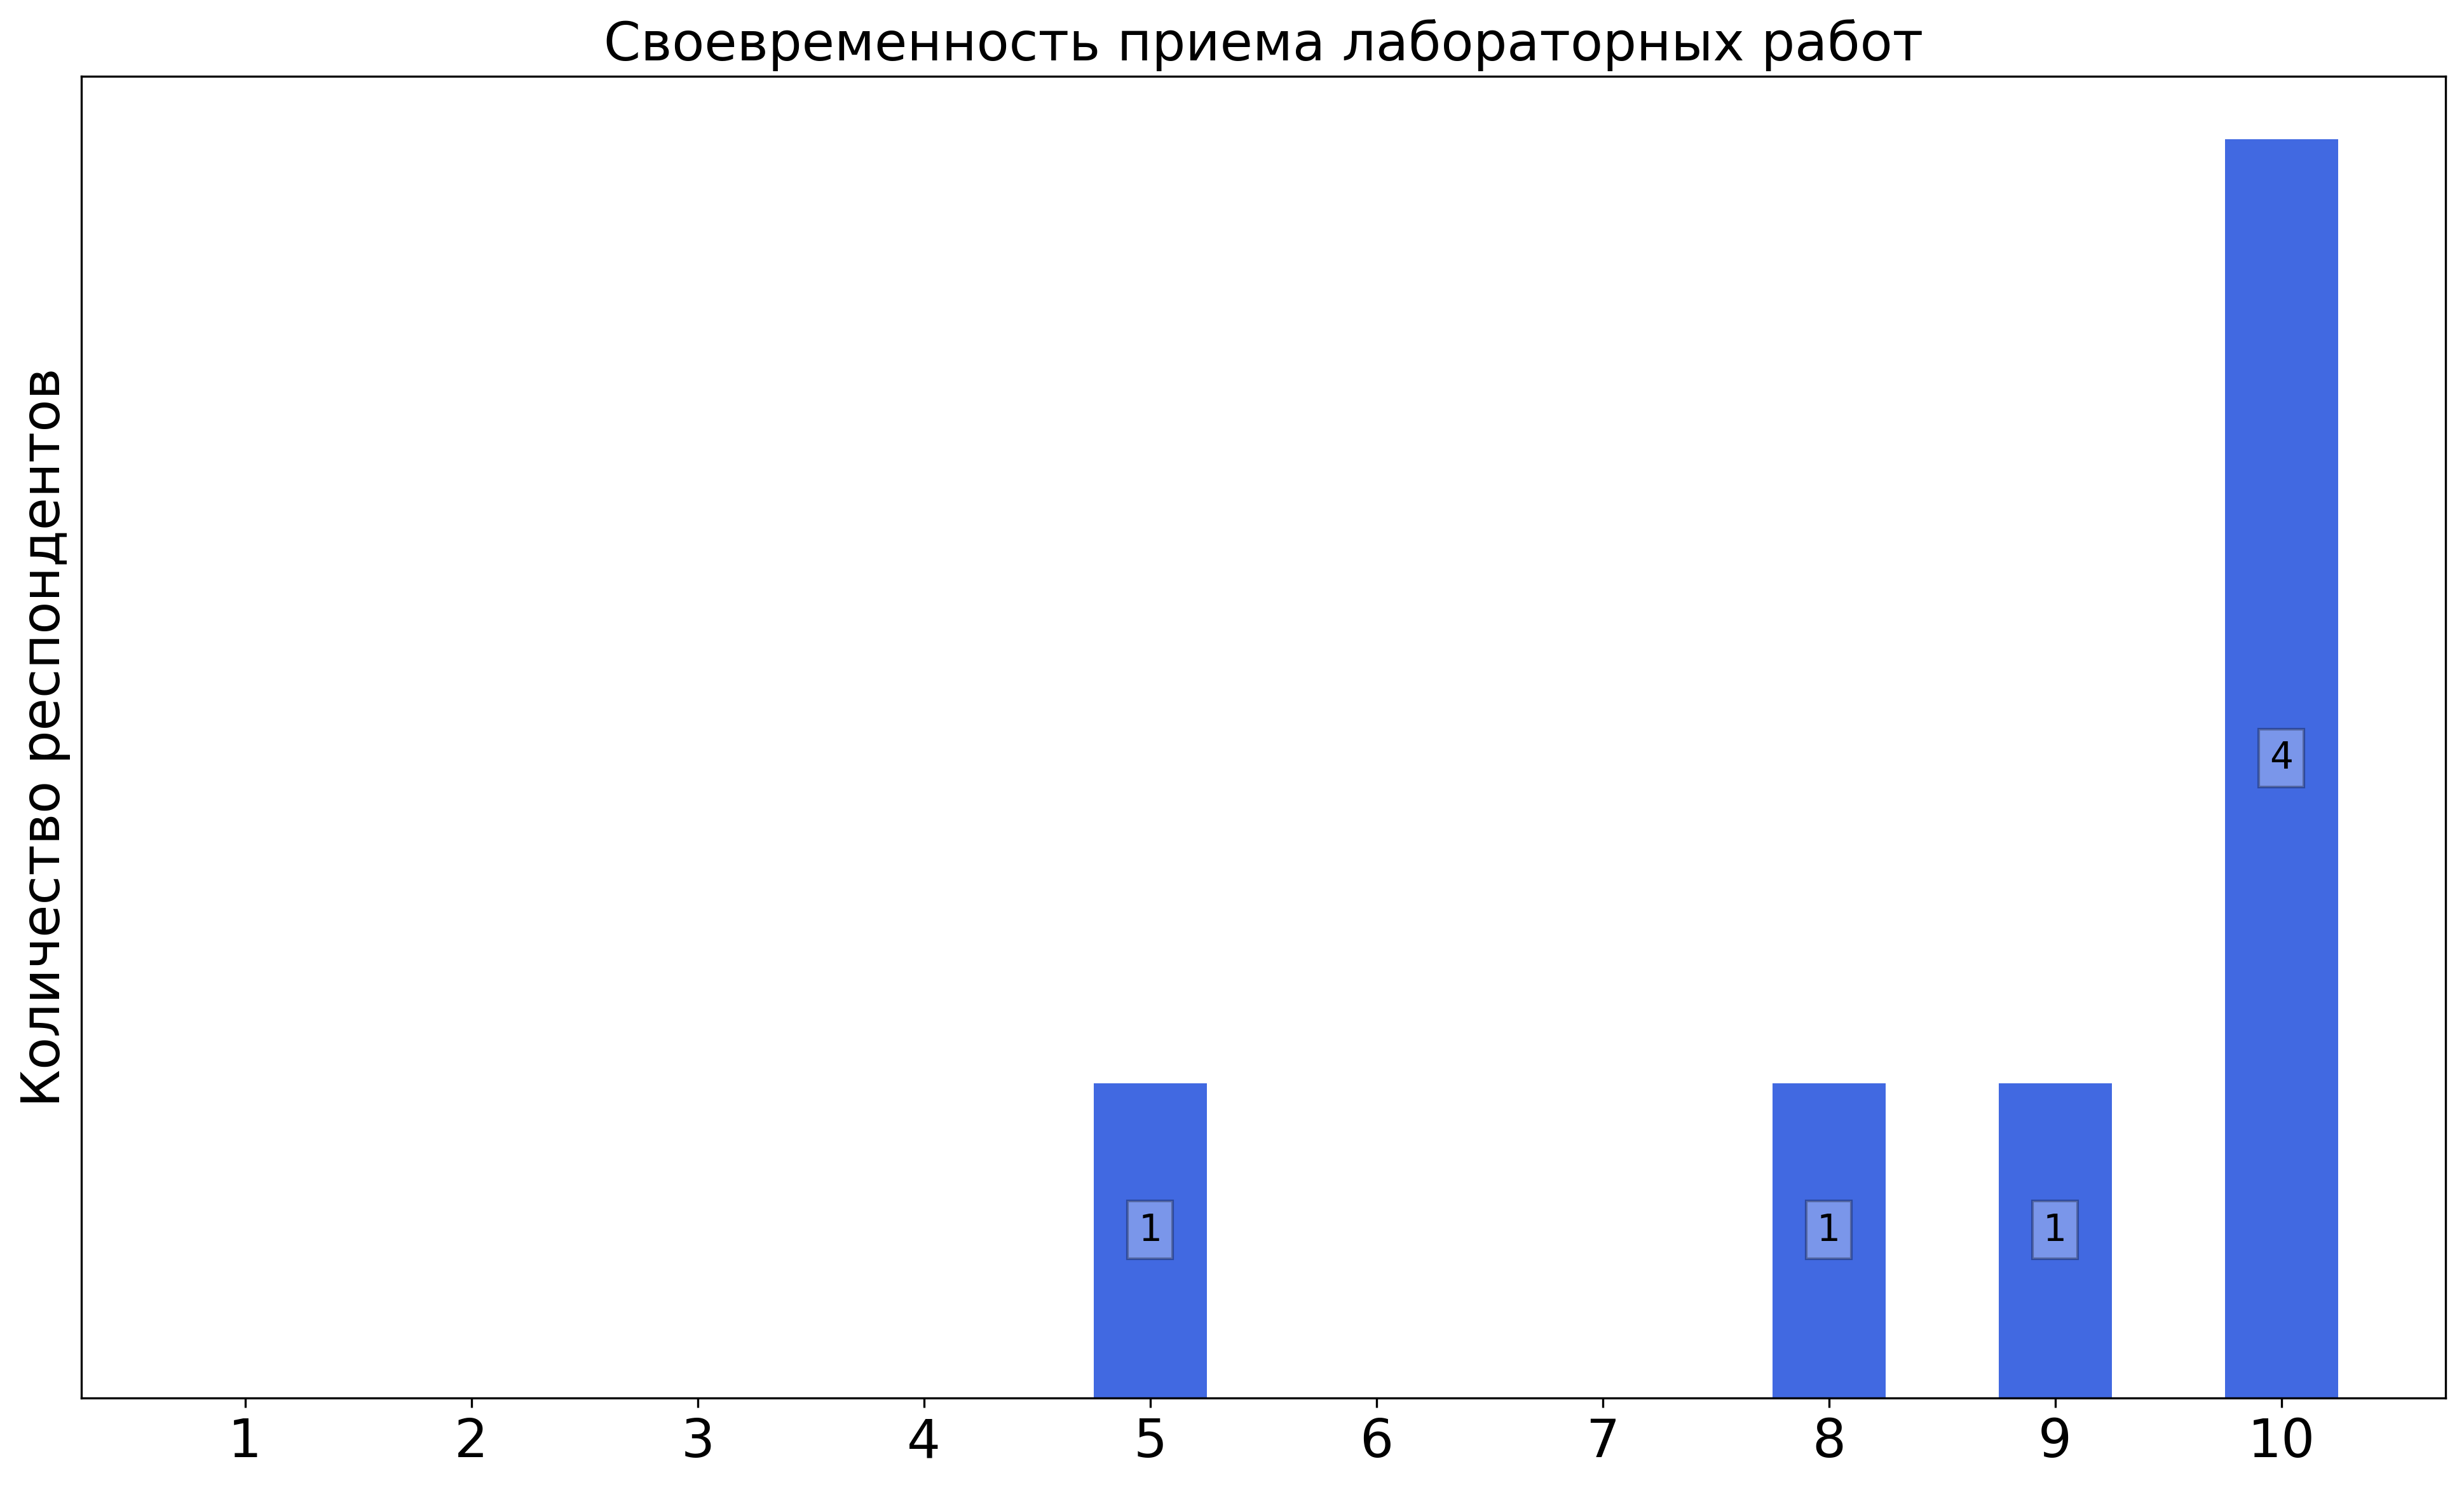
\includegraphics[width=\textwidth]{images/3 course/Радиофизическая лаборатория/labniks-marks-Тормагов Т.А.-2.png}
			\end{subfigure}
			\begin{subfigure}[b]{0.45\textwidth}
				\centering
				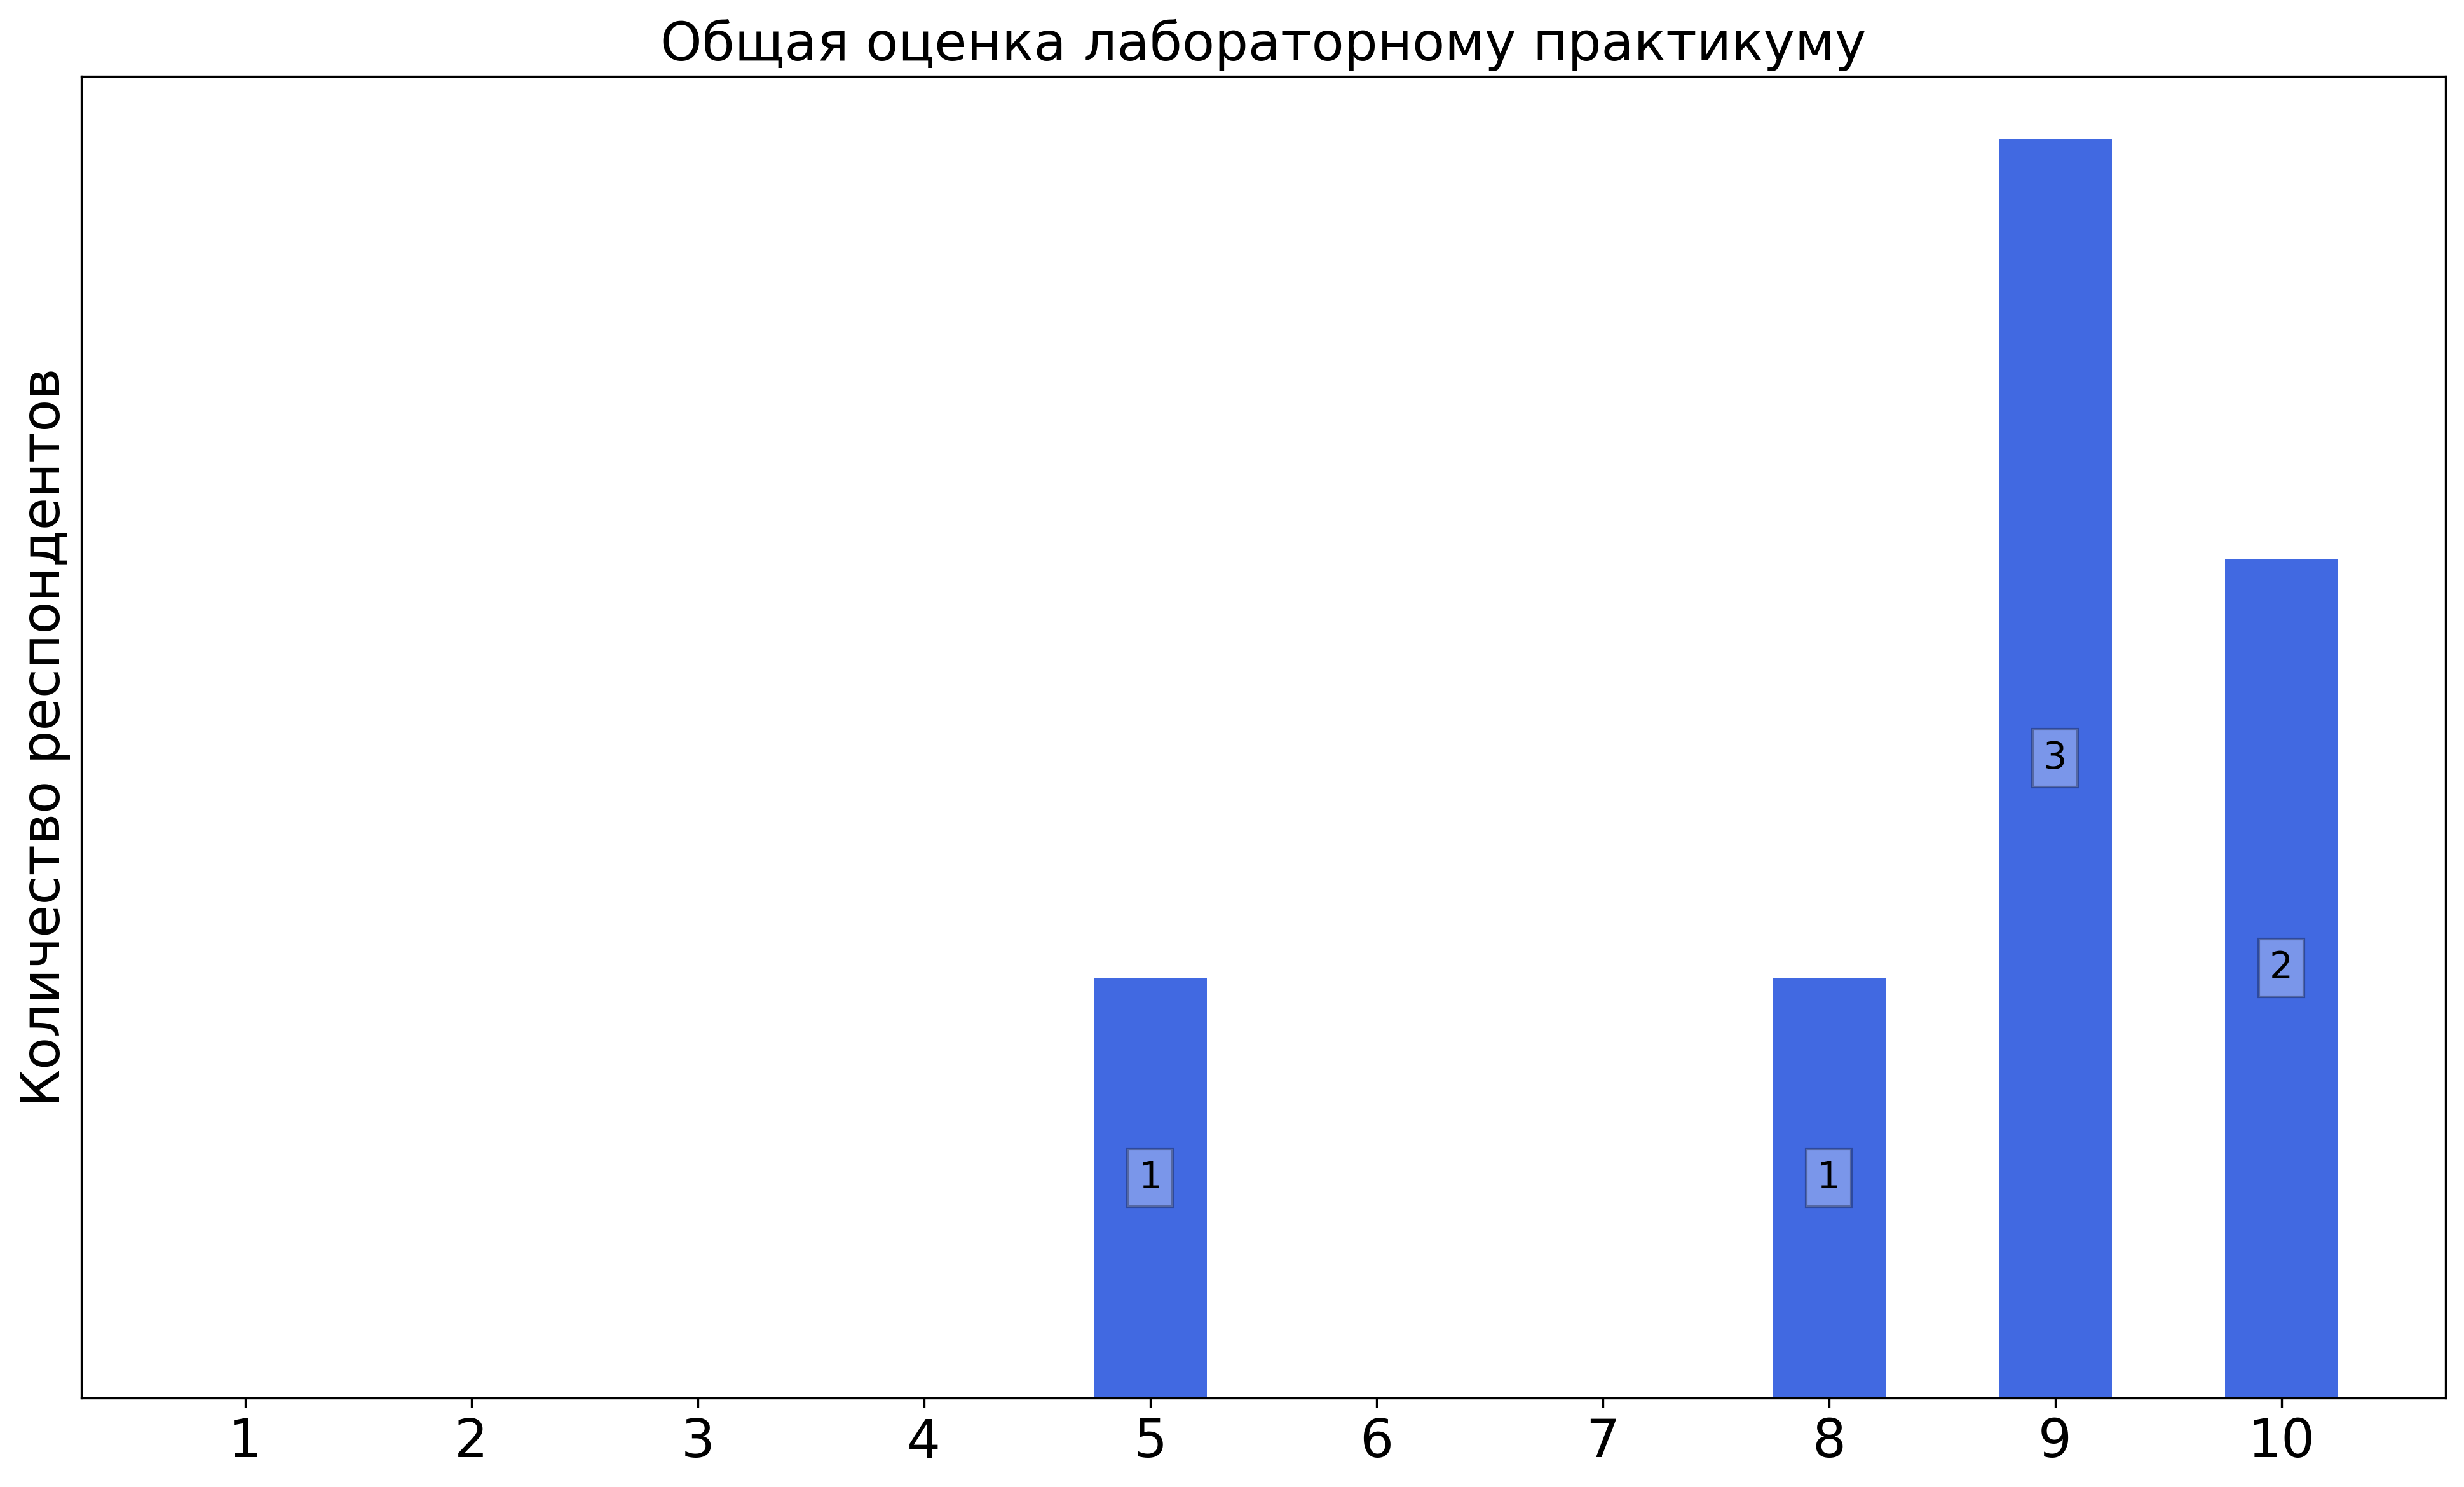
\includegraphics[width=\textwidth]{images/3 course/Радиофизическая лаборатория/labniks-marks-Тормагов Т.А.-3.png}
			\end{subfigure}	
			\caption{Оценки респондентов о качестве преподавания лабораторных работ}
		\end{figure}

		\textbf{Комментарии студентов о преподавателе\protect\footnote{сохранены оригинальные орфография и пунктуация}}
            \begin{commentbox} 
                Тормагов кайфовый, все расшарит 
            \end{commentbox} 

            \begin{commentbox} 
                Единственный минус предмета - его жуткая халявность: кроме 10 никаких оценок не ставят.

                В остальм вопросов нет 
            \end{commentbox} 

            \begin{commentbox} 
                замечательные лабы! Все материалы в удобном формате, классные заготовки к лабам 
            \end{commentbox} 
    
    \subsubsection{Прочие комментарии и предложения по улучшению курса}
		\begin{commentbox}
			Переписать методички, чтобы легче было визуально воспринимать текст
		\end{commentbox}

        \begin{commentbox}
			Очень странная реализация. Как будто он есть ради галочки. Либо убрать его, либо урезать количество информации в одной лабе, либо оценивать жёстче. Тогда смысла будет больше, хотя я бы негодовал
		\end{commentbox}

        \begin{commentbox}
			Убрать его из программы.
		\end{commentbox}

        \begin{commentbox}
			Было бы здорово, если бы курс преподавался только тем студентам, которым он был бы полезен.
		\end{commentbox}
        
        \begin{commentbox}
			Немного непонятный практикум с точки зрения материала, на мой взгляд по-хорошему переносить на более старшие курсы или делать по желанию.
		\end{commentbox}

        \begin{commentbox}
			Начинать читать лекции одновременно с семинарами, т.е. раньше на семестр, чем сейчас. Либо начинать семинары позже на семестр.
		\end{commentbox}

        \begin{commentbox}
			Предмет для галочки, возможно это и не очень хорошо
		\end{commentbox}